\begin{comment}
\chapter{Desarrollo de formulas teóricas}\label{anexoB}
\thispagestyle{fancy}
\pagenumbering{arabic}\renewcommand{\thepage}{B.\arabic{page}}
    En este anexo se presentan el desarrollo detallado de las fórmulas presentadas en el capitulo \ref{CAP4} 
    
    
\section{Método A}
    \subsection{Modelación cinemática de posición}
        \subsubsection{Cinemática directa}
        
        La cinemática directa busca encontrar la posición del centroide del efector en el espacio cartesiano por medio de la configuración del espacio articular de los actuadores del robot delta.
        \begin{equation*}
             \left(  \theta _{1}, \theta _{2}, \theta _{3} \right)   \rightarrow E_{0} \left( x_{0},y_{0},z_{0} \right)            
        \end{equation*}

        \begin{figure}[htb]
            \centering
            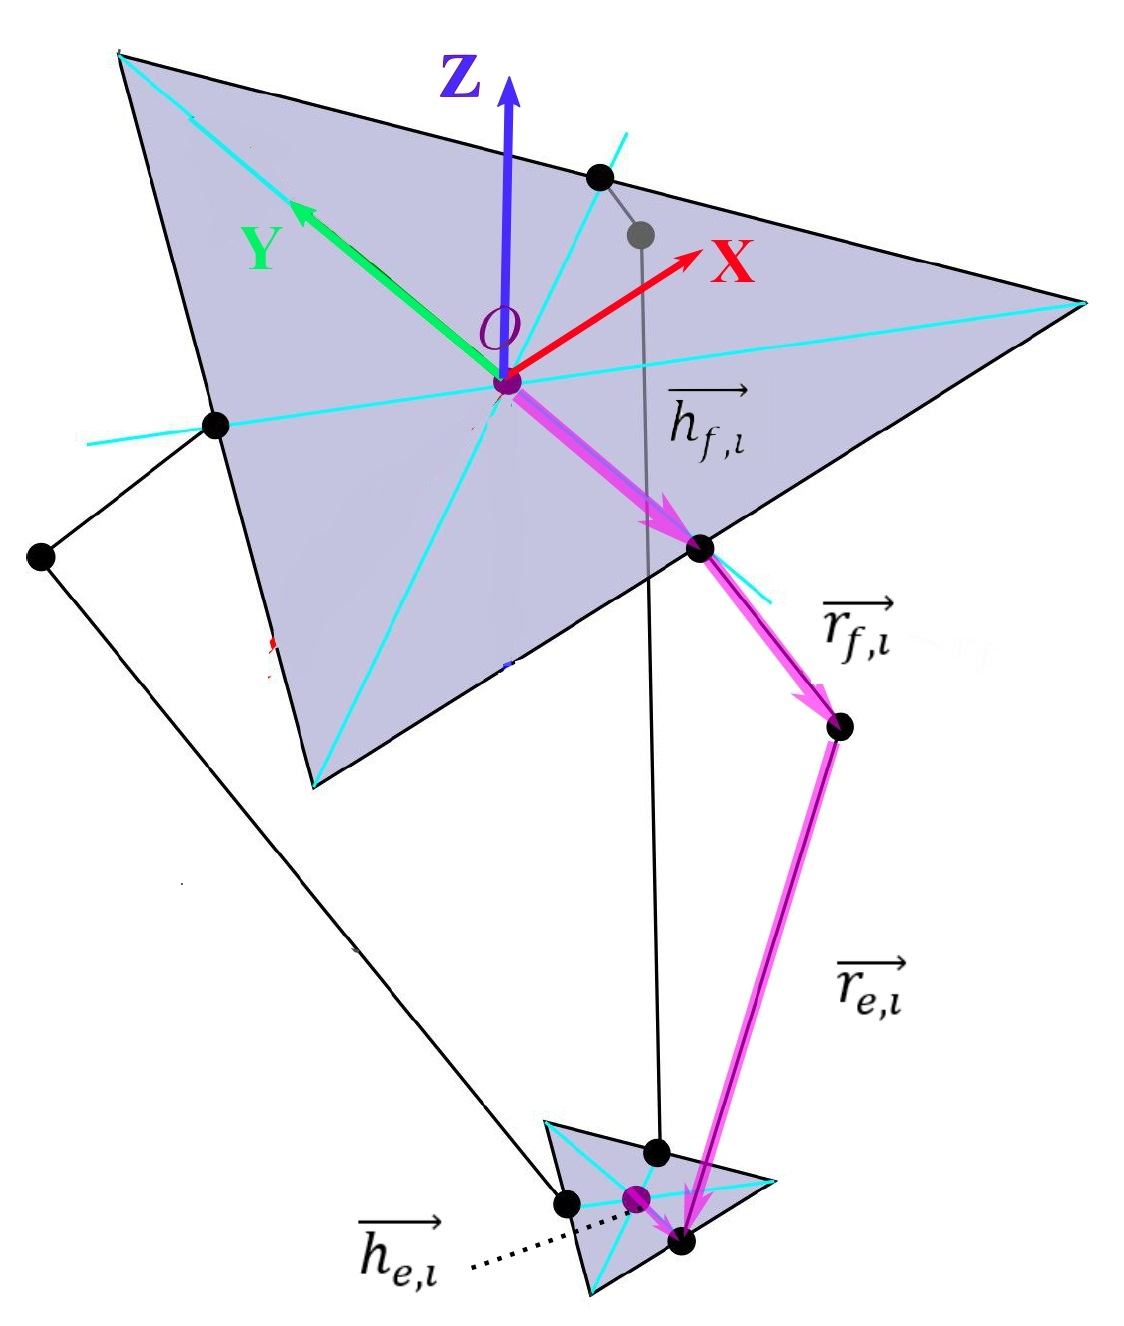
\includegraphics[width=0.45\linewidth]{Main/Chapter4/Images4/DIBUJO10.jpg}
            \caption{Vectorización cinemática directa método A}
            \label{fig:ANEXO_MA_C_POS_1}
        \end{figure}

\newpage


        % Multiples imagenes        
            \begin{figure}
             \centering
                  \subfloat[Representacion grafica desplazamiento del vector que representa el antebrazo hacia el punto $E_0$]{
                   \label{f:gato}
                    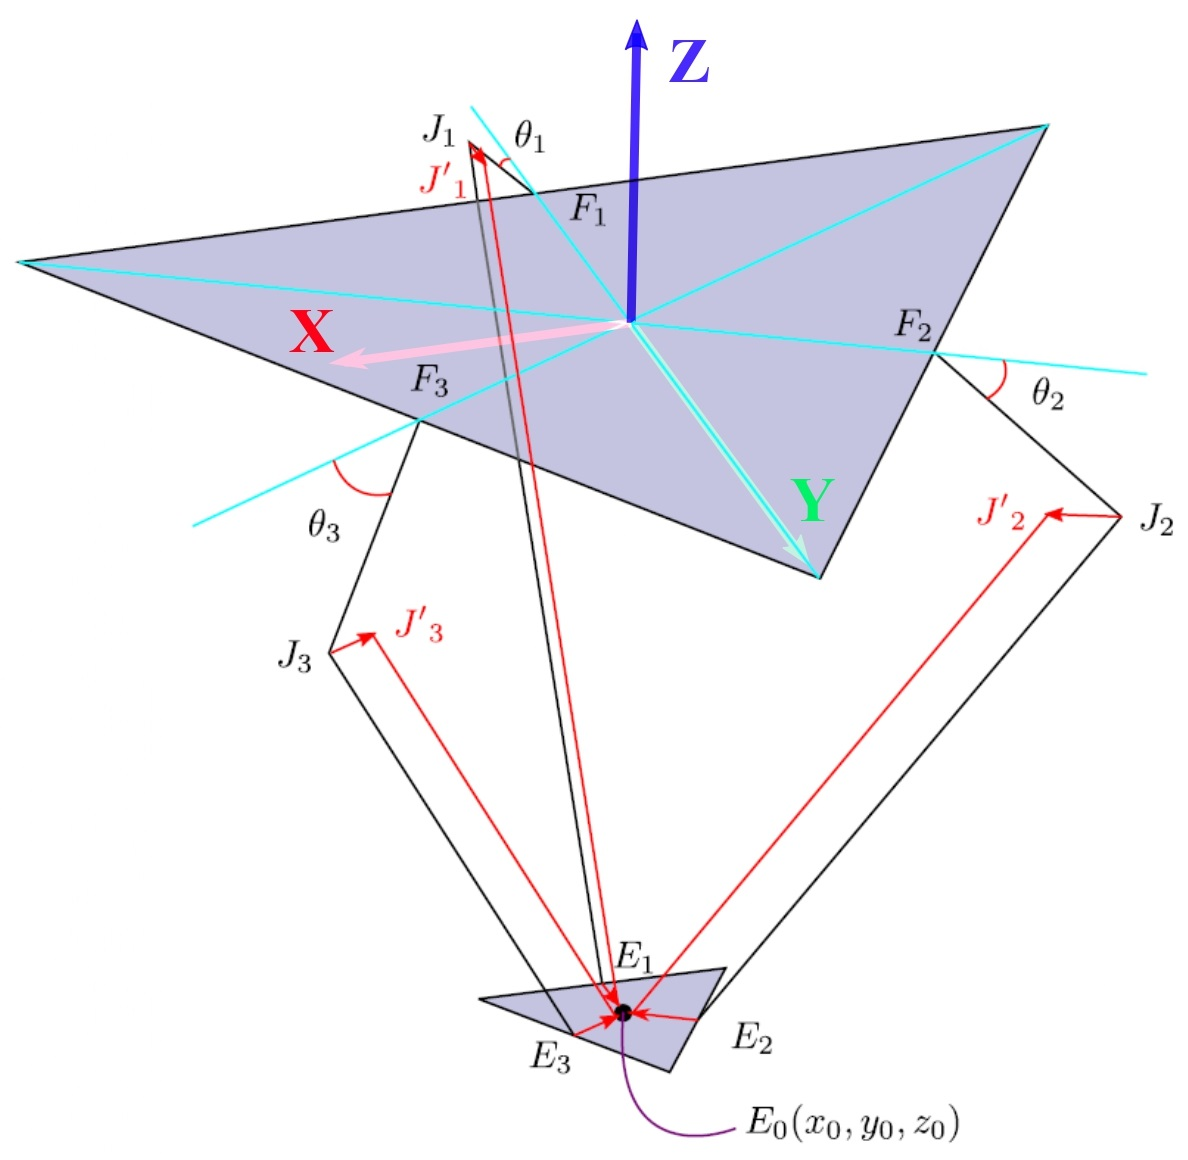
\includegraphics[width=0.5\textwidth]{Main/Chapter4/Images4/DIBUJO7.jpg}}
                  \subfloat[Vista superior base fija]{
                   \label{f:tigre}
                    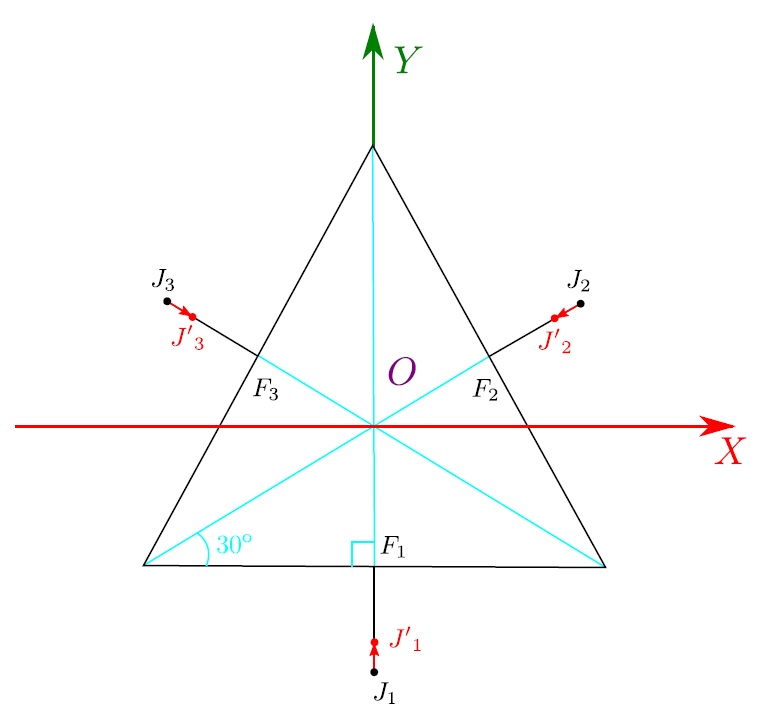
\includegraphics[width=0.5\textwidth]{Main/Chapter4/Images4/DIBUJO8.PNG}}
                 \caption{Desplazamiento de vectores para la solución de la cinemática directa del método A}
                 \label{f:Desplazamiento_J}
            \end{figure}
            
        Las posiciones en el espacio de los vectores $\overrightarrow{r_{f,i}}$  , que representa los brazos del robot delta, ya están definidos en magnitud y sentido debido a que se conoce los ángulos de los actuadores    $\left(  \theta _{1}, \theta _{2}, \theta _{3} \right)$   y la longitud de los brazos.
        
        Sobre el vector  $\overrightarrow{r_{e,i}}$  ,que representa los antebrazos, solo se conoce el punto inicial  $J_{i}$  que coincide con el extremo del vector   $\overrightarrow{r_{f,i}}$  . En consecuencia, la orientación para cada vector $\overrightarrow{r_{e,i}}$  , está restringido por una esfera con centro en la junta esférica  $J_{i}$ , que conecta el brazo con el antebrazo, con radio equivalente al largo del antebrazo  $r_{e}$ .
        
        Finalmente, para obtener las coordenadas del centroide del efector final   $E_{0} \left( x_{0},y_{0},z_{0} \right)$   , se realiza una traslación de las esferas mencionadas anteriormente. Esta traslación depende de la dirección y longitud del vector   $\overrightarrow{h_{e,i}}$   para cada cadena x respectivamente. Se genera 3 nuevas esferas, con centros en   $J'_{i}$   y de radio equivalente al largo del antebrazo   $r_{e}$  . Estas esferas trasladadas se intersectan en un punto en común, el centroide del efector   $E_{0} \left( x_{0},y_{0},z_{0} \right)$  . Por lo tanto, se calculan las coordenadas del punto  $E_{0} \left( x_{0},y_{0},z_{0} \right)$    realizando un sistema de ecuaciones no lineal con 3 restricciones impuestas por las 3 esferas.
        
        El primer paso para calcular el centroide del efector final  $E_{0}$  es encontrar una manera de representar las posiciones de las juntas  $J_{i}$  (brazo-antebrazo) con los parámetros conocidos. Por medio de geometría básica se pueden determinar otros parámetros para representar el punto   $J_{i}$, como se puede visualizar en la figura \ref{f:Desplazamiento_J}.
        
        El efector tiene forma geométrica de un triángulo equilátero y se tienen las dimensiones de los lados (e), por ende, se puede determinar la magnitud del desplazamiento de las esferas $J_{i}J'_{i}$ de la siguiente manera:
        
        \begin{equation*}
            J_{1}J'_{1}=J_{2}J'_{2}=J_{3}J'_{3}=\frac{e}{2}tan30=\frac{e}{2\sqrt{3}}
        \end{equation*}
    
\newpage
    
            \begin{figure}[htb]
            \centering
            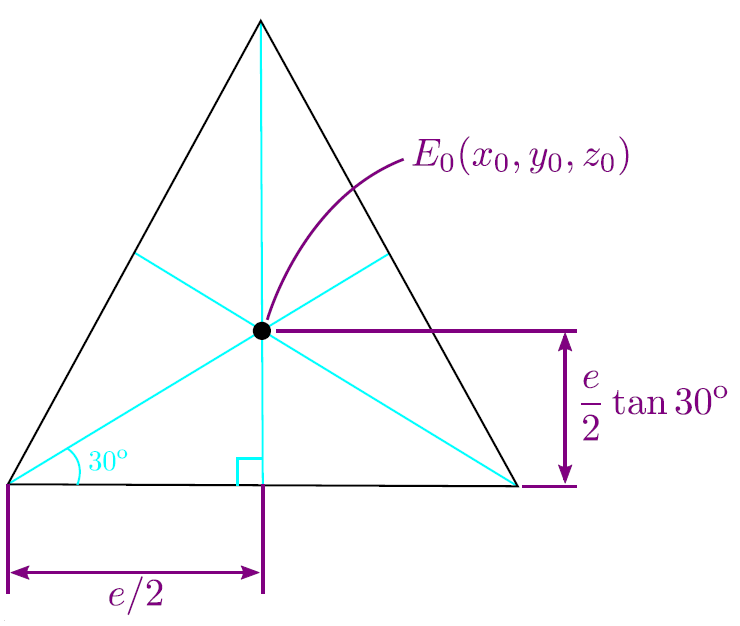
\includegraphics[width=0.5\linewidth]{Main/Chapter4/Images4/DIBUJO9.PNG}
            \caption{Vista superior del efector fijal}
            \label{fig:ANEXO_MA_C_POS_2}
        \end{figure}

        Similar a como se calcula el desplazamiento de las esferas $J_{i}~J'_{i}$, se determina la magnitud de la distancia entre el centroide de la base fija y la posición de los actuadores $OF_{i}$ :
        
        \begin{equation*}
            OF_{1}=OF_{2}=OF_{3}=\frac{f}{2}tan30=\frac{f}{2\sqrt{3}}
        \end{equation*}
        
        La distancia perpendicular entre el plano que contiene la base fija y el punto donde se encuentra las juntas esféricas $J_{i}$  que unen los brazos con sus antebrazos, está en función de cada ángulo de los actuadores $i=1,2,3$, dada por la siguiente ecuación:
        
        \begin{equation*}
            F_iJ_i=r_fcos(\theta_i) , \forall i=1,2,3
        \end{equation*}
        
        Por lo tanto, los centros de las esferas de radio $r_e$ que se intersectan en el centroide  $E_{0} \left( x_{0},y_{0},z_{0} \right)$ del efector son:
        
                \begin{center}
        \renewcommand{\arraystretch}{2.5}
        
            \begin{table}[H]
            \centering
            \begin{tabular}{c c } 
                 \hline
                 \textbf {Centros esferas}\\ [0.1ex] 
                 \hline\hline
                         $\left(x_1,y_1,z_1\right)$ =
                         ${J^'}_1\left(0,\left[-\frac{f-e}{2\sqrt{3}}-r_f{\mathrm{cos} \left({\theta }_1\right)\ }\right],-r_f{\mathrm{sin} \left({\theta }_1\right)\ }\right)$\\ 
                \hline
                          $\left(x_2,y_2,z_2\right)$ = ${J^'}_2\left(\left[\frac{f-e}{2\sqrt{3}}+r_f{\mathrm{cos} \left({\theta }_2\right)\ }\right]\mathrm{cos}\mathrm{}(30{}^\circ ),\left[\frac{f-e}{2\sqrt{3}}+r_f{\mathrm{cos} \left({\theta }_2\right)\ }\right]\mathrm{sin}\mathrm{}(30{}^\circ ),-r_f{\mathrm{sin} \left({\theta }_2\right)\ }\right)$  \\
                \hline
                           $\left(x_3,y_3,z_3\right)$ = ${J^'}_3\left(-\left[\frac{f-e}{2\sqrt{3}}+r_f{\mathrm{cos} \left({\theta }_3\right)\ }\right]\mathrm{cos}\mathrm{}(30{}^\circ ),\left[\frac{f-e}{2\sqrt{3}}+r_f{\mathrm{cos} \left({\theta }_3\right)\ }\right]\mathrm{sin}\mathrm{}(30{}^\circ ),-r_f{\mathrm{sin} \left({\theta }_3\right)\ }\right)$ \\ [1ex] 
                 \hline
            \end{tabular}
            \caption{Centro de esferas $J'_i$  que representan la traslación de las juntas $J_i$}
            \label{tab:anexo_tabla_3}
            \end{table}
        \end{center}
        
        \newpage

        
        A consecuencia de las extensas representaciones de los centros parametrizados, se resumen las ecuaciones cartesianas de las esferas de la siguiente forma:
        
        \begin{equation*}
              \left\{ \begin{array}{c}
            	 \left( x-x_{1} \right) ^{2}+ \left( y-y_{1} \right) ^{2} + \left( z-z_{1} \right) ^{2}= r_{e}^{2}~\\
            	 \left( x-x_{2} \right) ^{2}+ \left( y-y_{2} \right) ^{2} + \left( z-z_{2} \right) ^{2}= r_{e}^{2}\\
            	 \left( x-x_{3} \right) ^{2}+ \left( y-y_{3} \right) ^{2} +x \left( z-z_{3} \right) ^{2}= r_{e}^{2}\\
            \end{array} \right.   
        \end{equation*}

        Los centros  $\left( x_{1},y_{1},z_{1} \right) ,~ \left( x_{2},y_{2},z_{2} \right) ,~ \left( x_{3},y_{3},z_{3} \right)$  se muestran en la tabla \ref{tab:anexo_tabla_3}.
        

        Ampliando las ecuaciones anteriores:
        
        \begin{equation*}
              \left\{ \begin{array}{c}
        	x^{2}+y^{2} +z^{2}-2x_{1}x-2y_{1}y-2z_{1}z = r_{e}^{2}- x_{1}^{2}- y_{1}^{2}-z_{1}^{2}\\
        	x^{2}+y^{2} +z^{2}-2x_{2}x-2y_{2}y-2z_{2}z = r_{e}^{2}- x_{2}^{2}- y_{2}^{2}-z_{2}^{2}\\
        	x^{2}+y^{2} +z^{2}-2x_{3}x-2y_{3}y-2z_{3}z = r_{e}^{2}- x_{3}^{2}- y_{3}^{2}-z_{3}^{2}\\
            \end{array} \right.   
        \end{equation*}
        
        Se crean nuevas constantes  $w_{i}~ i  \in  \{ 1,2,3 \}$  con el objetivo de simplificar las ecuaciones anteriores:
        
        \begin{equation*}
         w_{i}= x_{i}^{2}+y_{i}^{2} +z_{i}^{2}
        \end{equation*}

        Reemplazando $w_{i}$ en las ecuaciones:
        
        \begin{equation*}
            \left\{ \begin{array}{c}
            	x^{2}+y^{2} +z^{2}-2x_{1}x-2y_{1}y-2z_{1}z = r_{e}^{2}- w_{1}~~  \left( 1 \right) \\
            	x^{2}+y^{2} +z^{2}-2x_{2}x-2y_{2}y-2z_{2}z = r_{e}^{2}- w_{2}~~  \left( 2 \right) \\
            	x^{2}+y^{2} +z^{2}-2x_{3}x-2y_{3}y-2z_{3}z = r_{e}^{2}- w_{3}~~  \left( 3 \right) \\
                \end{array} \right.   
        \end{equation*}
        
        Restando las ecuaciones $(1)$-$(2)$, $(1)$-$(3)$ y $(2)$-$(3)$
        
        \begin{equation*}
            \left\{ \begin{array}{c}
        	 \left( x_{1}-x_{2} \right) x+ \left( y_{1}-y_{2} \right) y+ \left( z_{1}-z_{2} \right) z= \frac{ \left( w_{1} - w_{2} \right) }{2}~~  \left( 4 \right) \\
        	 \left( x_{1}-x_{3} \right) x+ \left( y_{1}-y_{3} \right) y+ \left( z_{1}-z_{3} \right) z= \frac{ \left( w_{1} - w_{3} \right) }{2}~~  \left( 5 \right) \\
        	 \left( x_{2}-x_{3} \right) x+ \left( y_{2}-y_{3} \right) y+ \left( z_{2}-z_{3} \right) z= \frac{ \left( w_{2} - w_{3} \right) }{2}~~  \left( 6 \right) \\
                \end{array} \right.   
        \end{equation*}
        
        Los sistemas de ecuaciones no lineales son complejos, por lo que se proponen los siguientes pasos para encontrar la solución $(x, y, z)$.
        
        \begin{enumerate}
        	\item {Se despeja $x$ de una de las ecuaciones (4), (5) o (6) en función de $z$, es decir,$x(z)$.}
        	\item {Se despeja $y$ de una de las ecuaciones (4), (5) o (6) (no elegida anteriormente) en función de $z$, es decir,$y(z)$.}
        	\item {Con las 2 ecuaciones encontradas en los pasos 1 y 2 en función de $z$, se reemplazan en (1) para encontrar la solución de $z$, en consecuencia se puede obtiene finalmente la solución $(x, y, z)$.}
        \end{enumerate}
        
        \newpage


        Paso 1:
        
        Multiplicado $(5)\ast \frac{( y_{2}-y_{1}) }{(y_{1}-y_{3})}$: 

        \begin{equation*}
                \frac{ \left( y_{2}-y_{1} \right) }{ \left( y_{1}-y_{3} \right) } \left( x_{1}-x_{3} \right) x+ \left( y_{2}-y_{1} \right) y+\frac{ \left( y_{2}-y_{1} \right) }{ \left( y_{1}-y_{3} \right) } \left( z_{1}-z_{3} \right) z= \frac{ \left( y_{2}-y_{1} \right) }{ \left( y_{1}-y_{3} \right) }\frac{ \left( w_{1} - w_{3} \right) }{2} ~~\left( 7 \right)
        \end{equation*}
        
        Sumando $(4) +(7)$ para eliminar $y$:
        \begin{multline*}
             \left[ \frac{ \left( y_{2}-y_{1} \right) }{ \left( y_{1}-y_{3} \right) } \left( x_{1}-x_{3} \right) +  \left( x_{1}-x_{2} \right)  \right] x+ \left[ \frac{ \left( y_{2}-y_{1} \right) }{ \left( y_{1}-y_{3} \right) } \left( z_{1}-z_{3} \right) + \left( z_{1}-z_{2} \right)  \right] z= \\ \frac{ \left( y_{2}-y_{1} \right) }{ \left( y_{1}-y_{3} \right) }\frac{ \left( w_{1} - w_{3} \right) }{2}+\frac{ \left( w_{1} - w_{2} \right) }{2}~~~ \left( 8 \right)            
        \end{multline*}

        Despejando $x$ en función de $z$ en la ecuación $(8)$ para dar como resultado  $x= a_{1}z+ b_{1}$:

        \begin{multline*}
             \left[ \frac{ \left( y_{2}-y_{1} \right) }{ \left( y_{1}-y_{3} \right) } \left( x_{1}-x_{3} \right) +  \left( x_{1}-x_{2} \right)  \right] x=\\- \left[ \frac{ \left( y_{2}-y_{1} \right) }{ \left( y_{1}-y_{3} \right) } \left( z_{1}-z_{3} \right) + \left( z_{1}-z_{2} \right)  \right] z+ \frac{ \left( y_{2}-y_{1} \right) }{ \left( y_{1}-y_{3} \right) }\frac{ \left( w_{1} - w_{3} \right) }{2}+\frac{ \left( w_{1} - w_{2} \right) }{2}~~~ \left( 9 \right) 
        \end{multline*}

        Multiplicando (9) $\ast$ $\left( y_{1}-y_{3} \right)$:
        \begin{multline*}
             \left[  \left( y_{2}-y_{1} \right)  \left( x_{1}-x_{3} \right) +  \left( y_{1}-y_{3} \right)  \left( x_{1}-x_{2} \right)  \right] x=\\- \left[  \left( y_{2}-y_{1} \right)  \left( z_{1}-z_{3} \right) + \left( y_{1}-y_{3} \right)  \left( z_{1}-z_{2} \right)  \right] z+\\  \left( y_{2}-y_{1} \right) \frac{ \left( w_{1} - w_{3} \right) }{2}+ \left( y_{1}-y_{3} \right) \frac{ \left( w_{1} - w_{2} \right) }{2}~~~ \left( 10 \right) 
        \end{multline*}
        
            Multiplicando (10) $\ast$   $\frac{1}{ \left[  \left( y_{2}-y_{1} \right)  \left( x_{1}-x_{3} \right) +  \left( y_{1}-y_{3} \right)  \left( x_{1}-x_{2} \right)  \right] }$
            
        \begin{multline*}
             x= \left[ \frac{-1}{ \left[  \left( y_{2}-y_{1} \right)  \left( x_{1}-x_{3} \right) +  \left( y_{1}-y_{3} \right)  \left( x_{1}-x_{2} \right)  \right] }\ast \left[  \left( y_{2}-y_{1} \right)  \left( z_{1}-z_{3} \right) + \left( y_{1}-y_{3} \right)  \left( z_{1}-z_{2} \right)  \right]  \right] z\\+ \left[  \left( \frac{1}{ \left[  \left( y_{2}-y_{1} \right)  \left( x_{1}-x_{3} \right) +  \left( y_{1}-y_{3} \right)  \left( x_{1}-x_{2} \right)  \right] } \right)\right. \\  \left.\ast \left( \left(y_{2}-y_{1} \right) \frac{ \left( w_{1} - w_{3} \right) }{2}+ \left( y_{1}-y_{3} \right) \frac{ \left( w_{1} - w_{2} \right) }{2}\right)\right] ~ \left( 11 \right) 
        \end{multline*}
        
        Creando $d$ para simplificar las ecuaciones:
        \begin{align*}
              d&= - \left[  \left( y_{2}-y_{1} \right)  \left( x_{1}-x_{3} \right) +  \left( y_{1}-y_{3} \right)  \left( x_{1}-x_{2} \right)  \right] \\
             \Longrightarrow d&= - \left[  \left( y_{2}x_{1}-y_{1}x_{1}- y_{2}x_{3}+y_{1}x_{3} \right) +  \left( y_{1}x_{1}-y_{3}x_{1}-y_{1}x_{2}+y_{3}x_{2} \right)  \right]\\
             \Longrightarrow d&= - \left[ y_{2}x_{1}-y_{3}x_{1}- y_{2}x_{3}+y_{1}x_{3}+ -y_{1}x_{2}+y_{3}x_{2} \right] \\
             \Longrightarrow d&=- \left[  \left( y_{2}-y_{3} \right) x_{1}+ \left( y_{3}-y_{1} \right) x_{2}+ \left( y_{1}- y_{2} \right) x_{3} \right] \\
             \Longrightarrow d&=- \left[  \left( y_{2}-y_{3} \right) x_{1}+ \left( y_{3}-y_{1} \right) x_{2}+ \left( y_{1}- y_{2} \right) x_{3} \right] \\
             \Longrightarrow d&= \left( y_{2}- y_{1} \right) x_{3}- \left( y_{3}-y_{1} \right) x_{2}-  \left( y_{2}-y_{3} \right) x_{1}~~  \left( 12 \right)             
        \end{align*}
        
        \newpage

        Agrupando términos de la siguiente manera:
        \begin{equation*}
            x= a_{1}z+ b_{1}
        \end{equation*}

         Donde  $a_{1}$:
        
        \begin{align*}
         a_{1}&=\frac{ \left( y_{2}-y_{1} \right)  \left( z_{1}-z_{3} \right) + \left( y_{1}-y_{3} \right)  \left( z_{1}-z_{2} \right) }{d}\\
         \Longrightarrow a_{1}&=\frac{ \left( z_{2}-z_{1} \right)  \left( y_{3}-y_{1} \right) - \left( z_{3}-z_{1} \right)  \left( y_{2}-y_{1} \right) }{d}~  \left( 13 \right) 
        \end{align*}
        
        Donde  $b_{1}$:

        \begin{align*}
             b_{1}&= \left( \frac{1}{ \left[  \left( y_{2}-y_{1} \right)  \left( x_{1}-x_{3} \right) +  \left( y_{1}-y_{3} \right)  \left( x_{1}-x_{2} \right)  \right] } \right) \\ &\ast \left(  \left( y_{2}-y_{1} \right) \frac{ \left( w_{1} - w_{3} \right) }{2}+ \left( y_{1}-y_{3} \right) \frac{ \left( w_{1} - w_{2} \right) }{2}~~ \right)    \\                 
             b_{1}&= \left( \frac{1}{2\ast \left( -d \right) } \right) \ast \left[  \left( w_{2} - w_{1} \right)  \left( y_{3}-y_{1} \right) - \left( w_{3} - w_{1} \right)  \left( y_{2}-y_{1} \right)  \right] ~  \left( 14 \right) 
        \end{align*}

        
Paso 2:
        
        Multiplicado $(5)\ast\frac{ \left( x_{2}-x_{1} \right) }{ \left( x_{1}-x_{3} \right) }$:

        \begin{equation*}
             \left( x_{2}-x_{1} \right) x+\frac{ \left( x_{2}-x_{1} \right) }{ \left( x_{1}-x_{3} \right) } \left( y_{1}-y_{3} \right) y+\frac{ \left( x_{2}-x_{1} \right) }{ \left( x_{1}-x_{3} \right) } \left( z_{1}-z_{3} \right) z= \frac{ \left( x_{2}-x_{1} \right) }{ \left( x_{1}-x_{3} \right) }\frac{ \left( w_{1} - w_{3} \right) }{2}~~ \left( 15 \right) 
        \end{equation*}

        Sumando $(4) +(15)$ para eliminar $y$:
        
        \begin{multline*}
             \left[ \frac{ \left( x_{2}-x_{1} \right) }{ \left( x_{1}-x_{3} \right) } \left( y_{1}-y_{3} \right) +  \left( y_{1}-y_{2} \right)  \right] y+ \left[ \frac{ \left( x_{2}-x_{1} \right) }{ \left( x_{1}-x_{3} \right) } \left( z_{1}-z_{3} \right) + \left( z_{1}-z_{2} \right)  \right] z= \\ \left[ \frac{ \left( x_{2}-x_{1} \right) }{ \left( x_{1}-x_{3} \right) }\frac{ \left( w_{1} - w_{3} \right) }{2}+\frac{ \left( w_{1} - w_{2} \right) }{2} \right] ~~~ \left( 16 \right)
        \end{multline*}

        Despejando $y$ en función de $z$ en la ecuación $(16)$ para dar como resultado $y= a_{2}z+ b_{2}$:

        \begin{multline*}
             \left[ \frac{ \left( x_{2}-x_{1} \right) }{ \left( x_{1}-x_{3} \right) } \left( y_{1}-y_{3} \right) +  \left( y_{1}-y_{2} \right)  \right] y=\\- \left[ \frac{ \left( x_{2}-x_{1} \right) }{ \left( x_{1}-x_{3} \right) } \left( z_{1}-z_{3} \right) + \left( z_{1}-z_{2} \right)  \right] z+  \left[ \frac{ \left( x_{2}-x_{1} \right) }{ \left( x_{1}-x_{3} \right) }\frac{ \left( w_{1} - w_{3} \right) }{2}+\frac{ \left( w_{1} - w_{2} \right) }{2} \right] ~~~ \left( 17 \right)
        \end{multline*}

\newpage


        Multiplicando (17) $\ast$ $\left( x_{1}-x_{3} \right)$
        \begin{multline*}
             \left[  \left( x_{2}-x_{1} \right)  \left( y_{1}-y_{3} \right) +  \left( x_{1}-x_{3} \right)  \left( y_{1}-y_{2} \right)  \right] y=\\- \left[  \left( x_{2}-x_{1} \right)  \left( z_{1}-z_{3} \right) + \left( x_{1}-x_{3} \right)  \left( z_{1}-z_{2} \right)  \right] z+\\ \left[  \left( x_{2}-x_{1} \right) \frac{ \left( w_{1} - w_{3} \right) }{2}+ \left( x_{1}-x_{3} \right) \frac{ \left( w_{1} - w_{2} \right) }{2} \right]  \left( 18 \right)
        \end{multline*}
        
        Multiplicando (18) $\ast$ $\frac{1}{ \left[  \left( x_{2}-x_{1} \right)  \left( y_{1}-y_{3} \right) +  \left( x_{1}-x_{3} \right)  \left( y_{1}-y_{2} \right)  \right] }= $(18)$\ast \frac{1}{d} $

        \begin{multline*}
             y=\frac{- \left[  \left( x_{2}-x_{1} \right)  \left( z_{1}-z_{3} \right) + \left( x_{1}-x_{3} \right)  \left( z_{1}-z_{2} \right)  \right] }{d}z+\\ \left[  \left( x_{2}-x_{1} \right) \frac{ \left( w_{1} - w_{3} \right) }{2d}+ \left( x_{1}-x_{3} \right) \frac{ \left( w_{1} - w_{2} \right) }{2d} \right]  \left( 19 \right)
        \end{multline*}

        Agrupando términos de la siguiente manera:
        \begin{equation*}
            y= a_{2}z+ b_{2}
        \end{equation*}

        Donde $a_{2}$:
        
        \begin{align*}
         a_{2}&=\frac{- \left[  \left( x_{2}-x_{1} \right)  \left( z_{1}-z_{3} \right) + \left( x_{1}-x_{3} \right)  \left( z_{1}-z_{2} \right)  \right] }{d} \\
         \Longrightarrow ~~~ a_{2}&=\frac{-1}{d}\ast \left[  \left( z_{2}-z_{1} \right) x_{3}- \left( z_{3}-z_{1} \right) x_{2}+ \left( z_{3}-z_{2} \right) x_{1} \right]   \left( 19 \right) 
        \end{align*}
        
        Donde $b_{2}$:

        \begin{align*}
             b_{2}&= \left[  \left( x_{2}-x_{1} \right) \frac{ \left( w_{1} - w_{3} \right) }{2d}+ \left( x_{1}-x_{3} \right) \frac{ \left( w_{1} - w_{2} \right) }{2d} \right]\\
             \Longrightarrow ~ b_{2}&=\frac{1}{2d}\ast \left[  \left( x_{1}-x_{3} \right)  \left( w_{1} - w_{2} \right) + \left( x_{2}-x_{1} \right)  \left( w_{1} - w_{3} \right)  \right]\\
             \Longrightarrow ~ b_{2}&=\frac{1}{2d}\ast \left[  \left( x_{1}w_{1}-x_{3}w_{1}-x_{1}w_{2}+x_{3}w_{2} \right) + \left( x_{2}w_{1}-x_{1}w_{1}-x_{2}w_{3}+x_{1}w_{3} \right)  \right]\\
             \Longrightarrow ~ b_{2}&=\frac{1}{2d}\ast \left[  \left( -x_{3}w_{1}+x_{3}w_{2} \right) + \left( x_{2}w_{1}-x_{2}w_{3} \right) + \left( x_{1}w_{3}-x_{1}w_{2} \right) \right]\\
            \Longrightarrow b_{2}&=\frac{1}{2d}\ast \left[  \left( w_{2}-w_{1} \right) x_{3}- \left( w_{3}-w_{1} \right) x_{2}+ \left( w_{3}-w_{2} \right) x_{1}\right] ~  \left( 20 \right)  \\ 
        \end{align*}

\newpage


        Paso 3:

        Sustituyendo $x= a_{1}z+ b_{1}$ y $y= a_{2}z+ b_{2}$ en $(1)$:

        \vspace{-1em}
        \begin{multline*}
             \left( a_{1}z+ b_{1} \right) ^{2}+ \left( a_{2}z+ b_{2} \right) ^{2} +z^{2}-2x_{1} \left( a_{1}z+ b_{1} \right) -2y_{1} \left( a_{2}z+ b_{2} \right) -2z_{1}z =\\ r_{e}^{2}- x_{1}^{2}- y_{1}^{2}-z_{1}^{2}             
        \end{multline*}


        Reordenando $z$ como una función cuadrática:

        \begin{align*}
               \Longrightarrow&\left( a_{1}^{2}z^{2}+2a_{1}b_{1}z+~b_{1}^{2} \right) + \left( a_{2}^{2}z^{2}+2a_{2}b_{2}z+b_{2}^{2} \right)  +z^{2}-\\&2x_{1} \left( a_{1}z+ b_{1} \right) -2y_{1} \left( a_{2}z+ b_{2} \right) -2z_{1}z = r_{e}^{2}- x_{1}^{2}- y_{1}^{2}-z_{1}^{2}\\
              \Longrightarrow& ~  \left( a_{1}^{2}+a_{2}^{2}+1 \right) z^{2}+ \left( 2a_{1}b_{1}+2a_{2}b_{2}-2x_{1}a_{1}-2y_{1}a_{2}-2z_{1} \right) z+\\& \left( ~b_{1}^{2}+b_{2}^{2}-2x_{1}b_{1}-2y_{1}b_{2} \right) = r_{e}^{2}- x_{1}^{2}- y_{1}^{2}-z_{1}^{2} \\
               \Longrightarrow& ~  \left( a_{1}^{2}+a_{2}^{2}+1 \right) z^{2}+ \left( 2a_{1}b_{1}+2a_{2}b_{2}-2x_{1}a_{1}-2y_{1}a_{2}-2z_{1} \right) z+\\& \left( ~b_{1}^{2}+b_{2}^{2}-2x_{1}b_{1}-2y_{1}b_{2}- r_{e}^{2}+ x_{1}^{2}+ y_{1}^{2}+z_{1}^{2} \right) =0 \\         
             \Longrightarrow& ~  \left( a_{1}^{2}+a_{2}^{2}+1 \right) z^{2}+2 \left( a_{1} \left( b_{1}-x_{1} \right) +a_{2} \left( b_{2}-y_{1} \right) -z_{1} \right) z+\\& \left( ~b_{1}^{2}+b_{2}^{2}-2y_{1}b_{2}+ y_{1}^{2}-2x_{1}b_{1}+ x_{1}^{2}+z_{1}^{2}- r_{e}^{2} \right) =0\\
            \Longrightarrow &~  \left( a_{1}^{2}+a_{2}^{2}+1 \right) z^{2}+2 \left( a_{1} \left( b_{1}-x_{1} \right) +a_{2} \left( b_{2}-y_{1} \right) -z_{1} \right) z+\\& \left(  \left( b_{1}-x_{1} \right) ^{2}+ \left( b_{2}-y_{1} \right) ^{2}+z_{1}^{2}- r_{e}^{2} \right) =0
        \end{align*}

        Agregando nuevas constantes para simplificar la expresión anterior:

        \begin{equation*}
         A\ast z^{2}+B\ast z+C=0 
        \end{equation*}

        Donde:
        \begin{align*}
         A=& a_{1}^{2}+a_{2}^{2}+1 \\
         B=& 2 \left[ a_{1} \left( b_{1}-x_{1} \right) +a_{2} \left( b_{2}-y_{1} \right) -z_{1} \right]  \\
        C=&  \left( b_{1}-x_{1} \right) ^{2}+ \left( b_{2}-y_{1} \right) ^{2}+z_{1}^{2}- r_{e}^{2} 
        \end{align*}
        
        Resolviendo la ecuación de segundo grado se obtiene:
        
        \begin{equation*}
         z= \frac{-B  \pm  \sqrt[]{ B^{2} - 4AC }}{2\ast A} 
        \end{equation*}
        
        Se puede apreciar que z tiene dos soluciones, pero solo una es físicamente posible (la raíz de la ecuación que tenga coordenada z mayor valor negativa), $z= \frac{-B-\sqrt[]{  B^{2}  -4AC }}{2\ast A}$. Por lo tanto, la solución del sistema de ecuaciones es:

        \begin{equation*}
                 (x,y,z)=\left( a_{1}z+ b_{1},a_{2}z+ b_{2},z \right) = \left( a_{1}z+ b_{1},a_{2}z+ b_{2},\frac{-B- \sqrt[]{ B^{2}  -  4AC  }}{2\ast A} \right)      
        \end{equation*}
        


\newpage
        
        
        
        
    \subsubsection{Cinemática inversa}
        
        El objetivo de la cinemática inversa es encontrar los ángulos de los actuadores del robot delta conociendo la posición del centroide de su efector final:
        
        \begin{equation*}
        E_{0} \left( x_{0},y_{0},z_{0} \right) ~~  \rightarrow  \left(  \theta _{1}, \theta _{2}, \theta _{3} \right) 
        \end{equation*}

        \begin{figure}[htb]
            \centering
            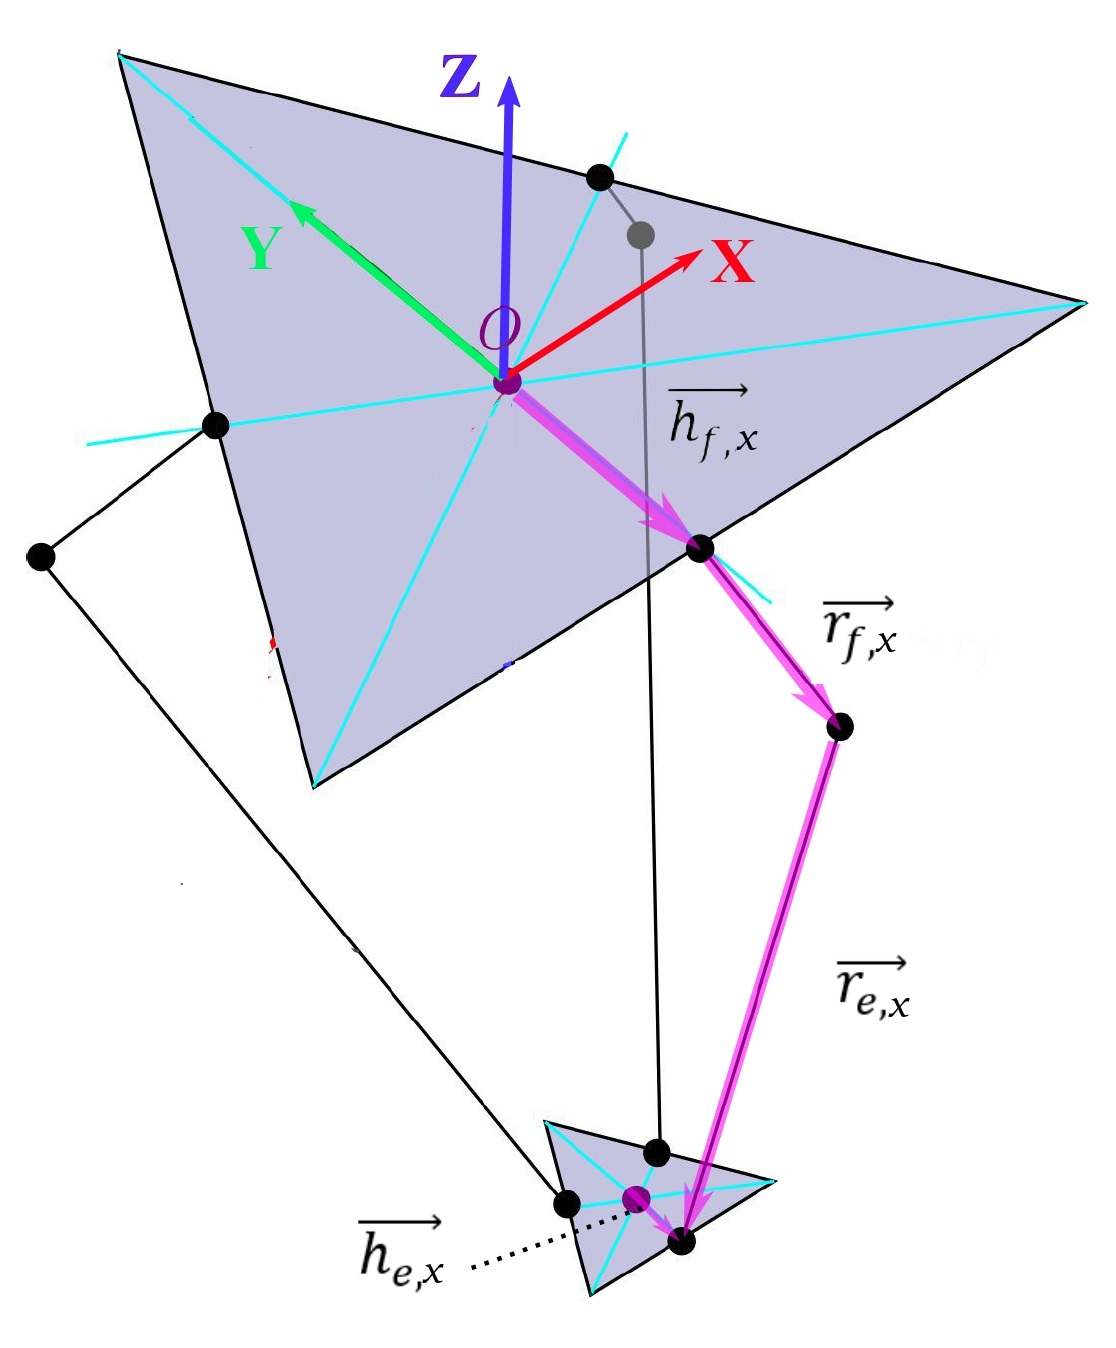
\includegraphics[width=0.7\linewidth]{Main/Chapter4/Images4/DIBUJO16.jpg}
            \caption{Vectorización de la cinemática inversa del método A}
            \label{fig:ANEXO_MA_C_POS_4}
        \end{figure}

        Se tiene conocimiento de las posiciones de todos los puntos sobre el efector, a causa de que se sabe posición del centroide del efector final  $E_{0} \left( x_{0},y_{0},z_{0} \right)$, la base fija es paralela al efector y además estas dos últimas partes mecánicas mencionadas tienen la misma orientación. Por lo tanto, se conocen las coordenadas de las juntas esféricas  $E_{i}$  que unen los antebrazos con el efector y a su vez los vectores $\overrightarrow{h_{e,x}}$ que representan la posición de las juntas esféricas  $E_{i}$ con respecto al centroide del efector.
        
        Con respecto a los vectores $\overrightarrow{r_{e,x}}$ , que representa los antebrazos, solo se conoce el punto final $E_{i}$ , que coincide con las posiciones de cada junta esférica unida al efector. Entonces, la orientación de cada vector  $\overrightarrow{r_{e,x}}$  , en cada uno de las 3 cadenas, está restringida por esferas con centros en las juntas esféricas $E_{i}$  con radio equivalente al largo del antebrazo $r_{e}$.
             \newpage

        En cuanto a los vectores $\overrightarrow{r_{f,x}}$  solo se conocen sus puntos iniciales $F_{i}$, que coinciden con la posición de cada actuador $i= \{ 1,2,3 \}$, sobre la base fija. Por otro lado, los actuadores son simplificados como juntas revolutas, por ende, restringen a cada uno de los vectores  $\overrightarrow{r_{f,x}}$ a moverse en un plano que contiene un punto en la posición del actuador  $F_{i}$ y un vector  $\overrightarrow{h_{f,x}}$. Las restricciones anteriores traen como consecuencia que las coordenadas de los puntos finales de vector  $\overrightarrow{r_{f,x}}$, es decir su extremo, estén sobre circunferencias Como se aprecia en la figura \ref{fig:ANEXO_MA_C_POS_4}.
        
        Finalmente, para obtener los ángulos de los actuadores  $\left(  \theta _{1}, \theta _{2}, \theta _{3} \right)$  , se calcula las intersecciónes\ entre las circunferencias formadas por el punto final de   $\overrightarrow{r_{f,x}}$  (con centro en  $F_{i}$ y de radio  $r_{f}$) y la esfera formada por el vector  $\overrightarrow{r_{e,x}}$ (con centro en  $E_{i}$ y de radio $r_{e}$) para cada cadena cinemática  $i= \{ 1,2,3 \}$. Esta intersección no es más que la junta esférica  $J_{i}$, recordando que la función de estas es unir los brazos con los antebrazos. Una vez obtenida la posición de las 3 juntas $J_{i}$, con álgebra simple se pueden obtener los valores de los ángulos $\left(  \theta _{1}, \theta _{2}, \theta _{3} \right)$.
        
        Como antes se ha mencionado, el primer paso para encontrar la configuración del espacio articular  $\left(  \theta _{1}, \theta _{2}, \theta _{3} \right)  $ es calcular las posiciones de las juntas $J_{i}$. Se empieza por la junta  $J_{1}$ que esta sobre el plano $YZ$ de nuestro sistema de referencia local. Se puede captar en la figura \ref{fig:ANEXO_MA_C_POS_5} que la intersección de la esfera y el plano $YZ$ es una circunferencia con centro en el punto $E^{'}_{1}$ y de radio $\overline{E^{'}_{1}J_{1}}$ . El punto $E^{'}_{1}$ es la proyección de  $E_{1}$  en el plano $YZ$.
        
        \begin{figure}[htb]
            \centering
            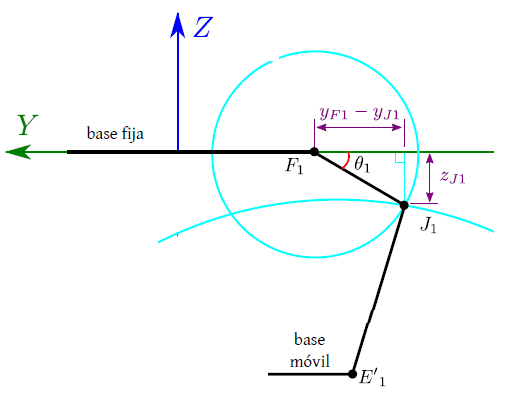
\includegraphics[width=0.9\linewidth]{Main/Chapter4/Images4/DIBUJOA11.png}
            \caption{Visualización plano YZ para representar la intersección de los 2 círculos en el punto $J_1$ para la solución de la cinemática inversa en el método A}
            \label{fig:ANEXO_MA_C_POS_5}
        \end{figure}
     
     \newpage

        El punto  $E_{1}$  que se usa para determinar el centro de la circunferencia $E'_{1}$  gracias a su proyección en el plano $YZ$, se calcula a partir de geometría simple de un triángulo equilátero de lado $e$ y de posición del centroide  $E_{0} \left( x_{0},y_{0},z_{0} \right)$  equivalente a la del efector final:
        
        \vspace{-1em}
        \begin{align*}
            &E_0E_1=\frac{e}{2}tan30=\frac{e}{2\sqrt{3}}\\
            &E_{1} \left( x_{0},y_{0}-\frac{e}{2\sqrt{3}},z_{0} \right) \Longrightarrow E'_{1} \left( 0,y_{0}-\frac{e}{2\sqrt{3}},z_{0} \right)
        \end{align*}


        El radio  $\overline{E^{'}_{1}J_{1}}$ de la circunferencia formada por la proyección del antebrazo en el plano $YZ$, se puede calcular por medio del teorema de pitagoras donde:
        
        \begin{align*}
            &E_1E'_1=x_0\\
            &\Longrightarrow E'_1J_1=\sqrt{E_1{J_1}^{2} - E_1{E'_1}^{2}} = \sqrt{{r_e}^{2}-{x_0}^{2}}
        \end{align*}
        
        
        \begin{figure}[htb]
            \centering
            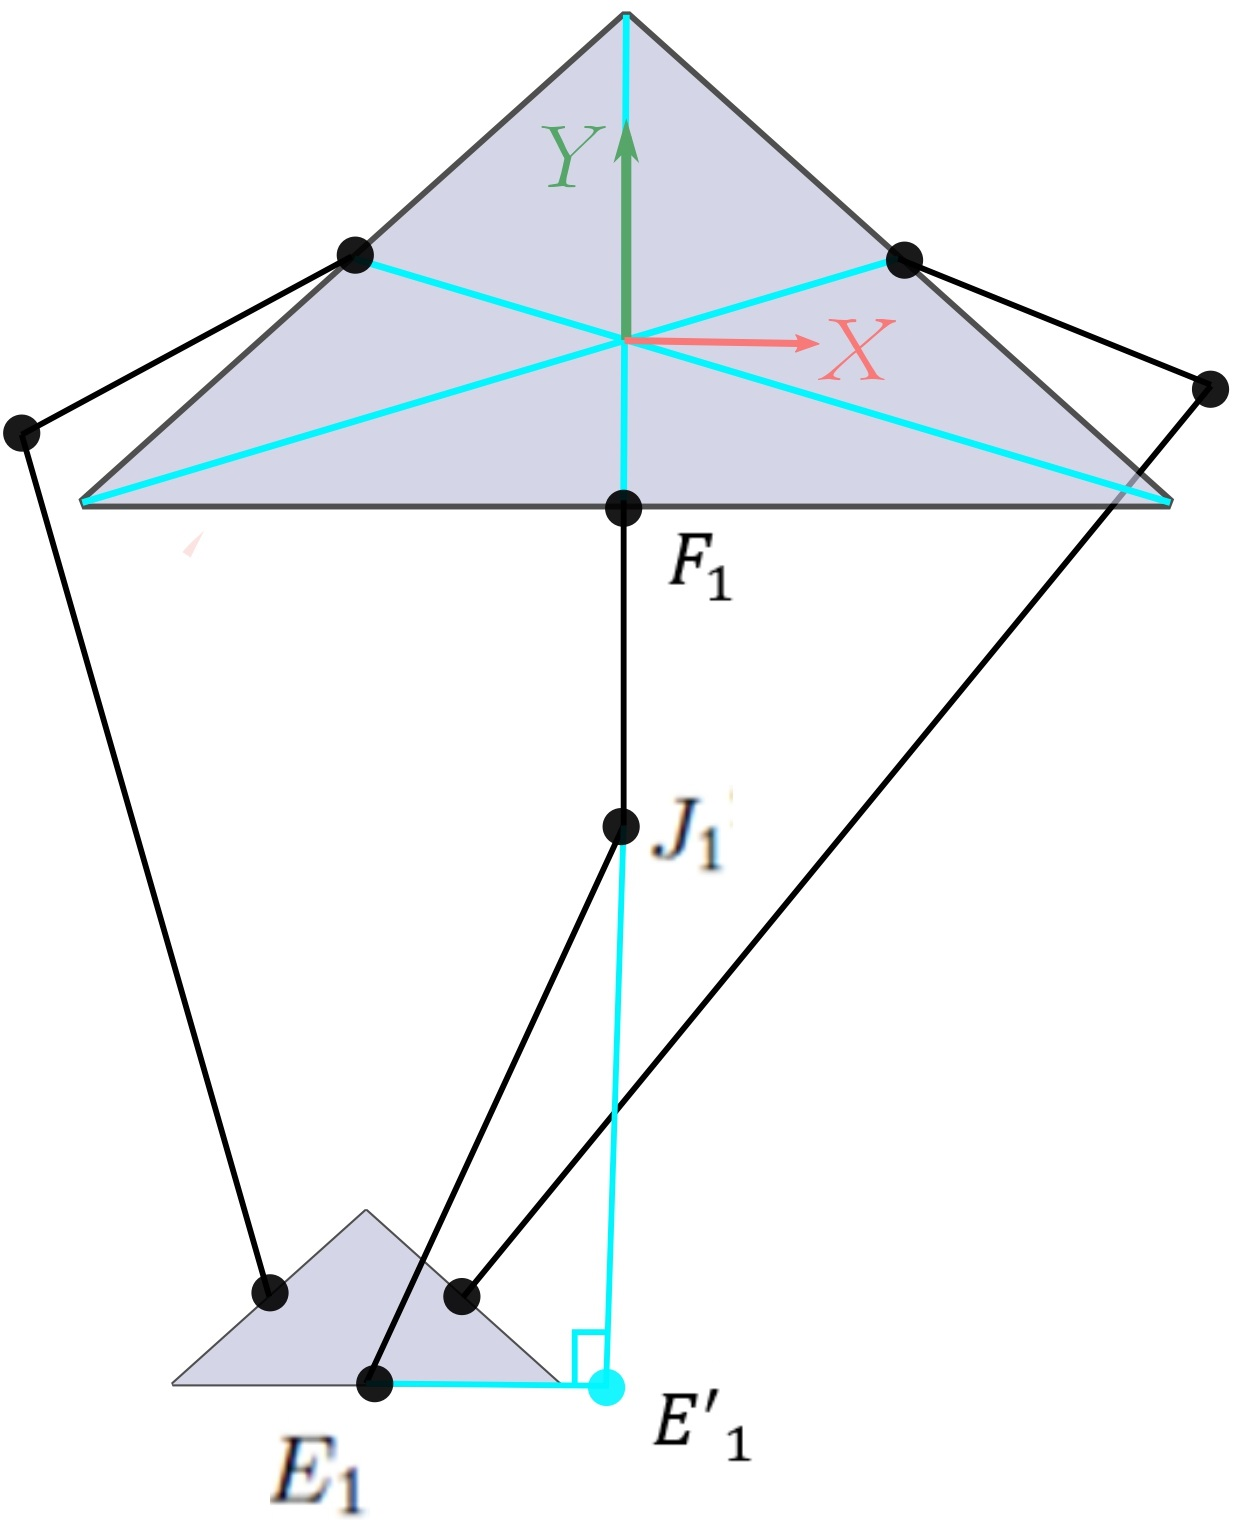
\includegraphics[width=0.7\linewidth]{Main/Chapter4/Images4/DIBUJO12.JPG}
            \caption{Proyección del punto $E_1$ sobre el plano YZ}
            \label{fig:ANEXO_MA_C_POS_7}
        \end{figure}      
        
     \newpage
         
       Resumiendo todo lo anterior, los centros de las circunferencias que intersectan la junta esférica $J_{1}$ son:
        \begin{center}
        \renewcommand{\arraystretch}{3.0}
        
            \begin{table}[H]
            \centering
            \begin{tabular}{c c } 
                 \hline
                 \textbf{Centros esferas}  & \textbf{Radio} \\ [0.1ex] 
                 \hline\hline
                         $\left(y_1,z_1\right)$ =
                        $F_1\left(y_{F_1}\,z_{F_1}\right)=\left(-\frac{f}{2\sqrt{3}},0\right)$\textit{} & 
                                                 $r_f$  \\ 
                \hline
                          $(y_2,z_2)$=
                          ${E^'}_{1}$ $(y_{{E^'}_1}$ $z_{{E^'}_1}$ $)=(y_0-\frac{e}{2\sqrt{3}},z_0)$ &
                          $r_2=\sqrt{{r_e}^2-{x_o}^2}$ \\
                \hline
            \end{tabular}
            \caption{Centro de esferas que representa las juntas en los puntos $E'_i$ y $F_i$}
            \label{tab:anexo_tabla_4}
            \end{table}
        \end{center}

       Ecuaciones cartesianas de las circunferencias son:
        \begin{equation*}
            \left\{ \begin{array}{c}
        	 \left( y-y_{1} \right) ^{2} + \left( z-z_{1} \right) ^{2}= r_{f}^{2}~\\
        	 \left( y-y_{2} \right) ^{2} + \left( z-z_{2} \right) ^{2}=r_{e}^{2}-x_{o}^{2}\\
        	\end{array}\right.
        \end{equation*}
        
        Desarrollando las ecuaciones anteriores y reordenando:
        \begin{equation*}
         \left\{ \begin{array}{c}
        	y^{2}+z^{2}-2yy_{1}-2zz_{1}= r_{f}^{2}-y_{1}^{2}-z_{1}^{2} ~ \left( 1 \right) \\
        	y^{2}+z^{2}-2yy_{2}-2zz_{2}=~ r_{e}^{2}-x_{o}^{2}-y_{2}^{2}-z_{2}^{2}  ~\left( 2 \right) \\
        	\end{array}\right.
        \end{equation*}
        
        Restando $(1)-(2)$
        
        \begin{equation*}
         -2y \left( y_{1}-y_{2} \right) -2z \left( z_{1}-z_{2} \right) = r_{f}^{2}-y_{1}^{2}-z_{1}^{2}- r_{e}^{2}+x_{o}^{2}+y_{2}^{2}+z_{2}^{2} 
        \end{equation*}
        
        Despejando $z$ en función de $y$:
        
        \begin{equation*}
         z=\frac{- \left( y_{1}-y_{2} \right) }{ \left( z_{1}-z_{2} \right) }\ast y+ \frac{r_{f}^{2}-y_{1}^{2}-z_{1}^{2}- r_{e}^{2}+x_{o}^{2}+y_{2}^{2}+z_{2}^{2}}{-2 \left( z_{1}-z_{2} \right)}
        \end{equation*}
        
        Donde:  
        \begin{align*}
             z&=a+by ~\left( 3 \right)\\
             b&=\frac{- \left( y_{1}-y_{2} \right) }{ \left( z_{1}-z_{2} \right) }~\\
             a&= \frac{r_{f}^{2}-y_{1}^{2}-z_{1}^{2}- r_{e}^{2}+x_{o}^{2}+y_{2}^{2}+z_{2}^{2}}{-2 \left( z_{1}-z_{2} \right) } \\ 
        \end{align*}
        
                \newpage

        Reemplazando  $z_{1}=0$, $y_{2}=y_{0}-\frac{e}{2\sqrt[]{3}}$  , $ ~y_{1}=-\frac{f}{2\sqrt[]{3}}$ :
        
        \begin{align*}
         b&=\frac{ \left( y_{1}-y_{2} \right) }{z_{2}}~ \\ 
         a&= \frac{x_{o}^{2}+y_{2}^{2}+z_{0}^{2}+r_{f}^{2}- r_{e}^{2}~-y_{1}^{2}}{2z_{0}} \\
         \Longrightarrow ~ a&= \frac{x_{o}^{2}+ \left( y_{0}-\frac{e}{2\sqrt[]{3}} \right) ^{2}+z_{0}^{2}+r_{f}^{2}- r_{e}^{2}~- \left( -\frac{f}{2\sqrt[]{3}} \right) ^{2}}{2z_{0}}
        \end{align*}
        
        Reemplazando la ecuación $(3)$ en $(1)$:
        
        \begin{equation*}
         \left( y-y_{1} \right) ^{2} + \left[  \left( a+by \right)  -z_{1} \right] ^{2}= r_{f}^{2} 
        \end{equation*}
        
        Desarrollando la ecuación anterior:
        
        \begin{align*}
         &\left( y^{2}-2yy_{1}+y_{1}^{2} \right) + \left( b^{2}y^{2}+2aby+a^{2} \right) -2 \left( a+by \right) z_{1}+ z_{1}^{2}=~r_{f}^{2}~\\
         \Longrightarrow ~~  & \left( b^{2}+1 \right) y^{2}+ \left( -2y_{1}+2ab \right) y + \left( y_{1}^{2}+a^{2}-r_{f}^{2} \right) +z_{1} \left( -2 \left( a+by \right) +z_{1}~ \right) =0~  \left( 4 \right)
        \end{align*}
        
        La solución y para la ecuación cuadrática $(4)$ está dada por:
        
        \begin{equation*}
             y= \frac{- \left( 2ab-2y_{1} \right)   \pm \sqrt[]{d}}{2 \left( b^{2}+1 \right) }
        \end{equation*}
        
        Se aprecian dos soluciones, donde se elige la $y=\frac{- \left( 2ab-2y_{1} \right) -\sqrt[]{d}}{2 \left( b^{2}+1 \right) }$ para que el ángulo entre el brazo y el antebrazo no exceda los 180$ ^{\circ} $.
        
        El discriminante $d$ es:
        
        \begin{equation*}
             d= \left( 2ab-2y_{1} \right) ^{2}-4\ast \left( b^{2}+1 \right) \ast \left[  \left( y_{1}^{2}+a^{2}-r_{f}^{2} \right) +z_{1}\ast \left( -2 \left( a+by \right) +z_{1}\right)  \right]
        \end{equation*}
        
        Reemplazando $z_{1}=0$ y reordenando:
        
        \begin{align*}
         d&= \left( 2ab-2y_{1} \right) ^{2}-4\ast \left( b^{2}+1 \right) \ast \left( y_{1}^{2}+a^{2}-r_{f}^{2} \right) \\
         \Longrightarrow d&=4 \left[ ~ \left( ab-y_{1} \right) ^{2}- \left( b^{2}+1 \right) \ast \left( y_{1}^{2}+a^{2}-r_{f}^{2} \right)  \right]  \\
         \Longrightarrow d&=4 \left[  \left( ~a^{2}b^{2}-2aby_{1}+~y_{1}^{2} \right) + \left( -b^{2}y_{1}^{2}-b^{2}a^{2}+b^{2}r_{f}^{2} \right) - \left( y_{1}^{2}+a^{2}-r_{f}^{2} \right)  \right]  \\
         \Longrightarrow d&=4 \left[ -a^{2}-2aby_{1}-b^{2}y_{1}^{2}+b^{2}r_{f}^{2}+r_{f}^{2} \right]  \\
         \Longrightarrow d&=4 \left[ - \left( a+by_{1} \right) ^{2}+ \left( b^{2}+1 \right) r_{f}^{2} \right]  \\ 
        \end{align*}
        
        \newpage
        
        Por lo tanto, la solución y para el sistema de ecuaciones de las circunferencias es:
        
        \begin{align*}
         y&= \frac{- \left( 2ab-2y_{1} \right) -\sqrt[]{4 \left[ - \left( a+by_{1} \right) ^{2}+ \left( b^{2}+1 \right) r_{f}^{2} \right] }}{2 \left( b^{2}+1 \right) } \\
         \Longrightarrow y&= \frac{ \left( y_{1}-ab \right) -\sqrt[]{ \left[ - \left( a+by_{1} \right) ^{2}+ \left( b^{2}+1 \right) r_{f}^{2} \right] }}{ \left( b^{2}+1 \right) } \\ 
        \end{align*}
        
        Por lo tanto, la solución del sistema de ecuaciones es:

        \begin{equation*}
         J_{1}= \left( x_{J_{1}},y_{J_{1}},z_{J_{1}} \right) = \left( 0,y,a+by \right) 
        \end{equation*}
        
        \begin{equation*}
         J_{1}= \left( 0,\frac{ \left( y_{1}-ab \right) -\sqrt[]{ \left[  \left( a+by_{1} \right) ^{2}+ \left( b^{2}+1 \right) r_{f}^{2} \right] }}{ \left( b^{2}+1 \right) },a+b\frac{ \left( y_{1}-ab \right) -\sqrt[]{ \left[  \left( a+by_{1} \right) ^{2}+ \left( b^{2}+1 \right) r_{f}^{2} \right] }}{ \left( b^{2}+1 \right) } \right)
        \end{equation*}
        
        Finalmente, se determina el ángulo $\theta _{1}$ por medio del triángulo rectángulo formado en el brazo y la proyección del mismo en el plano $XY$, como se ilustra en la figura \ref{fig:ANEXO_MA_C_POS_5}:
        

        \begin{equation*}
         \theta _{1}=\arctan  \left( ~\frac{z_{J_{1}}}{y_{F_{1}}-y_{J_{1}}} \right)  
        \end{equation*}

        
        Donde  $y_{F_{1}}$ se obtiene de la geometría básica que tiene la base fija (figura \ref{fig:ANEXO_MA_C_POS_9}):

        \begin{equation*}
            F_1(0,-\frac{f}{2\sqrt{3}},0)
        \end{equation*}
        
        \begin{figure}[htb]
            \centering
            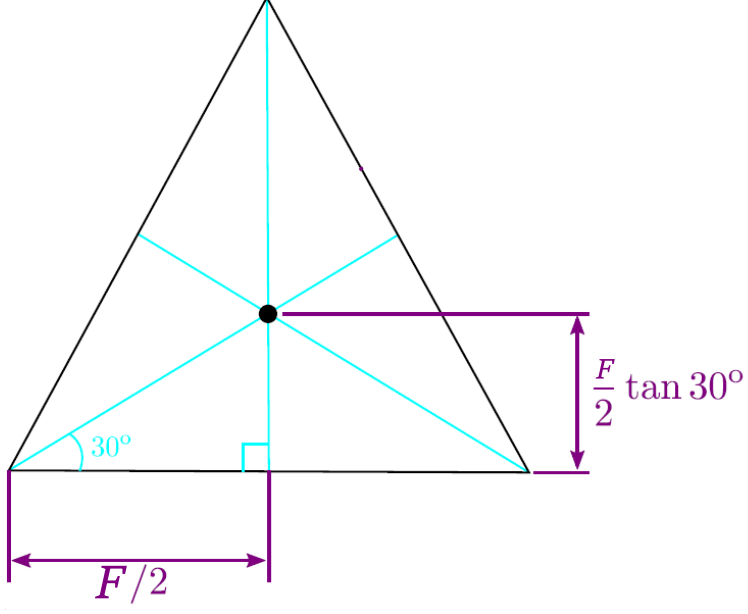
\includegraphics[width=0.5\linewidth]{Main/Chapter4/Images4/DIBUJO15.PNG}
            \caption{Vista superior de la base fija}
            \label{fig:ANEXO_MA_C_POS_9}
        \end{figure}
        
        \newpage
        
        Aprovechando la simetría del robot delta, se utiliza el mismo método empleado en la solución de  $\theta _{1}$  para los ángulos  $\theta _{2}$  y  $\theta _{3}$ . Para calcularlos, se utilizan matrices de rotación con un ángulo de rotación de 120$ ^{\circ} $  para la cadena cinemática con el actuador 2 y de 240$ ^{\circ} $  para la cadena cinemática con el actuador 3. Estas matrices giran el sistema de referencia local en 120$ ^{\circ} $  y 240$ ^{\circ} $  grados como se observa en la figura \ref{fig:ANEXO_MA_C_POS_10}:
        
        \begin{figure}[htb]
            \centering
            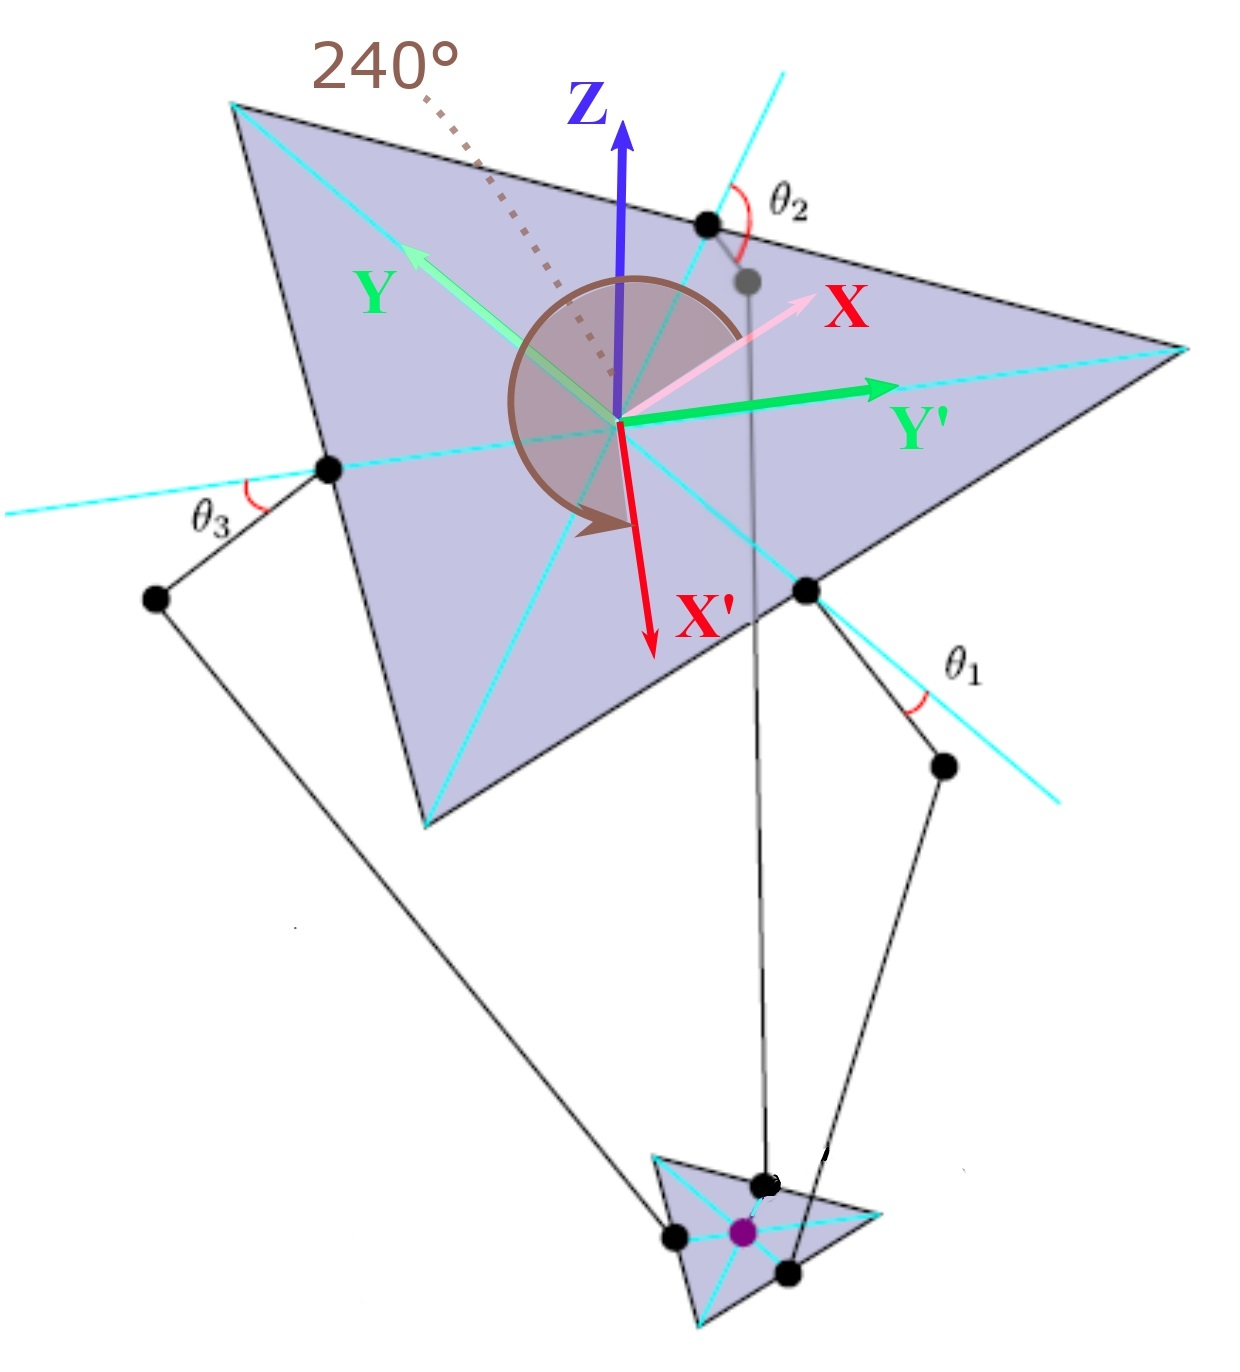
\includegraphics[width=0.9\linewidth]{Main/Chapter4/Images4/DIBUJO17.jpg}
            \caption{Representación de la rotación del sistema coordenado $XYZ$ en $240^{\circ}$ para la solución de la cinemática inversa en el método A}
            \label{fig:ANEXO_MA_C_POS_10}
        \end{figure}
     
     \newpage
        
        
    \subsection{Modelación cinemática de velocidad}\label{anexomodelacionvelocidadmetodoa}
            \subsubsection{Vectorización y ángulos de juntas}
            
        La figura \ref{f:Cap4_Metodo_A_Modelacion_Cinematica_Posicion_8} define los ángulos de articulación asociados con la extremidad  $i$, donde  $\overrightarrow{p}$  es el vector de posición del centroide de la plataforma móvil, $\theta _{1i}$  se mide desde el eje $x_{i}$  hasta $\overrightarrow{A_{i}B_{i}}$ ,$\theta _{2i}$  se define desde la línea extendida de $\overrightarrow{A_{i}B_{i}}$  hasta la línea definida por la intersección del plano del paralelogramo y el plano $x_{i}-z_{i}$ y $\theta _{3i}$  se mide desde la dirección $y_{i}$ hasta $\overrightarrow{B_{i}C_{i}}$ . En general, hay 9 ángulos articulares, $\theta _{1i}$, $\theta _{2i}$ y $\theta _{3i}$ para $i= \{  1, 2, 3 \}$, asociados con el manipulador. Los ángulos de los actuadores son $\theta _{11}$ ,$\theta _{21}$ y $\theta _{31}$ .
        
        Se puede escribir una ecuación de cierre de bucle para cada extremidad vectorialmente:
        
        \begin{equation}
             \overrightarrow{A_{i}B_{i}}+ \overrightarrow{B_{i}C_{i}}~~ =\overrightarrow{OP}~ +\overrightarrow{~PC_{i}} -\overrightarrow{OA_{i}~}
             \label{eq:modelacion_cine_vel_metodoa_anexo_1}
        \end{equation}
        
        Reescribiendo \ref{eq:modelacion_cine_vel_metodoa_anexo_1} en el marco de coordenadas  $A_{i}$ –    $x_{i}y_{i}z_{i}$ conduce a la siguiente representación matricial:
        
        \begin{equation}
                 a \left[ \begin{matrix}
                cos~ \theta _{1i}\\
                0\\
                sin~ \theta _{1i}\\
                \end{matrix}
                 \right] +b \left[ \begin{matrix}
                sin~ \theta _{3i}cos⁡ \left(  \theta _{1i}+ \theta _{2i} \right) \\
                cos~ \theta _{3i}\\
                sin~ \theta _{3i}sin \left(  \theta _{1i}+ \theta _{2i} \right) \\
                \end{matrix}
                 \right] = \left[ \begin{matrix}
                c_{xi}\\
                c_{yi}\\
                c_{zi}\\
                \end{matrix} \right] 
                \label{eq:modelacion_cine_vel_metodoa_anexo_2}
        \end{equation}
        
        \begin{equation}
                    \left[ \begin{matrix}
                    c_{xi}\\
                    c_{yi}\\
                    c_{zi}\\
                    \end{matrix}
                     \right] = \left[ \begin{matrix}
                    \cos  \phi _{i}  &  \sin  \phi _{i}  &  0\\
                    -sin \phi _{i}  &  \cos  \phi _{i}  &  0\\
                    0  &  0  &  1\\
                    \end{matrix}
                     \right]  \left[ \begin{matrix}
                    p_{x}\\
                    p_{y}\\
                    p_{z}\\
                    \end{matrix}
                     \right] +  \left[ \begin{matrix}
                    h\\
                    0\\
                    0\\
                    \end{matrix}
                     \right] - \left[ \begin{matrix}
                    r\\
                    0\\
                    0\\
                    \end{matrix}
                     \right] 
                \label{eq:modelacion_cine_vel_metodoa_anexo_3}
        \end{equation}

        \begin{figure}[htb]
            \centering
            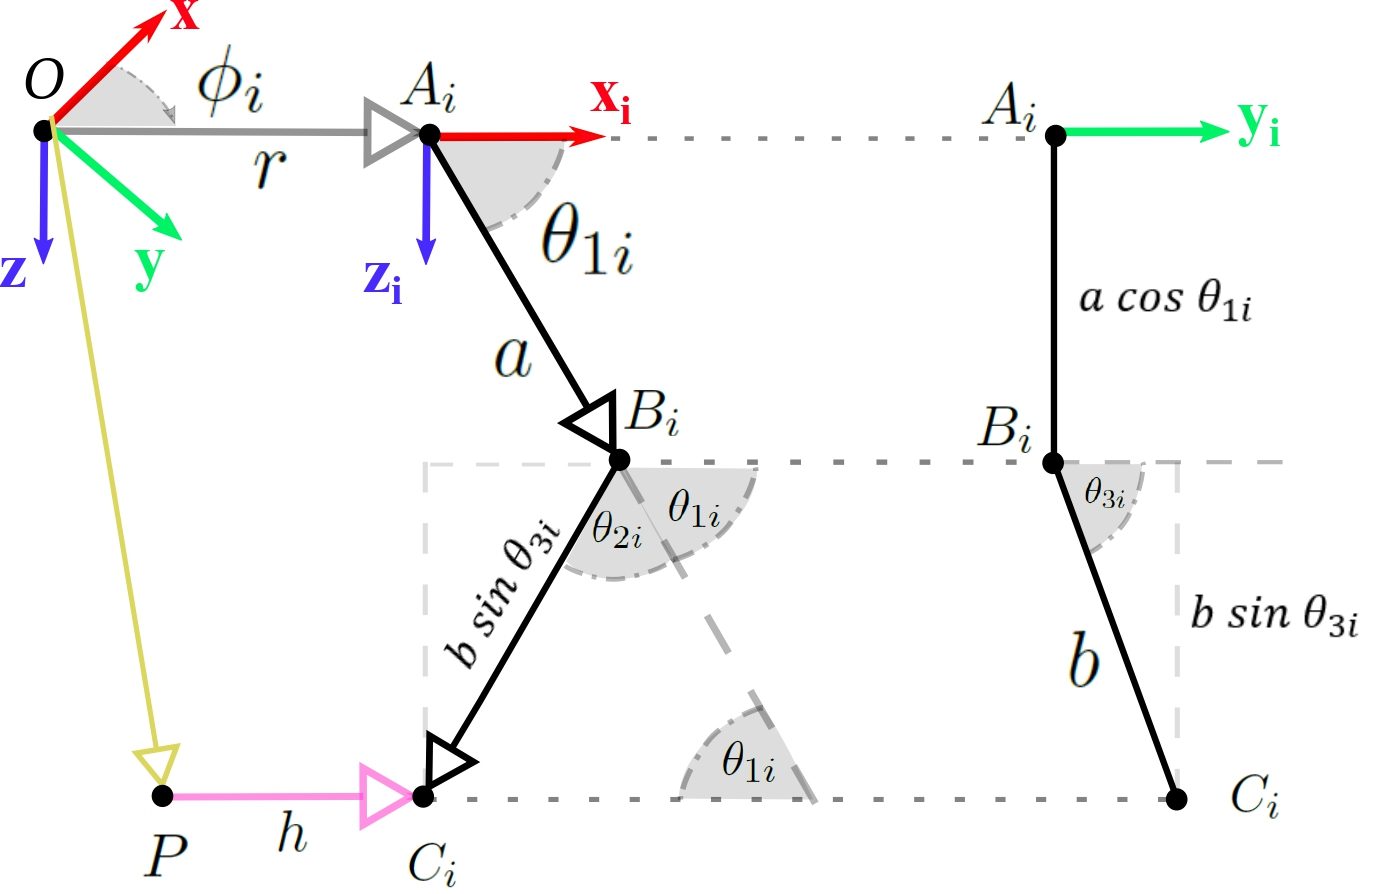
\includegraphics[width=0.9\linewidth]{Main/Chapter4/Images4/DIBUJO22.jpg}
            \caption{Vectorización y ángulos interiores para la solución de la cinemática de velocidad del método A}
            \label{fig:ANEXO_MA_C_vel_1}
        \end{figure}
     
        \newpage


        La figura \ref{fig:ANEXO_MA_C_vel_1} denota la posición del punto  $C_{i}$  en relación con el marco de coordenadas  $A_{i}$ – $x_{i}y_{i}z_{i}$ ,$a$  y  $b$ son las longitudes de los enlaces $\overrightarrow{A_{i}B_{i}}$ , y  $\overrightarrow{B_{i}C_{i}}$  respectivamente y $\overrightarrow{p}= \left[ p_{x},p_{y},p_{z} \right] ^{T}$  es el vector de posición del punto $P$   relativo al sistema de coordenadas $O$ – $xyz$.
        
        El ángulo $\theta _{3i}$  se calcula resolviendo la segunda fila de la ecuación \ref{eq:modelacion_cine_vel_metodoa_anexo_2}:

        \begin{equation}
            \theta _{3i}= \cos ^{-1}\frac{c_{yi}}{b} 
            \label{eq:modelacion_cine_vel_metodoa_anexo_3}
        \end{equation}
        
        Con  $\theta _{3i}$  determinado, se genera una ecuación con $\theta _{2i}$ como la única incógnita, sumando los cuadrados de  $c_{xi}$ ,  $c_{yi}$  y  $c_{zi}$ en la ecuación \ref{eq:modelacion_cine_vel_metodoa_anexo_2} aplicando la norma a los vectores:
        \vspace{-1em}
        
      \begin{equation*}
                      &\left \Vert a
            \left[ \begin{matrix}
            cos~ \theta _{1i}\\
            0\\
            sin~ \theta _{1i}\\
            \end{matrix}\right] +b \left[ \begin{matrix}
            sin~ \theta _{3i} cos⁡ \left(  \theta _{1i}+ \theta _{2i} \right) \\
            cos~ \theta _{3i}\\
            sin~ \theta _{3i}sin \left(  \theta _{1i}+ \theta _{2i} \right) \\
            \end{matrix}
             \right] ~~ \right \Vert =~~ \left \Vert ~~~ \left[ \begin{matrix}
            c_{xi}\\
            c_{yi}\\
            c_{zi}\\
            \end{matrix}
             \right] ~~~ \right \Vert \\
      \end{equation*}  
              \vspace{-1em}
     \begin{align*}
             \Longrightarrow & \left( a cos~ \theta _{1i}+b sin~ \theta _{3i}~cos⁡ \left(  \theta _{1i}+ \theta _{2i} \right)  \right) ^{2}+\\
              &\left( b cos~ \theta _{3i} \right) ^{2}+ \left( a sin~ \theta _{1i}+b sin~ \theta _{3i}sin \left(  \theta _{1i}+ \theta _{2i} \right)  \right) ^{2} = c_{xi}^{2}+c_{yi}^{2}+c_{zi}^{2}\\
             \Longrightarrow &  \left[ a^{2}cos^{2}\theta _{1i}+\2ab cos~ \theta _{1i}sin~ \theta _{3i}\cos  \left(  \theta _{1i}+ \theta _{2i} \right) +b^{2}sin ^{2}~ \theta _{3i} cos ^{2}⁡ \left(  \theta _{1i}+ \theta _{2i} \right) \right] +\\
             &\left[ b^{2}~cos^{2} \theta _{3i} \right] + \left[ a^{2}~sin^{2} \theta _{1i}+2ab~sin~ \theta _{1i}sin~ \theta _{3i}sin \left(  \theta _{1i}+ \theta _{2i} \right) +b^{2}sin^{2}  \theta _{3i} sin^{2}  \left(  \theta _{1i}+ \theta _{2i} \right) \right]=\\
             &c_{xi}^{2}+c_{yi}^{2}+c_{zi}^{2}\\
             \Longrightarrow & a^{2} \left( cos^{2} \theta _{1i}+~sin^{2} \theta _{1i} \right) +b^{2}sin^{2} ~ \theta _{3i} \left( \cos^{2}   \left(  \theta _{1i}+ \theta _{2i} \right)+\sin^{2}   \left(  \theta _{1i}+ \theta _{2i} \right)\right) +\\
             &2 ab sin~ \theta _{3i} \left( ~cos~ \theta _{1i}\cos  \left(  \theta _{1i}+ \theta _{2i} \right) +sin~ \theta _{1i}\sin  \left(  \theta _{1i}+ \theta _{2i} \right)  \right) +b^{2}~cos^{2} \theta _{3i}= c_{xi}^{2}+c_{yi}^{2}+c_{zi}^{2}
        \end{align*}
        
        Utilizando las siguientes propiedades trigonométricas:
        \begin{gather*}
            \cos^{2}~ \theta _{1i}+~sin^{2}~ \theta _{1i}=1\\
            \cos^{2}  \left(  \theta _{1i}+ \theta _{2i} \right)+\sin ^{2} \left(  \theta _{1i}+ \theta _{2i} \right) =1 \\
            \cos \theta _{1i}\cos  \left(  \theta _{1i}+ \theta _{2i} \right) +sin~ \theta _{1i}sin \left(  \theta _{1i}+ \theta _{2i} \right) =cos⁡  \left(  \theta _{1i}- \left(  \theta _{1i}+ \theta _{2i} \right)  \right) = cos⁡  \left(  \theta _{2i} \right)
        \end{gather*}

        Reemplazando:
        \begin{equation*}
         \Longrightarrow a^{2}+b^{2}sin^{2} ~ \theta _{3i}+ 2 ab sin~ \theta _{3i}\cos  \theta _{2i}+b^{2}~cos^{2} ~ \theta _{3i}= c_{xi}^{2}+c_{yi}^{2}+c_{zi}^{2} 
        \end{equation*}
        
        Donde se sabe que:
        \begin{equation*}
            \left( sin^{2}~ \theta _{3i}+~cos^{2} \theta _{3i} \right) =1
        \end{equation*}
        
        Entonces:
        \begin{equation*}
            a^{2}+b^{2}+ 2 ab sin~ \theta _{3i}\cos  \theta _{2i}+b^{2}= c_{xi}^{2}+c_{yi}^{2}+c_{zi}^{2}
        \end{equation*}
        
        Despejando  $\theta _{2i}$:
                \vspace{-0.2em}
        \begin{equation}
          \theta _{2i}=\cos ^{-1} \left( \frac{c_{xi}^{2}+c_{yi}^{2}+c_{zi}^{2}- a^{2}-b^{2}~}{2 ab sin~ \theta _{3i}} \right) 
        \end{equation}
        
        Con  $\theta _{3i}$  y  $\theta _{2i}$  determinados, solo queda un par de ecuaciones con $\theta _{1i}$  como la única incógnita que desde la ecuación \ref{eq:modelacion_cine_vel_metodoa_anexo_2}. Por lo tanto, es posible resolver el valor de $ \theta _{1i}$.

\newpage


        \subsubsection{Jacobiano}
            Con referencia a la figura \ref{fig:ANEXO_MA_C_vel_1}, una ecuación de cierre de bucle para una extremidad $i$ sistema de referencia $A_{i}$ – $ x_{i}y_{i}z_{i}$  se puede escribir como:
            
            \begin{equation}
                 \overrightarrow{OP}+\overrightarrow{~PC_{i}} =\overrightarrow{OA_{i}}+\overrightarrow{A_{i}B_{i}}+\overrightarrow{B_{i}C_{i}}
            \label{eq:jac_met_a_anex_1}
            \end{equation}
            
            Al diferenciar vectorialmente la ecuación \ref{eq:jac_met_a_anex_1} con respecto a el tiempo:
            
            \begin{equation*}
                 \dot{\overrightarrow{OP}}+\dot{\overrightarrow{~PC_{i}}}= \dot{\overrightarrow{OA_{i}}}+ \dot{\overrightarrow{A_{i}B_{i}}}+ \dot{\overrightarrow{B_{i}C_{i}}} 
            \end{equation*}
            
            Donde  $\dot{\overrightarrow{~PC_{i}}}= \dot{\overrightarrow{OA_{i}}}=0$ , entonces:
            
            \begin{equation}
                 \overrightarrow{v_{p}}= \overrightarrow{ \omega _{1i}}~\times~~\overrightarrow{a_{i}}+  \overrightarrow{ \omega _{2i}}~\times~\overrightarrow{b_{i}}
            \label{eq:jac_met_a_anex_2}
            \end{equation}
            
            Donde  $ \overrightarrow{v_{p}}= \left[ v_{px},v_{py},v_{pz} \right] ^{T}$ es la velocidad lineal de la plataforma móvil, $\overrightarrow{a_{i}}= \overrightarrow{A_{i}B_{i}}$, $ \overrightarrow{b_{i}}=\overrightarrow{~B_{i}C_{i}}$  y   $\overrightarrow{ \omega _{ji}}$  es la velocidad angular del eslabón $j$ de la cadena cinemática $i$. Para eliminar $\omega _{2i}$  es necesario hacer un producto punto en ambos lados de la ecuación \ref{eq:jac_met_a_anex_2} por un vector unitario  $ \widehat{b_{i}} $ . Por lo tanto:
            \vspace{-0.5em}
            \begin{align*}
                 \widehat{b_{i}} \cdot  \overrightarrow{v_{p}}&= \widehat{b_{i}}  \cdot  \left( ~\overrightarrow{ \omega _{1i}}~\times~~\overrightarrow{a_{i}}~~~+  \overrightarrow{ \omega _{2i}}~\times~\overrightarrow{b_{i}} \right) ~~~ \\ 
                 \Longrightarrow ~\widehat{b_{i}}  \cdot  \overrightarrow{v_{p}}&= \widehat{b_{i}}  \cdot  \left( ~\overrightarrow{ \omega _{1i}}~\times~~\overrightarrow{a_{i}}~ \right)  +\widehat{b_{i}}  \cdot  \left( ~\overrightarrow{ \omega _{2i}}~\times~\overrightarrow{b_{i}} \right) ~~~  \\ 
                 \Longrightarrow ~\widehat{b_{i}}  \cdot  \overrightarrow{v_{p}}&= \overrightarrow{ \omega _{1i}} \cdot  \left( ~\overrightarrow{a_{i}}~\times~~\widehat{b_{i}}~ \right)  +\overrightarrow{ \omega _{2i}} \cdot  \left( \overrightarrow{b_{i}}~\times~\widehat{b_{i}}~ \right) ~  \\
                 \Longrightarrow ~\widehat{b_{i}}  \cdot  \overrightarrow{v_{p}}&= \overrightarrow{ \omega _{1i}} \cdot  \left( ~\overrightarrow{a_{i}}~\times~~\widehat{b_{i}} \right) ~  \\
                 \Longrightarrow ~~\widehat{b_{i}} \cdot \overrightarrow{v_{p}}&= \widehat{b_{i}} \cdot  \left( ~\overrightarrow{ \omega _{1i}}~\times~\overrightarrow{a_{i}} \right)
            \end{align*}
            
            Por lo tanto, la igualdad que se utiliza para calcular el jacobiano es: 
            \begin{equation}
                \widehat{b_{i}} \cdot \overrightarrow{v_{p}}&= \widehat{b_{i}} \cdot  \left( ~\overrightarrow{ \omega _{1i}}~\times~\overrightarrow{a_{i}} \right)
                \label{eq:jac_met_a_anex_3}
            \end{equation}
            
            El vector unitario del vector  $\overrightarrow{b_{i}}$ es calculado con la siguiente expresión:
            
            \begin{equation*}
                \widehat{b_{i}}&=\frac{\overrightarrow{b_{i}}}{ \Vert \overrightarrow{b_{i}} \Vert }=\frac{\overrightarrow{b_{i}}}{b}= \left[ \begin{matrix}
                sin~ \theta _{3i}cos⁡ \left(  \theta _{1i}+ \theta _{2i} \right) \\
                cos~ \theta _{3i}\\
                sin~ \theta _{3i}sin \left(  \theta _{1i}+ \theta _{2i} \right) \\
                \end{matrix}
                 \right]  
            \end{equation*}
            
            Al reescribir los vectores de la ecuación \ref{eq:jac_met_a_anex_3} en el marco de coordenadas  $A_{i}$–$x_{i}y_{i}z_{i}$ conduce a:
            \begin{align*}
                            \overrightarrow{a_{i}}= a \left[ \begin{matrix}
                cos \theta _{1i}\\
                0\\
                sin \theta _{1i}\\
                \end{matrix}
                 \right] ;&\overrightarrow{b_{i}}=b \left[ \begin{matrix}
                sin \theta _{3i}cos⁡ \left(  \theta _{1i}+ \theta _{2i} \right) \\
                cos \theta _{3i}\\
                sin \theta _{3i}sin \left(  \theta _{1i}+ \theta _{2i} \right) \\
                \end{matrix}\right];&\overrightarrow{ \omega _{1i}}= \left[ \begin{matrix}
                0\\
                -\dot{ \theta _{1i}}\\
                0\\
                \end{matrix}
                 \right];&\overrightarrow{v_{p}}= \left[ \begin{matrix}
                v_{px}\cos  \phi _{i}+v_{py}\sin  \phi _{i}\\
                -v_{px}\sin  \phi _{i}+v_{py}\cos  \phi _{i}\\
                v_{pz}\\
                \end{matrix} \right]
            \end{align*}
            
            El signo negativo en la segunda fila de  $\overrightarrow{ \omega _{1i}}$ es solo una cuestión de convención. 

            \newpage
            
            Calculando  $\widehat{b_{i}} \cdot \overrightarrow{v_{p}}$,  sustituyendo los valores $\widehat{b_{i}}$ y  $\overrightarrow{v_{p}}$:

            \begin{align*}
                  \widehat{b_{i}} \cdot \overrightarrow{v_{p}} &= \left[ \begin{matrix}
                    sin~ \theta _{3i}cos⁡ \left(  \theta _{1i}+ \theta _{2i} \right) \\
                    cos~ \theta _{3i}\\
                    sin~ \theta _{3i}sin \left(  \theta _{1i}+ \theta _{2i} \right) \\
                    \end{matrix}
                     \right]  \cdot  \left[ \begin{matrix}
                    v_{px}\cos  \phi _{i}+v_{py}\sin  \phi _{i}\\
                    -v_{px}\sin  \phi _{i}+v_{py}\cos  \phi _{i}\\
                    v_{pz}\\
                    \end{matrix}
                     \right]\\
                 &= \left[  \left( sin~ \theta _{3i}cos⁡ \left(  \theta _{1i}+ \theta _{2i} \right)  \right) \ast \left( v_{px}\cos  \phi _{i}+v_{py}\sin  \phi _{i} \right)  \right] +\\
                 ~~ &\left[  \left( cos~ \theta _{3i} \right) \ast \left( -v_{px}\sin  \phi _{i}+v_{py}\cos  \phi _{i} \right)  \right] +\\
                 ~~~&\left[  \left( sin~ \theta _{3i}sin \left(  \theta _{1i}+ \theta _{2i} \right)  \right) \ast \left( v_{pz} \right)  \right] \\
                 &= \left[ sin~ \theta _{3i}\cos  \left(  \theta _{1i}+ \theta _{2i} \right) \cos  \phi _{i}-cos  \theta _{3i}\sin  \phi _{i} \right] v_{px}+\\
                 ~~~&\left[ sin~ \theta _{3i}\cos  \left(  \theta _{1i}+ \theta _{2i} \right) \sin  \phi _{i}+ cos  \theta _{3i}\cos  \phi _{i} \right] v_{py}+\\ 
                 ~~~&\left[  \left( sin~ \theta _{3i}sin \left(  \theta _{1i}+ \theta _{2i} \right)  \right)  \right] v_{pz} \\
                 &=J_{ix}v_{px}+J_{iy}v_{py}+J_{iz}v_{pz} 
            \end{align*}
            
            Por lo tanto:
            \begin{equation}
                 \widehat{b_{i}} \cdot \overrightarrow{v_{p}} =J_{ix}v_{px}+J_{iy}v_{py}+J_{iz}v_{pz}
                                 \label{eq:jac_met_a_anex_5}
            \end{equation}
            
            Donde:
            \begin{align}
                  J_{ix}&=\cos  \left(  \theta _{1i}+ \theta _{2i} \right) sin~ \theta _{3i}\cos  \phi _{i}-cos  \theta _{3i}\sin  \phi _{i}~\\
                  J_{iy}&=\cos  \left(  \theta _{1i}+ \theta _{2i} \right) sin~ \theta _{3i}\sin  \phi _{i}+ cos  \theta _{3i}\cos  \phi _{i}~ \\
                  J_{iz}&=sin \left(  \theta _{1i}+ \theta _{2i} \right) sin~ \theta _{3i}~ 
                \end{align}
                
                Calculando $\widehat{b_{i}} \cdot  \left( ~\overrightarrow{ \omega _{1i}}~\times~\overrightarrow{a_{i}} \right)$, sustituyendo los valores $\overrightarrow{a_{i}}$, $\widehat{b_{i}}$, $\overrightarrow{ \omega _{1i}}$:
                
                \begin{align*}
                 &\widehat{b_{i}} \cdot  \left( ~\overrightarrow{ \omega _{1i}}~\times~\overrightarrow{a_{i}} \right)= \left[ \begin{matrix}
                sin~ \theta _{3i}cos⁡ \left(  \theta _{1i}+ \theta _{2i} \right) \\
                cos~ \theta _{3i}\\
                sin~ \theta _{3i}sin \left(  \theta _{1i}+ \theta _{2i} \right) \\
                \end{matrix}
                 \right]  \cdot   \left( ~ \left[ \begin{matrix}
                0\\
                -\dot{ \theta _{1i}}\\
                0\\
                \end{matrix}
                 \right] \times a \left[ \begin{matrix}
                cos~ \theta _{1i}\\
                0\\
                sin~ \theta _{1i}\\
                \end{matrix}
                 \right]  \right) \\
                &= \left[ \begin{matrix}
                sin~ \theta _{3i}cos⁡ \left(  \theta _{1i}+ \theta _{2i} \right) \\
                cos~ \theta _{3i}\\
                sin~ \theta _{3i}sin \left(  \theta _{1i}+ \theta _{2i} \right) \\
                \end{matrix}
                 \right]  \cdot  a \left[ \begin{matrix}
                -sin  \theta _{1i}\dot{ \theta _{1i}}\\
                0\\
                cos~ \theta _{1i}\dot{ \theta _{1i}}\\
                \end{matrix}
                 \right] \\
                 &=a~  \left( -sin  \theta _{3i}cos⁡ \left(  \theta _{1i}+ \theta _{2i} \right) sin  \theta _{1i}\dot{ \theta _{1i}} \right) + \left( sin~ \theta _{3i}sin \left(  \theta _{1i}+ \theta _{2i} \right) cos  \theta _{1i}\dot{ \theta _{1i}} \right)  \\
                 &=a~ \dot{ \theta _{1i}}sin~ \theta _{3i} \left( -\cos  \left(  \theta _{1i}+ \theta _{2i} \right) sin~ \theta _{1i}+sin \left(  \theta _{1i}+ \theta _{2i} \right) cos  \theta _{1i} \right) \\
                 &=a~ \dot{ \theta _{1i}}~sin~ \theta _{3i}~ \left( -\cos  \left(  \theta _{1i}+ \theta _{2i} \right) sin~ \theta _{1i}+sin \left(  \theta _{1i}+ \theta _{2i} \right) cos  \theta _{1i} \right) \\
                 &=a~ \dot{ \theta _{1i}}~sin~ \theta _{3i} sin \left(  \theta _{1i}+ \theta _{2i}- \theta _{1i} \right)\\
                 &=a~ \dot{ \theta _{1i}~}sin~ \theta _{3i}~sin \theta _{2i} \\
                 &=a~ \sin  \theta _{2i}~sin~ \theta _{3i}~\dot{ \theta _{1i}}
            \end{align*}
            
            Por lo tanto:
            
            \begin{equation}
                \widehat{b_{i}} \cdot  \left( ~\overrightarrow{ \omega _{1i}}~\times~\overrightarrow{a_{i}} \right)=a~ \sin  \theta _{2i}~sin~ \theta _{3i}~\dot{ \theta _{1i}}
                                \label{eq:jac_met_a_anex_6}
            \end{equation}
            
                        \newpage

           Sustituyendo las ecuaciones \ref{eq:jac_met_a_anex_5} y \ref{eq:jac_met_a_anex_6} en la ecuación \ref{eq:jac_met_a_anex_3}:
            
            \begin{equation}
                J_{ix}v_{px}+J_{iy}v_{py}+J_{iz}v_{pz}=a~\sin  \theta _{2i}~sin~ \theta _{3i}~\dot{ \theta _{1i}}~
            \label{eq:jac_met_a_anex_7}
            \end{equation}

            
            Al expandir la ecuación \ref{eq:jac_met_a_anex_7} para i =1,2,3 se obtienen tres ecuaciones escalares:
            
            \vspace{-0.5cm}
            
            \begin{align*}
             J_{1x}v_{px}+J_{1y}v_{py}+J_{1z}v_{pz}&=a~\sin  \theta _{21}~sin~ \theta _{31}~\dot{ \theta _{11}}~ \\
             J_{2x}v_{px}+J_{2y}v_{py}+J_{2z}v_{pz}&=a~\sin  \theta _{22}~sin~ \theta _{32}~\dot{ \theta _{12}}~ \\
             J_{3x}v_{px}+J_{3y}v_{py}+J_{3z}v_{pz}&=a~\sin  \theta _{23}~sin~ \theta _{33}~\dot{ \theta _{13}}~ \\ 
            \end{align*}
            
                        \vspace{-0.5cm}


            Se ensambla en una forma matricial como:
            
            \begin{equation*}
                 \left[ \begin{matrix}
                J_{1x}  &  J_{1y}  &  J_{1z}\\
                J_{2x}  &  J_{2y}  &  J_{2z}\\
                J_{3x}  &  J_{3y}  &  J_{3z}\\
                \end{matrix}
                 \right]  \left[ \begin{matrix}
                v_{px}\\
                v_{py}\\
                v_{pz}\\
                \end{matrix}
                 \right] = \left[ \begin{matrix}
                a~\sin  \theta _{21}~sin~ \theta _{31}~  &  0  &  0\\
                0  &  a~\sin  \theta _{22}~sin~ \theta _{32}~  &  0\\
                0  &  0  &  a~\sin  \theta _{23}~sin~ \theta _{33}\\
                \end{matrix}
                 \right]  \left[ \begin{matrix}
                \dot{ \theta _{11}}~\\
                \dot{ \theta _{12}}\\
                \dot{ \theta _{13}}~\\
                \end{matrix}
                 \right] 
            \end{equation*}
            
            Se les asignan símbolos las matrices como:
            
            \begin{equation}
                J_{x}v_{p}=J_{ \theta }\dot{ \theta }
            \label{eq:jac_met_a_anex_8}
            \end{equation}
            
            Donde:
            
             \[ J_{ \theta }=  \left[ \begin{matrix}
            J_{1 \theta }~  &  0  &  0\\
            0  &  J_{2 \theta }~~  &  0\\
            0  &  0  &  J_{3 \theta }~\\ 
            \end{matrix}
             \right] ~  ;  J_{x}=\left[ \begin{matrix}
                J_{1x}  &  J_{1y}  &  J_{1z}\\
                J_{2x}  &  J_{2y}  &  J_{2z}\\
                J_{3x}  &  J_{3y}  &  J_{3z}\\
                \end{matrix}
                 \right]  \] 
            
            Asignando subíndices estándar para las 3 cadenas cinemáticas:
            
            \begin{equation}
              J_{i \theta }=a~\sin  \theta _{2i}~sin~ \theta _{3i}~~~,  i= \{ 1,2,3 \}   
            \end{equation}
            
            Manipulando la ecuación anterior algebraicamente:
            
            \begin{equation}
                 v_{p}=J\dot{ \theta }
            \end{equation}
            
            Finalmente, el jacobiano es   $J$  y representa el cambio de las posiciones en el espacio cartesiano de la plataforma móvil respecto al cambio de los ángulos en el espacio articular de los actuadores:
            
            \begin{equation}
                 J= \left[ \begin{matrix}
                \frac{ \partial x}{ \partial  \theta _{1}}  &  \frac{ \partial x}{ \partial  \theta _{2}}  &  \frac{ \partial x}{ \partial  \theta _{3}}\\
                \frac{ \partial y}{ \partial  \theta _{1}}  &  \frac{ \partial y}{ \partial  \theta _{2}}  &  \frac{ \partial y}{ \partial  \theta _{3}}\\
                \frac{ \partial z}{ \partial  \theta _{1}}  &  \frac{ \partial z}{ \partial  \theta _{2}}  &  \frac{ \partial z}{ \partial  \theta _{3}}\\
                \end{matrix}
                 \right]
            \end{equation}
            
           Donde:
           
           \begin{itemize}
               \item { $J=J_{x}^{-1}J_{ \theta }$  es el jacobiano del robot delta}
               \item {$ v_{p}= \left[ v_{px},v_{py},v_{pz} \right] ^{T}$ es la velocidad del del punto $p $ en la plataforma móvil}
               \item {$\dot{ \theta }= \left[ \dot{ \theta _{11}},\dot{ \theta _{12}},\dot{ \theta _{13}}  \right] ^{T}$ es la velocidad angular de los actuadores}
           \end{itemize}
        
            \newpage
            
  \subsection{Modelación Cinemática Aceleración (A)}
            Desde la sección \ref{anexomodelacionvelocidadmetodoa}, modelación cinemática de velocidad, se tiene que:

            \begin{equation}
                J_{x}v_{p}&=J_{ \theta }\dot{ \theta }  \\
                \label{eq:axnexo_metod_a_acel_1}
                        \end{equation}
                        
             \begin{equation*}
                   \left[ \begin{matrix}
                J_{1x}  &  J_{1y}  &  J_{1z}\\
                J_{2x}  &  J_{2y}  &  J_{2z}\\
                J_{3x}  &  J_{3y}  &  J_{3z}\\
                \end{matrix}
                 \right]  \left[ \begin{matrix}
                v_{px}\\
                v_{py}\\
                v_{pz}\\
                \end{matrix}
                 \right] &= \left[ \begin{matrix}
                J_{1 \theta }~  &  0  &  0\\
                0  &  J_{2 \theta }~~  &  0\\
                0  &  0  &  J_{3 \theta }~\\
                \end{matrix}
                 \right] ~ \left[ \begin{matrix}
                \dot{ \theta _{11}}~\\
                \dot{ \theta _{12}}\\
                \dot{ \theta _{13}}~\\
                \end{matrix}
                 \right]   
            \end{equation*}
            
            Derivando matricialmente la ecuación \ref{eq:axnexo_metod_a_acel_1}:
            \begin{align*}
                 \dot{J}_{x}v_{p}+J_{x}\dot{v}_{p}&=\dot{J}_{ \theta }\dot{ \theta }+J_{ \theta }\ddot{ \theta }\\
                 \Longrightarrow \dot{J}_{x}v_{p}+J_{x}a_{p}&=\dot{J}_{ \theta }\dot{ \theta }+J_{ \theta }\ddot{ \theta }
            \end{align*}
            
            Despejando la aceleración angular de los actuadores:
            \begin{equation*}
             J_{ \theta }\ddot{ \theta }=\dot{J}_{x}v_{p}+J_{x}a_{p}-\dot{J}_{ \theta }\dot{ \theta } \\
            \end{equation*}
            \begin{equation}
             \Longrightarrow~\ddot{ \theta }=J_{ \theta }^{-1}\ast \left[ \dot{J}_{x}v_{p}+J_{x}a_{p}-\dot{J}_{ \theta }\dot{ \theta } \right]       
             \label{eq:finalanexoacelmeta}
            \end{equation}
            Donde :

  \begin{equation*}
            \dot{J}_{x}= \left[ \begin{matrix}
            \dot{J}_{1x}  &  \dot{J}_{1y}  &  \dot{J}_{1z}\\
            \dot{J}_{2x}  &  \dot{J}_{2y}  &  \dot{J}_{2z}\\
            \dot{J}_{3x}  &  \dot{J}_{3y}  &  \dot{J}_{3z}\\
            \end{matrix}
             \right]
  \end{equation*}
  
  \begin{equation*}
\dot{J}_{ \theta }= \left[ \begin{matrix}
            \dot{J}_{1 \theta }~  &  0  &  0\\
            0  &  \dot{J}_{2 \theta }~~  &  0\\
            0  &  0  &  \dot{J}_{3 \theta }~\\
            \end{matrix}
             \right] 
     \end{equation*}
         
            Calculando las derivadas de los elementos de la matriz  $J_{x}$ donde se sabe desde la cinemática de velocidad que:
            \begin{align*}
              J_{ix}&=\cos  \left(  \theta _{1i}+ \theta _{2i} \right) sin~ \theta _{3i}\cos  \phi _{i}-cos  \theta _{3i}\sin  \phi _{i}~  \\
              J_{iy}&=\cos  \left(  \theta _{1i}+ \theta _{2i} \right) sin~ \theta _{3i}\sin  \phi _{i}+ cos  \theta _{3i}\cos  \phi _{i}~  \\
              J_{iz}&=sin \left(  \theta _{1i}+ \theta _{2i} \right) sin~ \theta _{3i}~  
            \end{align*}\
            Derivando $J_{ix}$ respecto al tiempo:
            \begin{equation*}
                 \dot{J}_{ix}= \left[ \cos  \left(  \theta _{1i}+ \theta _{2i} \right) sin~ \theta _{3i}\cos  \phi _{i} \right] ^{'}- \left[ cos  \theta _{3i}\sin  \phi _{i} \right] ' 
            \end{equation*}
            
            Simplificando la ecuación:
            \begin{equation}
                \dot{J}_{ix}=A'_{ix}-B'_{ix}
            \end{equation}
            
                        \newpage


            Donde   $A'_{ix}$:
            \begin{align*}
                 A'_{ix}&=  \left[ \cos  \left(  \theta _{1i}+ \theta _{2i} \right) sin~ \theta _{3i}\cos  \phi _{i} \right] ^{'} \\
                 A'_{ix}&= cos \phi _{i}\ast \left[ \cos  \left(  \theta _{1i}+ \theta _{2i} \right) sin~ \theta _{3i} \right] '  \\
                 A'_{ix}&= cos \phi _{i}\ast \left[  \left[ \cos ^{'} \left(  \theta _{1i}+ \theta _{2i} \right) sin~ \theta _{3i} \right] + \left[ \cos  \left(  \theta _{1i}+ \theta _{2i} \right) sin^{'} \theta _{3i} \right]  \right]  \\
                 A'_{ix}&= cos \phi _{i}\ast \left[  \left[ -\sin  \left(  \theta _{1i}+ \theta _{2i} \right) \ast \left(  \theta _{1i}+ \theta _{2i} \right) ^{'}\ast sin  \theta _{3i} \right]  + \left[ \cos  \left(  \theta _{1i}+ \theta _{2i} \right) \ast cos  \theta _{3i}\ast \theta ^{'}_{3i} \right]  \right]  \\
                 A'_{ix}&= cos \phi _{i}\ast \left[  \left[ -\sin  \left(  \theta _{1i}+ \theta _{2i} \right) \ast \left( \dot{ \theta }_{1i}+\dot{ \theta }_{2i} \right) \ast sin  \theta _{3i} \right]  + \left[ \cos  \left(  \theta _{1i}+ \theta _{2i} \right) \ast cos  \theta _{3i}\ast\dot{ \theta }_{3i} \right]  \right] 
            \end{align*}
            
            Donde $B'_{ix}$:
            \begin{align*}
                 B'_{ix}&= \left[ cos  \theta _{3i}\sin  \phi _{i} \right] ' \\
                 B'_{ix}&=sin \phi _{i}\ast \left[ cos  \theta _{3i} \right] ' \\
                 B'_{ix}&=sin \phi _{i}\ast \left[ -sin \theta _{3i}\ast\dot{ \theta }_{3i} \right]  
            \end{align*}

            
            Derivando  $J_{iy}$ respecto al tiempo:

            \begin{equation*}
                  \dot{J}_{iy}= \left[ \cos  \left(  \theta _{1i}+ \theta _{2i} \right) sin~ \theta _{3i}\sin  \phi _{i} \right] '+ \left[ ~cos~ \theta _{3i}\cos  \phi_{i} \right] ' 
            \end{equation*}
            
            Simplificando la ecuación:
            \begin{equation}
                \dot{J}_{iy}=A'_{iy}+B'_{iy}  
            \end{equation}
            
            Donde $A'_{iy}$:
            \begin{align*}
                 A'_{iy}&= \left[ \cos  \left(  \theta _{1i}+ \theta _{2i} \right) sin~ \theta _{3i}\sin  \phi _{i} \right] ' \\
                 A'_{iy}&=sin \phi _{i}\ast \left[ \cos  \left(  \theta _{1i}+ \theta _{2i} \right) sin~ \theta _{3i} \right] ' \\
                 A'_{iy}&=sin \phi _{i}\ast \left[  \left[ cos' \left(  \theta _{1i}+ \theta _{2i} \right) sin~ \theta _{3i} \right] + \left[ \cos  \left(  \theta _{1i}+ \theta _{2i} \right) sin'~ \theta _{3i} \right]  \right]  \\
                 A'_{iy}&=sin \phi _{i}\ast \left[  \left[ -sin \left(  \theta _{1i}+ \theta _{2i} \right) \ast \left(  \theta _{1i}+ \theta _{2i} \right) '\ast sin~ \theta _{3i} \right] + \left[ \cos  \left(  \theta _{1i}+ \theta _{2i} \right) \ast cos  \theta _{3i}\ast\dot{ \theta }_{3i} \right]  \right] \\
                 A'_{iy}&=sin \phi _{i}\ast \left[  \left[ -sin \left(  \theta _{1i}+ \theta _{2i} \right) \ast \left( \dot{ \theta }_{1i}+\dot{ \theta }_{2i} \right) \ast sin~ \theta _{3i} \right] + \left[ \cos  \left(  \theta _{1i}+ \theta _{2i} \right) \ast cos  \theta _{3i}\ast\dot{ \theta }_{3i} \right]  \right]                              
            \end{align*}
            
            Donde  $B'_{iy}$:
            \begin{align*}
                 B'_{iy}&= \left[ ~cos~ \theta _{3i}\cos  \phi _{i} \right] ' \\
                 B'_{iy}&=cos \phi _{i}\ast \left[ cos~ \theta _{3i} \right] ' \\
                 B'_{iy}&=cos \phi _{i}\ast \left[ -sin  \theta _{3i}\ast\dot{ \theta }_{3i} \right]
            \end{align*}

        Derivando   $J_{iz}$ respecto al tiempo:
            \begin{align*}
                 \dot{J}_{iz}&= \left[ sin \left(  \theta _{1i}+ \theta _{2i} \right) sin~ \theta _{3i} \right] '  \\
                 \dot{J}_{iz}&= \left[ sin' \left(  \theta _{1i}+ \theta _{2i} \right) sin~ \theta _{3i} \right] + \left[ sin \left(  \theta _{1i}+ \theta _{2i} \right) sin' \theta _{3i} \right]  
            \end{align*}
            \begin{equation}
                 \dot{J}_{iz}&= \left[ \cos  \left(  \theta _{1i}+ \theta _{2i} \right) \ast \left( \dot{ \theta }_{1i}+\dot{ \theta }_{2i} \right) \ast sin  \theta _{3i} \right] + \left[ sin \left(  \theta _{1i}+ \theta _{2i} \right) \ast cos \theta _{3i}\ast\dot{ \theta }_{3i} \right] 
            \end{equation}
            
                                    \newpage

            Calculando las derivadas de los elementos de la matriz  $J_{ \theta }$ donde se sabe desde la cinemática de velocidad que:
            
            \begin{equation*}
             J_{i \theta }=a~\sin  \theta _{2i}~sin~ \theta _{3i}~~~,  i= \{ 1,2,3 \}   
            \end{equation*}

            Derivando  $J_{i \theta }$ respecto al tiempo:
            \begin{align*}
                 \dot{J}_{i \theta }=& \left[ a~\sin  \theta _{2i}~sin~ \theta _{3i} \right] ' \\
                 \dot{J}_{i \theta }=&a \left[ \sin  \theta _{2i}~sin~ \theta _{3i} \right] ' \\
                 \dot{J}_{i \theta }=&a \left[  \left[ sin' \theta _{2i}~sin⁡ \theta _{3i} \right] + \left[ \sin  \theta _{2i}~sin^{'} \theta _{3i} \right]  \right]
            \end{align*}
            \begin{equation}
                 \dot{J}_{i \theta }=&a \left[  \left[ \cos  \theta _{2i}\ast\dot{ \theta }_{2i}\ast \sin  \theta _{3i} \right] + \left[ \sin  \theta _{2i}\ast cos \theta _{3i}\ast\dot{ \theta }_{3i} \right]  \right]
            \end{equation}

            Las derivadas de los ángulos interiores  $\theta _{2i}$ y  $\theta _{3i}$ se determinar derivando las ecuaciones:
        
            \begin{equation*}
              \theta _{3i}= \cos ^{-1}\frac{c_{yi}}{b} 
            \end{equation*}

            \begin{equation*}
              \theta _{2i}=\cos ^{-1} \left( \frac{c_{xi}^{2}+c_{yi}^{2}+c_{zi}^{2}- a^{2}-b^{2}~}{2 ab    sin~ \theta _{3i}} \right) 
            \end{equation*}
            
            Donde: 
            \begin{align*}
                 c_{xi}&=cos \phi _{i}\ast p_{x}+~ sin \phi _{i}\ast p_{y}+h-r \\
                 c_{yi}&=-sin \phi _{i}\ast p_{x} + cos \phi _{i}\ast p_{y} \\
                 c_{zi}&=p_{z} 
            \end{align*}

            Derivando  $\theta _{3i}$ respecto al tiempo:

            \begin{align*}
                 \dot{ \theta }_{3i}&= \left[ \cos ^{-1}\frac{c_{yi}}{b} \right] ^{'} \\
                 \dot{ \theta }_{3i}&= \left[ \frac{-1}{\sqrt[]{1- \left( \frac{c_{yi}}{b} \right) ^{2}~}} \right] \ast \left[ \frac{c_{yi}}{b} \right] ^{'}
            \end{align*}
            \begin{equation}
                 \dot{ \theta }_{3i}&= \left[ \frac{-1}{\sqrt[]{1- \left( \frac{c_{yi}}{b} \right) ^{2}~}} \right] \ast \left[ \frac{c_{yi}^{'}}{b} \right]  
            \end{equation}
            La derivada de $c_{yi}$ es:
            \begin{align*}
                 c_{yi}^{'}&= \left[ -sin \phi _{i}\ast p_{x} + cos \phi _{i}\ast p_{y} \right] ' \\
                 c_{yi}^{'}&= \left[ -sin \phi _{i}\ast\dot{p}_{x} + cos \phi _{i}\ast\dot{p}_{y} \right]  \\
                 c_{yi}^{'}&= \left[ -sin \phi _{i}\ast v_{x} + cos \phi _{i}\ast v_{y} \right] 
            \end{align*}

                        \newpage


            Derivando  $\theta _{2i}$ respecto al tiempo:
            \begin{equation*}
                 \dot{ \theta }_{2i}= \left[ \cos ^{-1} \left( \frac{c_{xi}^{2}+c_{yi}^{2}+c_{zi}^{2}- a^{2}-b^{2}~}{2 ab sin~ \theta _{3i}} \right)  \right] ^{'} 
            \end{equation*}
            
            Se nombra a:
            \begin{equation*}
                K= \frac{c_{xi}^{2}+c_{yi}^{2}+c_{zi}^{2}- a^{2}-b^{2}~}{2 ab sin~ \theta _{3i}}
            \end{equation*}
            
            Reemplazando:
            \begin{equation}
                \dot{ \theta }_{2i}= \left[ \frac{-1}{\sqrt[]{1- \left( K \right) ^{2}~}} \right] \ast \left[ K' \right]
            \end{equation}
            
            Calculando   $K'$:
            \begin{align*}
                 K^{'}&=  \left[ \frac{c_{xi}^{2}+c_{yi}^{2}+c_{zi}^{2}- a^{2}-b^{2}~}{2 ab sin~ \theta _{3i}} \right] ^{'} \\
                 K^{'}&=  \left[ \frac{c_{xi}^{2}+c_{yi}^{2}+c_{zi}^{2}- a^{2}-b^{2}~}{2 ab sin~ \theta _{3i}} \right] ^{'} \\
                 K^{'}&= \left[ \frac{1}{2ab} \right]  \left[ \frac{c_{xi}^{2}+c_{yi}^{2}+c_{zi}^{2}- a^{2}-b^{2}~}{sin~ \theta _{3i}} \right] ^{'} 
            \end{align*}

            Abreviando la fórmula:
            \begin{equation*}
                 K^{'}= \left[ \frac{1}{2ab} \right] \ast \left[ \frac{A_{11}-A_{12}~}{B_{1}} \right]
            \end{equation*}

            Donde:
            \begin{align*}
                 &A_{11}= \left[ c_{xi}^{2}+c_{yi}^{2}+c_{zi}^{2}- a^{2}-b^{2} \right] ^{'}\ast \left[ sin  \theta _{3i} \right]  \\
                 &A_{11}= \left[ 2c_{xi}c_{xi}^{'}+2c_{yi}c_{yi}^{'}+2c_{zi}c_{zi}^{'} \right] \ast \left[ sin  \theta _{3i} \right] \\
                 &A_{12}= \left[ c_{xi}^{2}+c_{yi}^{2}+c_{zi}^{2}- a^{2}-b^{2} \right] \ast \left[ sin~ \theta _{3i} \right] ' \\
                 &A_{12}= \left[ c_{xi}^{2}+c_{yi}^{2}+c_{zi}^{2}- a^{2}-b^{2} \right] \ast \left[ cos~ \theta _{3i}\ast\dot{ \theta }_{3i} \right] \\
                 &B_{1}= \left[ sin  \theta _{3i} \right] ^{2}
            \end{align*}
            
            La derivada de $c_{xi}$ es:
            \begin{align*}
                 c_{xi}^{'}&= \left[ \cos  \phi _{i}\ast p_{x}+~ sin \phi _{i}\ast    p_{y}+h-r \right] ^{'} \\
                 c_{xi}^{'}&=cos \phi _{i}\ast\dot{p}_{x}+~ sin \phi _{i}\ast\dot{p}_{y} \\
                 c_{xi}^{'}&=cos \phi _{i}\ast v_{x}+~ sin \phi _{i}\ast v_{y}
            \end{align*}

            La derivada de $c_{zi}$ es:
            \begin{equation*}
                c'_{zi}=\dot{p}_{z}=v_{z}       
            \end{equation*}

        Finalmente se tienen todas las ecuaciones para determinar la aceleración con la ecuación \ref{eq:finalanexoacelmeta}.
    \newpage

  \subsection{Modelación dinámica}
            \subsubsection{Restricciones}
            
                Se requiere una función de restricción  \( f_{l}^{ \left( h \right) } \)  para resolver los valores de torque. Se utilizará la restricción formada por la junta de paralelogramos, ya que su longitud  \( L_{2} \)  será igual en cualquier momento.
                
                Entonces, las restricciones para el eslabón  \( \overrightarrow{s}=\overrightarrow{L_{2}} \)  se formula de la siguiente manera:
                
                \setlength{\parskip}{0.0pt}
                 \[ \overrightarrow{P}=~ \overrightarrow{r_{a}}+\overrightarrow{L_{1}}+\overrightarrow{s}+\overrightarrow{r_{B}} \] 
                
                 \[ \overrightarrow{s}=\overrightarrow{P}- \left( ~\overrightarrow{r_{a}}+\overrightarrow{L_{1}}+\overrightarrow{r_{B}} \right)  \] 
                
                Para el motor i
                
                 \[ \overrightarrow{s}= \left[ \begin{matrix}
                X_{P}\\
                Y_{P}\\
                Z_{P}\\
                \end{matrix}
                 \right] -Rot \left(  \phi _{i} \right)  \left(  \left[ \begin{matrix}
                r_{a}\\
                0\\
                0\\
                \end{matrix}
                 \right] + \left[ \begin{matrix}
                L_{1}\cos  \theta _{i}\\
                0\\
                L_{1}\sin  \theta _{i}\\
                \end{matrix}
                 \right] + \left[ \begin{matrix}
                -r_{b}\\
                0\\
                0\\
                \end{matrix}
                 \right]  \right)  \] 
                
                Donde:
                
                 \[ Rot \left(  \phi _{i} \right) = \left[ \begin{matrix}
                \cos  \phi _{i}  &  -sin \phi _{i}  &  0\\
                \sin  \phi _{i}  &  \cos  \phi _{i}  &  0\\
                0  &  0  &  1\\
                \end{matrix}
                 \right]  \] 
                
                Donde  \(  \phi _{1}=0 ^{\circ}  \)  ,  \(  \phi _{2}=120 ^{\circ}  \)  ,  \(  \phi _{3}=240 ^{\circ}  \)  .Reemplazando:
                
                 \[ \overrightarrow{s}= \left[ \begin{matrix}
                X_{P}\\
                Y_{P}\\
                Z_{P}\\
                \end{matrix}
                 \right] - \left[ \begin{matrix}
                \cos  \phi _{i}  &  -sin \phi _{i}  &  0\\
                \sin  \phi _{i}  &  \cos  \phi _{i}  &  0\\
                0  &  0  &  1\\
                \end{matrix}
                 \right]  \left[ \begin{matrix}
                L_{1}\cos  \theta _{i}+ r\\
                0\\
                L_{1}\sin  \theta _{i}\\
                \end{matrix}
                 \right]  \] 
                
                Donde  \( r=r_{a}-r_{b} \)
                
                Entonces $\overrightarrow{s}$ es:  

                 \[ \overrightarrow{s}= \left[ \begin{matrix}
                X_{P}\\
                Y_{P}\\
                Z_{P}\\
                \end{matrix}
                 \right] - \left[ \begin{matrix}
                L_{1}\cos  \theta _{i}\cos  \phi _{i}+ rcos \phi _{i}\\
                L_{1}\cos  \theta _{i}\sin  \phi _{i}+ rsin \phi _{i}\\
                L_{1}\sin  \theta _{i}\\
                \end{matrix}
                 \right]  = \left[ \begin{matrix}
                X_{P}-L_{1}\cos  \theta _{i}\cos  \phi _{i}- rcos \phi _{i}\\
                Y_{P}-L_{1}\cos  \theta _{i}\sin  \phi _{i}- rsin \phi _{i}\\
                Z_{P}-L_{1}\sin  \theta _{i}\\
                \end{matrix}
                 \right]  \] \

                
                \begin{FlushLeft}
                Las restricciones son sobre el largo del antebrazo, ya que es constante en todo momento en magnitud. La ecuación que representa lo anterior para i =1,2,3 es: 
                \end{FlushLeft}
                
                \begin{FlushLeft}
                 \[  \Vert \overrightarrow{s} \Vert -\overrightarrow{L_{2}}=0 \] 
                \end{FlushLeft}
                Por lo tanto, siguiendo la nomenclatura de restricciones de Lagrange, se tiene 3 restricciones por cada antebrazo los cuales son para i=1,2,3: 
                \begin{align*}
                 f_{i}^{ \left( h \right) } \left(  \theta _{i}, \phi _{i} \right) &= \left( X_{P}-L_{1}\cos  \theta _{i}\cos  \phi _{i}- rcos \phi _{i} \right) ^{2}+ \\
                 &\left( Y_{P}-L_{1}\cos  \theta _{i}\sin  \phi _{i}- rsin \phi _{i} \right) ^{2}+ \left( Z_{P}-L_{1}\sin  \theta _{i} \right) ^{2}-L_{2}^{2}=0  
                \end{align*}
            

         \newpage

            \subsubsection{Lagrangiano, energía cinética y energía potencial}

                Se sabe que la energía cinética de un cuerpo solido queda expresada por la siguiente ecuación: 
                \begin{equation}
                    E=E_{lineal}+E_{rotacional}=\frac{1}{2}mv_{cm}^{2}+\frac{1}{2}I_{cm}~ \omega ^{2} 
                    \label{eq:energia_cine_anexoi_ma_1}
                \end{equation}
                 
                Donde  \( v_{cm} \)  es la velocidad centro de masa,  \( m \)  es la masa del cuerpo,  \( I_{cm} \)  es la inercia rotacional respecto al centro de masa y  \(  \omega  \)  es la velocidad angular.
                
                Se sabe que la energía potencial de una partícula queda expresada por:
                \begin{equation}
                    E_{potencial}=m\ast g \ast h
                    \label{eq:energia_cine_anexoi_ma_2}
                \end{equation}

                Donde  \( m \)  es la masa del cuerpo,  \( g \)  es la aceleración de gravedad y  \( h \)  es altura respecto al sistema de referencia.
                
                A partir de las ecuaciones \ref{eq:energia_cine_anexoi_ma_1} y \ref{eq:energia_cine_anexoi_ma_2}, la energía cinética del robot delta a partir de la simplificación de masas en partículas  \( m_{p} \) , \( ~m_{1} \) , \( ~m_{2} \)  es:
\begin{align*}
                 T&= \left[ E_{lineal,~  \left( m_{p} \right) } \right] ~ + \left[  \sum _{i=1}^{3}E_{rotacional,m_{1} } \right] +2 \left[  \sum _{i=1}^{3}E_{lineal, \frac{m_{2}}{2}}+E_{rotacional,\frac{m_{2}}{2}} \right] \\
                 T&= \left[ \frac{1}{2}m_{P}\parallel \dot{p} \parallel^{2} \right] ~ + \left[  \sum _{i=1}^{3} \left( \frac{1}{2} \right)  \left( \frac{1}{3}m_{1} \left( L_{1} \right)  ^{2} \right)  \left( \dot{ \theta }_{i} \right) ^{2} \right]+ \\
                 &~~~~~~~~~~~~~~~~~~~~~~~~~~~~~~~~~~~~~~~~~~~~~~~~~~~~ 2 \left[  \sum _{i=1}^{3} \left( \frac{1}{2} \right)  \left( \frac{m_{2}}{2} \right) \parallel \dot{p} \parallel^{2}+  \left( \frac{1}{2} \right)  \left( \frac{m_{2}}{2} \right)  \left( L_{1}\dot{ \theta }_{i} \right) ^{2} \right]\\
                 T&= \left[ \frac{1}{2}m_{P}\parallel \dot{p} \parallel^{2} \right]+ \left[  \sum _{i=1}^{3} \left( \frac{1}{2} \right)  \left( \frac{1}{3}m_{1} \left( L_{1} \right)  ^{2} \right)  \left( \dot{ \theta }_{i} \right) ^{2} \right]+\\
                 &~~~~~~~~~~~~~~~~~~~~~~~~~~~~~~~~~~~~~~~~~~~~~~~~~~~~2 \left[  \sum _{i=1}^{3} \left( \frac{1}{2} \right)  \left( \frac{m_{2}}{2} \right)  \left( \parallel \dot{p} \parallel^{2}+  \left( L_{1}\dot{ \theta }_{i} \right) ^{2} \right)  \right] 
\end{align*}

                Reemplazando $\parallel\dot{p}\parallel^{2}=\dot{X}_{p}^{2}+\dot{Y}_{p}^{2}+\dot{Z}_{p}^{2}$
                \begin{equation}
                     T= \left[ \frac{1}{2}m_{P} \left( \dot{X}_{p}^{2}+\dot{Y}_{p}^{2}+\dot{Z}_{p}^{2} \right)  \right] + \left[  \left( \frac{1}{6}m_{1}L_{1}^{2} \right)  \sum _{i=1}^{3} \dot{ \theta }_{i}^{2} \right] + \frac{m_{2}}{2} \left[  \sum _{i=1}^{3} \left( \dot{X}_{p}^{2}+\dot{Y}_{p}^{2}+\dot{Z}_{p}^{2} \right) + \left( L_{1}^{2}\dot{ \theta }_{i}^{2} \right)  \right]
                \end{equation}
                
                La energía potencial del robot delta se puede calcular en relación a la base fija y con la simplificación de masas de la siguiente manera:
                \begin{align*}
                     V&= \left[ E_{potencial,  m_{p} } \right] + \left[  \sum _{i=1}^{3}E_{potencial, m_{1} } \right]  +2 \left[  \sum _{i=1}^{3}E_{potencial, \frac{m_{2}}{2} } \right]  \\
                     V&=- \left[ m_{p}gZ_{p} \right] - \left[ m_{1}g \sum _{i=1}^{3} \left( \frac{\sin  \theta _{i} L_{1}}{2} \right)  \right] -2 \left[ g \sum _{i=1}^{3} \left( \frac{m_{2}}{2} \right)  \left( \sin  \theta _{i}\ast L_{1} \right) + \left( \frac{m_{2}}{2} \right)  \left( Z_{p} \right)  \right]
                \end{align*}

                Simplificando la ecuación para los siguientes cálculos: 
                \begin{equation}
                     V=- \left[ m_{p}gZ_{p} \right] - \left[ \frac{1}{2}m_{1}gL_{1} \sum _{i=1}^{3}\sin  \theta _{i} \right] - \left[ m_{2}gL_{1} \sum _{i=1}^{3}\sin  \theta _{i} \right] - \left[ 3m_{2}gZ_{p} \right]
                \end{equation}
                
         \newpage

            \subsubsection{Multiplicadores de Lagrange}
            
            Para obtener los 3 valores de los multiplicadores de Lagrange  \(  \lambda _{l} \)  es necesario establecer 3 ecuaciones de la forma de la ecuación \ref{eq:cap4_dina_ma_4}, más 3 ecuaciones de restricciones de la forma \ref{eq:cap4_dina_ma_11}. Además, se tiene en cuenta que el término  \( Q_{j}^{ \left( NU \right) } \left( F_{px},F_{py},F_{pz} \right)  \)  son las fuerzas externas que se aplican al efector final. Por lo tanto, derivando respecto a las coordenadas generalizadas  $q_{j} \in \{ X_{p},Y_{p},Z_{p} \}$  se obtienen las 3 ecuaciones dinamicas:
            \begin{align}
            \label{eq:multi_lamda_1}
             \frac{d}{dt} \left( \frac{ \delta L}{ \delta \dot{X}_{p}} \right) -\frac{ \delta L}{ \delta X_{p}}= \sum _{l=1}^{K^{ \left( h \right) }} \lambda _{l}\frac{ \delta f_{l}^{ \left( h \right) }}{ \delta X_{p}}+F_{px}&= \lambda _{1}\frac{ \delta f_{1}^{ \left( h \right) }}{ \delta X_{p}}+ \lambda _{2}\frac{ \delta f_{2}^{ \left( h \right) }}{ \delta X_{p}}+ \lambda _{3}\frac{ \delta f_{3}^{ \left( h \right) }}{ \delta X_{p}}+F_{px} \\
            \label{eq:multi_lamda_2}
             \frac{d}{dt} \left( \frac{ \delta L}{ \delta \dot{Y}_{p}} \right) -\frac{ \delta L}{ \delta Y_{p}}= \sum _{l=1}^{K^{ \left( h \right) }} \lambda _{l}\frac{ \delta f_{l}^{ \left( h \right) }}{ \delta Y_{p}}+F_{py}&= \lambda _{1}\frac{ \delta f_{1}^{ \left( h \right) }}{ \delta Y_{p}}+ \lambda _{2}\frac{ \delta f_{2}^{ \left( h \right) }}{ \delta Y_{p}}+ \lambda _{3}\frac{ \delta f_{3}^{ \left( h \right) }}{ \delta Y_{p}}+F_{py} \\ 
            \label{eq:multi_lamda_3}
             \frac{d}{dt} \left( \frac{ \delta L}{ \delta \dot{Z}_{p}} \right) -\frac{ \delta L}{ \delta Z_{p}}= \sum _{l=1}^{K^{ \left( h \right) }} \lambda _{l}\frac{ \delta f_{l}^{ \left( h \right) }}{ \delta Z_{p}}+F_{pz}&= \lambda _{1}\frac{ \delta f_{1}^{ \left( h \right) }}{ \delta Z_{p}}+ \lambda _{2}\frac{ \delta f_{2}^{ \left( h \right) }}{ \delta Z_{p}}+ \lambda _{3}\frac{ \delta f_{3}^{ \left( h \right) }}{ \delta Z_{p}}+F_{pz}
            \end{align}
            
            Reordenando matricialmente para determinar los multiplicadores:
            \begin{equation}
             \left( \begin{matrix}
            \frac{d}{dt} \left( \frac{ \delta L}{ \delta \dot{X}_{p}} \right) -\frac{ \delta L}{ \delta X_{p}}-F_{px}\\
            \frac{d}{dt} \left( \frac{ \delta L}{ \delta \dot{Y}_{p}} \right) -\frac{ \delta L}{ \delta Y_{p}}-F_{py}\\
            \frac{d}{dt} \left( \frac{ \delta L}{ \delta \dot{Z}_{p}} \right) -\frac{ \delta L}{ \delta Z_{p}}-F_{pz}\\
            \end{matrix}
             \right) = \left( \begin{matrix}
            \frac{ \delta f_{1}^{ \left( h \right) }}{ \delta X_{p}}  &  \frac{ \delta f_{2}^{ \left( h \right) }}{ \delta X_{p}}  &  \frac{ \delta f_{3}^{ \left( h \right) }}{ \delta X_{p}}\\
            \frac{ \delta f_{1}^{ \left( h \right) }}{ \delta Y_{p}}  &  \frac{ \delta f_{2}^{ \left( h \right) }}{ \delta Y_{p}}  &  \frac{ \delta f_{3}^{ \left( h \right) }}{ \delta Y_{p}}\\
            \frac{ \delta f_{1}^{ \left( h \right) }}{ \delta Z_{p}}  &  \frac{ \delta f_{2}^{ \left( h \right) }}{ \delta Z_{p}}  &  \frac{ \delta f_{3}^{ \left( h \right) }}{ \delta Z_{p}}\\
            \end{matrix}
             \right)  \left( \begin{matrix}
             \lambda _{1}\\
             \lambda _{2}\\
             \lambda _{3}\\
            \end{matrix}
             \right)
             \label{eq:matriz_lagra}
            \end{equation}
            Calculando los valores relacionados con la coordenada generalizada  \( q_{j}=X_{p} \): 
        \begin{align*}
             &\frac{ \delta L}{ \delta \dot{X}_{p}}=\frac{ \delta T}{ \delta \dot{X}_{p}}-\frac{ \delta V}{ \delta \dot{X}_{p}}=\frac{ \delta T}{ \delta \dot{X}_{p}}- \left[ 0 \right] =\frac{ \delta T}{ \delta \dot{X}_{p}} \\
             &\frac{ \delta L}{ \delta \dot{X}_{p}}= \left[ 2\ast\frac{1}{2}\ast    m_{p}\ast\dot{X}_{p} \right] + \left[ 0 \right] + \left[ \frac{1}{2}\ast    m_{2}\ast \sum _{i=1}^{3}2\ast\dot{X}_{p} \right] ~ \\
             &\frac{ \delta L}{ \delta \dot{X}_{p}}= \left[ m_{p}\dot{X}_{p} \right] + \left[ 3m_{2}\dot{X}_{p} \right]\\
             &\frac{d}{dt} \left( \frac{ \delta L}{ \delta \dot{X}_{p}} \right) =\frac{d}{dt} \left(  \left[ m_{p}\dot{X}_{p} \right] + \left[ 3m_{2}\dot{X}_{p} \right] ~ \right)  \\
             &\frac{d}{dt} \left( \frac{ \delta L}{ \delta \dot{X}_{p}} \right) = \left[ m_{p}\ddot{X}_{p} \right] + \left[ 3m_{2}\ddot{X}_{p} \right] \\
             &\frac{d}{dt} \left( \frac{ \delta L}{ \delta \dot{X}_{p}} \right) =\ddot{X}_{p} \left[ 3m_{2}+m_{p} \right]  \\
             &\frac{ \delta L}{ \delta X_{p}}=0 
            \end{align*}    
            
             \[  \sum _{l=1}^{3} \lambda _{l}\frac{ \delta f_{l}^{ \left( h \right) }}{ \delta X_{p}}= \sum _{l=i=1}^{3} \lambda _{l}\ast 2 \left( X_{P}-L_{1}\cos  \theta _{i}\cos  \phi _{i}- rcos \phi _{i} \right)  \] 
                     \newpage

           Reemplazando en la ecuación \ref{eq:multi_lamda_1}
        \begin{align*}
              &\ddot{X}_{p} \left[ 3m_{2}+m_{p} \right] -0=F_{px}+ \sum _{l=i=1}^{3} \lambda _{l}\ast 2 \left( X_{P}-L_{1}\cos  \theta _{i}\cos  \phi _{i}- rcos \phi _{i} \right)  \\ 
               &\left[ 3m_{2}+m_{p} \right] \ddot{X}_{p}=F_{px}+ \sum _{l=i=1}^{3} \lambda _{l}\ast 2 \left( X_{P}-L_{1}\cos  \theta _{i}\cos  \phi _{i}- rcos \phi _{i} \right) 
        \end{align*}
        \begin{equation}
             &\left( m_{p}+3m_{2} \right) \ddot{X}_{p}-2 \sum _{l=i=1}^{3} \lambda _{l} \left( X_{P}- rcos \phi _{i}-L_{1}\cos  \theta _{i}\cos  \phi _{i} \right) =F_{px} 
        \end{equation}
        
            La fuerza \( F_{x} \)  representa la fuerza externa en dirección x sobre la plataforma móvil.
            
            Calculando los valores relacionados con coordenada generalizada  \( q_{j}=Y_{p} \):
        \begin{align*}
             &\frac{ \delta L}{ \delta \dot{Y}_{p}}=\frac{ \delta T}{ \delta \dot{Y}_{p}}-\frac{ \delta V}{ \delta \dot{Y}_{p}}=\frac{ \delta T}{ \delta \dot{Y}_{p}}- \left[ 0 \right] =\frac{ \delta T}{ \delta \dot{Y}_{p}} \\
             &\frac{ \delta L}{ \delta \dot{Y}_{p}}= \left[ \frac{1}{2}\ast 2 \ast   m_{P}\ast\dot{Y}_{p} \right] + \left( \frac{m_{2}}{2} \right) \ast \left[  \sum _{i=1}^{3}2\ast\dot{Y}_{p} \right]  \\
             &\frac{ \delta L}{ \delta \dot{Y}_{p}}= \left[ ~m_{P}\dot{Y}_{p} \right] + \left[ 3m_{2}\dot{Y}_{p} \right]  \\
             &\frac{d}{dt} \left( \frac{ \delta L}{ \delta \dot{Y}_{p}} \right) =\frac{d}{dt} \left(  \left[ ~m_{P}\dot{Y}_{p} \right] + \left[ 3m_{2}\dot{Y}_{p} \right]  \right)  \\
             &\frac{d}{dt} \left( \frac{ \delta L}{ \delta \dot{Y}_{p}} \right) = \left[ ~m_{P}\ddot{Y}_{p} \right] + \left[ 3m_{2}\ddot{Y}_{p} \right]  \\
             &\frac{d}{dt} \left( \frac{ \delta L}{ \delta \dot{Y}_{p}} \right) = \left[ ~m_{P}+3m_{2} \right] \ddot{Y}_{p} \\
             &\frac{ \delta L}{ \delta Y_{p}}=0 
            \end{align*} 
            
             \[  \sum _{l=1}^{3} \lambda _{l}\frac{ \delta f_{l}^{ \left( h \right) }}{ \delta Y_{p}}= \sum _{l=i=1}^{3} \lambda _{l}\ast 2 \left( Y_{P}-L_{1}\cos  \theta _{i}\sin  \phi _{i}- rsin \phi _{i} \right)  \] 
            
            Reemplazando en la ecuación \ref{eq:multi_lamda_2}:

             \[  \left[ ~m_{P}+3m_{2} \right] \ddot{Y}_{p}-0=F_{py}+ \sum _{l=i=1}^{3} \lambda _{l}\ast 2 \left( Y_{P}-L_{1}\cos  \theta _{i}\sin  \phi _{i}- rsin \phi _{i} \right)  \] 

             \[  \left[ ~m_{P}+3m_{2} \right] \ddot{Y}_{p}=F_{py}+ \sum _{l=i=1}^{3} \lambda _{l}\ast 2 \left( Y_{P}-L_{1}\cos  \theta _{i}\sin  \phi _{i}- rsin \phi _{i} \right)  \] 

            \begin{equation}
                 \left( m_{P}+3m_{2} \right) \ddot{Y}_{p}-2 \sum _{l=i=1}^{3} \lambda _{l} \left( Y_{P}- rsin \phi _{i}-L_{1}\cos  \theta _{i}\sin  \phi _{i} \right) =F_{py}
            \end{equation}

            
\newpage            
Calculando los valores relacionados con la coordenada generalizada  \( q_{j}=Z_{p} \) 
            
        \begin{align*}
             &\frac{ \delta L}{ \delta \dot{Z}_{p}}=\frac{ \delta T}{ \delta \dot{Z}_{p}}-\frac{ \delta V}{ \delta \dot{Z}_{p}}=\frac{ \delta T}{ \delta \dot{Z}_{p}}- \left[ 0 \right] =\frac{ \delta T}{ \delta \dot{Z}_{p}}\\
             &\frac{ \delta T}{ \delta \dot{Z}_{p}}= \left[ \frac{1}{2}\ast 2\ast    m_{P}\ast\dot{Z}_{p} \right] + \left( \frac{m_{2}}{2} \right) \ast \left[  \sum _{i=1}^{3}2\ast \left( \dot{Z}_{p} \right)  \right] \\
             &\frac{ \delta T}{ \delta \dot{Z}_{p}}= \left[ m_{P}\dot{Z}_{p} \right] + \left[ 3m_{2}\dot{Z}_{p} \right] \\
             &\frac{ \delta T}{ \delta \dot{Z}_{p}}= \left[ m_{P}+3m_{2} \right] \dot{Z}_{p}\\
             &\frac{d}{dt} \left( \frac{ \delta L}{ \delta \dot{Z}_{p}} \right) = \left[ m_{P}+3m_{2} \right] \ddot{Z}_{p} \\
             &\frac{ \delta L}{ \delta Z_{p}}=-\frac{ \delta V}{ \delta Z_{p}}= \left[ m_{p}g \right] + \left[ 3m_{2}g \right]  \\
             &\frac{ \delta L}{ \delta Z_{p}}=g \left[ m_{p}+3m_{2} \right] 
            \end{align*} 

             \[  \sum _{l=1}^{3} \lambda _{l}\frac{ \delta f_{l}^{ \left( h \right) }}{ \delta Z_{p}}= \sum _{l=i=1}^{3} \lambda _{l}\ast \left( 2\ast \left( Z_{P}-L_{1}\sin  \theta _{i} \right)  \right)  \] \par
            
            \begin{FlushLeft}
            Reemplazando en la ecuación \ref{eq:multi_lamda_3}
            \end{FlushLeft}\par
            
             \[  \left[  \left[ m_{P}+3m_{2} \right] \ddot{Z}_{p} \right] - \left[ g \left[ m_{p}+3m_{2} \right]  \right] = \sum _{l=i=1}^{3} \lambda _{l}\ast \left( 2\ast \left( Z_{P}-L_{1}\sin  \theta _{i} \right)  \right) +F_{pz} \] 
            
             \[  \left[  \left[ m_{P}+3m_{2} \right] \ddot{Z}_{p} \right] - \sum _{l=i=1}^{3} \lambda _{l}\ast \left( 2\ast \left( Z_{P}-L_{1}\sin  \theta _{i} \right)  \right) - \left[ g \left[ m_{p}+3m_{2} \right]  \right] =F_{pz} \] 
            
            \begin{equation}
             \left[ m_{P}+3m_{2} \right] \ddot{Z}_{p}-2 \sum _{l=i=1}^{3} \lambda _{l} \left( Z_{P}-L_{1}\sin  \theta _{i} \right) - \left[ m_{p}+3m_{2} \right] g=F_{pz} 
            \end{equation}
            
            Finalmente, se calcula con álgebras de matrices los multiplicadores $\lambda_l, l=1,2,3$ reemplazando las ecuaciones calculadas anteriormente en el sistema de ecuaciones matricial \ref{eq:matriz_lagra}: 

            \begin{FlushLeft}
             \[ \frac{d}{dt} \left( \frac{ \delta L}{ \delta \dot{X}_{p}} \right) -\frac{ \delta L}{ \delta X_{p}}-F_{px}= \left( m_{p}+3m_{2} \right) \ddot{X}_{p}-F_{px} \] 
            \end{FlushLeft}\par
            
            \begin{FlushLeft}
             \[ \frac{d}{dt} \left( \frac{ \delta L}{ \delta \dot{Y}_{p}} \right) -\frac{ \delta L}{ \delta Y_{p}}-F_{py}= \left( m_{P}+3m_{2} \right) \ddot{Y}_{p}-F_{py} \] 
            \end{FlushLeft}\par
            
            \begin{FlushLeft}
             \[ \frac{d}{dt} \left( \frac{ \delta L}{ \delta \dot{Z}_{p}} \right) -\frac{ \delta L}{ \delta Z_{p}}-F_{pz}= \left( m_{P}+3m_{2} \right) \ddot{Z}_{p}- \left( m_{p}+3m_{2} \right) g-F_{pz} \] 
            \end{FlushLeft}\par
            
            \begin{FlushLeft}
             \[ \frac{ \delta f_{1}^{ \left( h \right) }}{ \delta X_{p}}=2 \left( X_{P}- rcos \phi _{1}-L_{1}\cos  \theta _{1}\cos  \phi _{1} \right)  \] 
            \end{FlushLeft}\par
            
            \begin{FlushLeft}
             \[ \frac{ \delta f_{2}^{ \left( h \right) }}{ \delta X_{p}}=2 \left( X_{P}- rcos \phi _{2}-L_{1}\cos  \theta _{2}\cos  \phi _{2} \right)  \] 
            \end{FlushLeft}\par
            
            \begin{FlushLeft}
             \[ \frac{ \delta f_{3}^{ \left( h \right) }}{ \delta X_{p}}=2 \left( X_{P}- rcos \phi _{3}-L_{1}\cos  \theta _{3}\cos  \phi _{3} \right)  \] 
            \end{FlushLeft}\par
            
            \begin{FlushLeft}
             \[ \frac{ \delta f_{1}^{ \left( h \right) }}{ \delta Y_{p}}=2 \left( Y_{P}- rsin \phi _{1}-L_{1}\cos  \theta _{1}\sin  \phi _{1} \right)  \] 
            \end{FlushLeft}\par
            
            \begin{FlushLeft}
             \[ \frac{ \delta f_{2}^{ \left( h \right) }}{ \delta Y_{p}}=2 \left( Y_{P}- rsin \phi _{2}-L_{1}\cos  \theta _{2}\sin  \phi _{2} \right)  \] 
            \end{FlushLeft}\par
            
             \[ \frac{ \delta f_{3}^{ \left( h \right) }}{ \delta Y_{p}}=2 \left( Y_{P}- rsin \phi _{3}-L_{1}\cos  \theta _{3}\sin  \phi _{3} \right)  \] \par
            
             \[ \frac{ \delta f_{1}^{ \left( h \right) }}{ \delta Z_{p}}=2 \left( Z_{P}-L_{1}\sin  \theta _{1} \right)  \] \par
            
             \[ \frac{ \delta f_{2}^{ \left( h \right) }}{ \delta Z_{p}}=2 \left( Z_{P}-L_{1}\sin  \theta _{2} \right)  \] \par
            
             \[ \frac{ \delta f_{3}^{ \left( h \right) }}{ \delta Z_{p}}=2 \left( Z_{P}-L_{1}\sin  \theta _{3} \right)  \] \par
            
            
            
      \newpage

            \subsubsection{Torque}
            Para determinar el torque de los actuadores $\tau_i, i=1,2,3$ se utilizan 3 ecuaciones de la forma de la ecuación de Lagrange \ref{eq:cap4_dina_ma_4} con respecto las coordenadas generalizadas $q_j \in \{\theta_1,\theta_2,\theta_3\}$. Entonces:

             \[ \frac{d}{dt} \left( \frac{ \delta L}{ \delta \dot{ \theta }_{i}} \right) -\frac{ \delta L}{ \delta  \theta _{i}}= \sum _{l=1}^{K^{ \left( h \right) }} \lambda _{l}\frac{ \delta f_{l}^{ \left( h \right) }}{ \delta  \theta _{i}}+ \tau_{i} \] 
            
            Reordenando y despejando $\tau_i$
            \begin{equation}
                 \tau_{i}=\frac{d}{dt} \left( \frac{ \delta L}{ \delta \dot{ \theta }_{i}} \right) -\frac{ \delta L}{ \delta  \theta _{i}}- \sum _{l=1}^{K^{ \left( h \right) }} \lambda _{l}\frac{ \delta f_{l}^{ \left( h \right) }}{ \delta  \theta _{i}}
                 \label{eq:dinami_ma_eanexo_11}
            \end{equation}
            
            Calculando el primer termino de la ecuación \ref{eq:dinami_ma_eanexo_11}:
            \begin{align*}
              \frac{d}{dt} \left( \frac{ \delta L}{ \delta \dot{ \theta }_{i}} \right) &=\frac{d}{dt} \left( \frac{ \delta T}{ \delta \dot{ \theta }_{i}}-\frac{ \delta V}{ \delta \dot{ \theta }_{i}} \right)   \\
              \frac{d}{dt} \left( \frac{ \delta L}{ \delta \dot{ \theta }_{i}} \right) &=\frac{d}{dt} \left( \frac{ \delta T}{ \delta \dot{ \theta }_{i}}-0 \right)   \\
              \frac{d}{dt} \left( \frac{ \delta L}{ \delta \dot{ \theta }_{i}} \right) &=\frac{d}{dt} \left(  \left[  \left( \frac{1}{6}m_{1}L_{1}^{2} \right) \ast \sum _{i=1}^{3}2\dot{ \theta }_{i} \right] + \left( \frac{m_{2}}{2} \right) \ast \left[  \sum _{i=1}^{3} \left( 2L_{1}^{2}\dot{ \theta }_{i} \right)  \right]  \right)   \\
              \frac{d}{dt} \left( \frac{ \delta L}{ \delta \dot{ \theta }_{i}} \right) &=\frac{d}{dt} \left(  \left( \frac{1}{3}m_{1}L_{1}^{2} \right) \ast \sum _{i=1}^{3}\dot{ \theta }_{i}+m_{2}L_{1}^{2}\ast \sum _{i=1}^{3}\dot{ \theta }_{i} \right)   \\
              \frac{d}{dt} \left( \frac{ \delta L}{ \delta \dot{ \theta }_{i}} \right) &=\frac{d}{dt} \left(  \left( \frac{1}{3}m_{1}+m_{2} \right) L_{1}^{2} \sum _{i=1}^{3}\dot{ \theta }_{i} \right)   \\
              \frac{d}{dt} \left( \frac{ \delta L}{ \delta \dot{ \theta }_{i}} \right) &= \left( \frac{1}{3}m_{1}+m_{2} \right) L_{1}^{2}\ddot{ \theta }_{i}
            \end{align*}
            
            Calculando el segundo termino de la ecuación \ref{eq:dinami_ma_eanexo_11}:
            \begin{align*}
             \frac{ \delta L}{ \delta  \theta _{i}}&=\frac{ \delta T}{ \delta  \theta _{i}}-\frac{ \delta V}{ \delta  \theta _{i}} \\
             \frac{ \delta L}{ \delta  \theta _{i}}&=0-\frac{ \delta V}{ \delta  \theta _{i}} \\
             \frac{ \delta L}{ \delta  \theta _{i}}&=-\frac{ \delta V}{ \delta  \theta _{i}}\\
             \frac{ \delta L}{ \delta  \theta _{i}}&= \left[ \frac{1}{2}m_{1}gL_{1}\cos  \theta _{i} \right] + \left[ m_{2}gL_{1}\cos  \theta _{i} \right]  \\
              \frac{ \delta L}{ \delta  \theta _{i}}&= \left( \frac{1}{2}m_{1}+m_{2} \right) gL_{1}\cos  \theta _{i}
             \end{align*}
 
         \newpage

            Calculando el tercer termino de la ecuación \ref{eq:dinami_ma_eanexo_11}:
            
             \[  \sum _{l=1}^{K^{ \left( h \right) }} \lambda _{l}\frac{ \delta f_{l}^{ \left( h \right) }}{ \delta  \theta _{i}}= \lambda _{1}\frac{ \delta f_{1}^{ \left( h \right) }}{ \delta  \theta _{i}}+ \lambda _{2}\frac{ \delta f_{2}^{ \left( h \right) }}{ \delta  \theta _{i}}+ \lambda _{3}\frac{ \delta f_{3}^{ \left( h \right) }}{ \delta  \theta _{i}} \] 
            
            Si  \( l \neq i \) :
            
             \[ \frac{ \delta f_{l}^{ \left( h \right) }}{ \delta  \theta _{i}}=0 \] 
        
            Si  \( l=i \) 
            \begin{align*}
              \frac{ \delta f_{l}^{ \left( h \right) }}{ \delta  \theta _{i}}=&2 \left( X_{P}-L_{1}\cos  \theta _{i}\cos  \phi _{i}- rcos \phi _{i} \right)  \left( X_{P}-L_{1}\cos  \theta _{i}\cos  \phi _{i}- rcos \phi _{i} \right) ^{'}+\\
             &2 \left( Y_{P}-L_{1}\cos  \theta _{i}\sin  \phi _{i}- rsin \phi _{i} \right)  \left( Y_{P}-L_{1}\cos  \theta _{i}\sin  \phi _{i}- rsin \phi _{i} \right) ^{'}+\\
             &2 \left( Z_{P}-L_{1}\sin  \theta _{i} \right)  \left( Z_{P}-L_{1}\sin  \theta _{i} \right) ^{'} \\
              \frac{ \delta f_{l}^{ \left( h \right) }}{ \delta  \theta _{i}}=&2 \left( X_{P}-L_{1}\cos  \theta _{i}\cos  \phi _{i}- rcos \phi _{i} \right)  \left( L_{1}\sin  \theta _{i}\cos  \phi _{i} \right) +\\
             &2 \left( Y_{P}-L_{1}\cos  \theta _{i}\sin  \phi _{i}- rsin \phi _{i} \right)  \left( L_{1}\sin  \theta _{i}\sin  \phi _{i} \right) +\\
             &2 \left( Z_{P}-L_{1}\sin  \theta _{i} \right)  \left( -L_{1}\cos  \theta _{i} \right)  \\
              \frac{ \delta f_{l}^{ \left( h \right) }}{ \delta  \theta _{i}}=&2L_{1} \left( X_{P}\cos  \phi _{i}-L_{1}\cos  \theta _{i}\cos ^{2} \phi _{i}- r\cos ^{2} \phi _{i} \right)  \left( \sin  \theta _{i} \right) +\\
              &2L_{1} \left( Y_{P}\sin  \phi _{i}-L_{1}\cos  \theta _{i}\sin ^{2} \phi _{i}- r\sin ^{2} \phi _{i} \right)  \left( \sin  \theta _{i} \right) +\\
              &2 L_{1} \left( -Z_{P}\cos  \theta _{i}+L_{1}\sin  \theta _{i}\cos  \theta _{i} \right)  \\
              \frac{ \delta f_{l}^{ \left( h \right) }}{ \delta  \theta _{i}}=&2L_{1}\sin  \theta _{i} \left( X_{P}\cos  \phi _{i}-L_{1}\cos  \theta _{i}\cos ^{2} \phi _{i}- r\cos ^{2} \phi _{i}+\right.\\
              &\left. Y_{P}\sin  \phi _{i}-L_{1}\cos  \theta _{i}\sin ^{2} \phi _{i}- r\sin ^{2} \phi _{i} \right) +\\
              &2L_{1} \left( -Z_{P}\cos  \theta _{i}+L_{1}\sin  \theta _{i}\cos  \theta _{i} \right) \end{align*}

            Utilizando la igualdad trigonométrica $\cos ^{2} \phi _{i}+\sin ^{2} \phi _{i}=1$: 
            \begin{align*}
             \frac{ \delta f_{l}^{ \left( h \right) }}{ \delta  \theta _{i}}&=2L_{1}\sin  \theta _{i} \left( X_{P}\cos  \phi _{i}-L_{1}\cos  \theta _{i}- r+Y_{P}\sin  \phi _{i} \right)+\\
             &2L_{1} \left( -Z_{P}\cos  \theta _{i}+L_{1}\sin  \theta _{i}\cos  \theta _{i} \right)  \\
             \frac{ \delta f_{l}^{ \left( h \right) }}{ \delta  \theta _{i}}&=2L_{1} \left[  \left( X_{P}\cos  \phi _{i}-L_{1}\cos  \theta _{i}- r+Y_{P}\sin  \phi _{i} \right) \sin  \theta _{i}+\right.\\
             &\left.\left( -Z_{P}\cos  \theta _{i}+L_{1}\sin  \theta _{i}\cos  \theta _{i} \right)  \right] \\
             \frac{ \delta f_{l}^{ \left( h \right) }}{ \delta  \theta _{i}}&=2L_{1} \left[  \left( X_{P}\cos  \phi _{i}- r+Y_{P}\sin  \phi _{i} \right) \sin  \theta _{i}+ \left( -Z_{P}\cos  \theta _{i} \right)  \right]  \\
             \frac{ \delta f_{l}^{ \left( h \right) }}{ \delta  \theta _{i}}&=2L_{1} \left[  \left( X_{P}\cos  \phi _{i}+Y_{P}\sin  \phi _{i}- r \right) \sin  \theta _{i}-Z_{P}\cos  \theta _{i} \right]
            \end{align*}
            
         \newpage
            Finalmente, el toque para los motores $i=1,2,3$ se calcula con la siguiente formula:
            \begin{multline}
             \tau_{i}= \left( \frac{1}{3}m_{1}+m_{2} \right) L_{1}^{2}\ddot{ \theta }_{i}- \left( \frac{1}{2}m_{1}+m_{2} \right) gL_{1}\cos  \theta _{i}-\\2 \lambda _{i}L_{1} \left[  \left( X_{P}\cos  \phi _{i}+Y_{P}\sin  \phi _{i}- r \right) \sin  \theta _{i}-Z_{P}\cos  \theta _{i} \right]
            \end{multline}

         \newpage



        
        
        
        
    \section{Metodología B}
        \subsection{Modelación cinemática de aceleración}
        Desde la modelación cinemática de velocidad se tiene que:

        \begin{Center}
             \[  \left[ \begin{matrix}
            \overrightarrow{s_{1}}^{T}\\
            \overrightarrow{s_{2}}^{T}\\
            \overrightarrow{s_{3}}^{T}\\
            \end{matrix}
             \right] ~\overrightarrow{\dot{P_{0}}}+ \left[ \begin{matrix}
            \overrightarrow{s_{1}}^{T}\overrightarrow{b_{1}}  &  0  &  0\\
            0  &  \overrightarrow{s_{2}}^{T}\overrightarrow{b_{2}}  &  0\\
            0  &  0  &  \overrightarrow{s_{3}}^{T}\overrightarrow{b_{3}}\\
            \end{matrix}
             \right] \overrightarrow{\dot{ \theta }}= \left[ \begin{matrix}
            0\\
            0\\
            0\\
            \end{matrix}
             \right] ~ \] 
        \end{Center}
        
        Reordenando:
        
        \begin{Center}
             \[  \left[ \begin{matrix}
            \overrightarrow{s_{1}}^{T}\\
            \overrightarrow{s_{2}}^{T}\\
            \overrightarrow{s_{3}}^{T}\\
            \end{matrix}
             \right] ~\overrightarrow{\dot{P_{0}}}=- \left[ \begin{matrix}
            \overrightarrow{s_{1}}^{T}\overrightarrow{b_{1}}  &  0  &  0\\
            0  &  \overrightarrow{s_{2}}^{T}\overrightarrow{b_{1}}  &  0\\
            0  &  0  &  \overrightarrow{s_{3}}^{T}\overrightarrow{b_{1}}\\
            \end{matrix}
             \right] \overrightarrow{\dot{ \theta }} \] 
        \end{Center}
        
        Derivando matricialmente la expresión anterior:

        \begin{Center}
             \[  \left[ \begin{matrix}
            \overrightarrow{s_{1}}^{T}\\
            \overrightarrow{s_{2}}^{T}\\
            \overrightarrow{s_{3}}^{T}\\
            \end{matrix}
             \right] ^{'}~\overrightarrow{\dot{P_{0}}}+ \left[ \begin{matrix}
            \overrightarrow{s_{1}}^{T}\\
            \overrightarrow{s_{2}}^{T}\\
            \overrightarrow{s_{3}}^{T}\\
            \end{matrix}
             \right] ~\overrightarrow{\ddot{P_{0}}}=- \left[ \begin{matrix}
            \overrightarrow{s_{1}}^{T}\overrightarrow{b_{1}}  &  0  &  0\\
            0  &  \overrightarrow{s_{2}}^{T}\overrightarrow{b_{2}}  &  0\\
            0  &  0  &  \overrightarrow{s_{3}}^{T}\overrightarrow{b_{3}}\\
            \end{matrix}
             \right] ^{'}\overrightarrow{\dot{ \theta }}- \left[ \begin{matrix}
            \overrightarrow{s_{1}}^{T}\overrightarrow{b_{1}}  &  0  &  0\\
            0  &  \overrightarrow{s_{2}}^{T}\overrightarrow{b_{2}}  &  0\\
            0  &  0  &  \overrightarrow{s_{3}}^{T}\overrightarrow{b_{3}}\\
            \end{matrix}
             \right] \overrightarrow{\ddot{ \theta }} \] 
        \end{Center}
        
        Despejando el termino de aceleración   \( \overrightarrow{\ddot{P_{0}}} \):
        
         \[ \overrightarrow{\ddot{P_{0}}}= \left[ \begin{matrix}
        \overrightarrow{s_{1}}^{T}\\
        \overrightarrow{s_{2}}^{T}\\
        \overrightarrow{s_{3}}^{T}\\
        \end{matrix}
         \right] ^{-1} \left[ - \left[ \begin{matrix}
        \overrightarrow{s_{1}}^{T}\\
        \overrightarrow{s_{2}}^{T}\\
        \overrightarrow{s_{3}}^{T}\\
        \end{matrix}
         \right] ^{'}~\overrightarrow{\dot{P_{0}}}- \left[ \begin{matrix}
        \overrightarrow{s_{1}}^{T}\overrightarrow{b_{1}}  &  0  &  0\\
        0  &  \overrightarrow{s_{2}}^{T}\overrightarrow{b_{2}}  &  0\\
        0  &  0  &  \overrightarrow{s_{3}}^{T}\overrightarrow{b_{3}}\\
        \end{matrix}
         \right] ^{'}\overrightarrow{\dot{ \theta }}- \left[ \begin{matrix}
        \overrightarrow{s_{1}}^{T}\overrightarrow{b_{1}}  &  0  &  0\\
        0  &  \overrightarrow{s_{2}}^{T}\overrightarrow{b_{2}}  &  0\\
        0  &  0  &  \overrightarrow{s_{3}}^{T}\overrightarrow{b_{3}}\\
        \end{matrix}
         \right] \overrightarrow{\ddot{ \theta }} \right] ~ \] 
        
        Reordenando:
        \begin{multline*}
         \overrightarrow{\ddot{P_{0}}}=- \left[ \begin{matrix}
        \overrightarrow{s_{1}}^{T}\\
        \overrightarrow{s_{2}}^{T}\\
        \overrightarrow{s_{3}}^{T}\\
        \end{matrix}
         \right] ^{-1} \left[ \begin{matrix}
        \overrightarrow{s_{1}}^{T}\\
        \overrightarrow{s_{2}}^{T}\\
        \overrightarrow{s_{3}}^{T}\\
        \end{matrix}
         \right] ^{'}~\overrightarrow{\dot{P_{0}}}\\- \left[ \begin{matrix}
        \overrightarrow{s_{1}}^{T}\\
        \overrightarrow{s_{2}}^{T}\\
        \overrightarrow{s_{3}}^{T}\\
        \end{matrix}
         \right] ^{-1} \left[ \begin{matrix}
        \overrightarrow{s_{1}}^{T}\overrightarrow{b_{1}}  &  0  &  0\\
        0  &  \overrightarrow{s_{2}}^{T}\overrightarrow{b_{2}}  &  0\\
        0  &  0  &  \overrightarrow{s_{3}}^{T}\overrightarrow{b_{3}}\\
        \end{matrix}
         \right] ^{'}\overrightarrow{\dot{ \theta }}\\- \left[ \begin{matrix}
        \overrightarrow{s_{1}}^{T}\\
        \overrightarrow{s_{2}}^{T}\\
        \overrightarrow{s_{3}}^{T}\\
        \end{matrix}
         \right] ^{-1} \left[ \begin{matrix}
        \overrightarrow{s_{1}}^{T}\overrightarrow{b_{1}}  &  0  &  0\\
        0  &  \overrightarrow{s_{2}}^{T}\overrightarrow{b_{2}}  &  0\\
        0  &  0  &  \overrightarrow{s_{3}}^{T}\overrightarrow{b_{3}}\\
        \end{matrix}
         \right] \overrightarrow{\ddot{ \theta }}~ 
        \end{multline*}


\newpage
        Se sabe que el jacobiano se calcula con la siguiente expresión: 
        
         \[ J=- \left[ \begin{matrix}
        \overrightarrow{s_{1}}^{T}\\
        \overrightarrow{s_{2}}^{T}\\
        \overrightarrow{s_{3}}^{T}\\
        \end{matrix}
         \right] ^{-1} \left[ \begin{matrix}
        \overrightarrow{s_{1}}^{T}\overrightarrow{b_{1}}  &  0  &  0\\
        0  &  \overrightarrow{s_{2}}^{T}\overrightarrow{b_{2}}  &  0\\
        0  &  0  &  \overrightarrow{s_{3}}^{T}\overrightarrow{b_{3}}\\
        \end{matrix}
         \right]  \] 
        
        Reemplazando y factorizando:
        
         \[ \overrightarrow{\ddot{P_{0}}}=- \left[ \begin{matrix}
        \overrightarrow{s_{1}}^{T}\\
        \overrightarrow{s_{2}}^{T}\\
        \overrightarrow{s_{3}}^{T}\\
        \end{matrix}
         \right] ^{-1} \left[ \begin{matrix}
        \overrightarrow{s_{1}}^{T}\\
        \overrightarrow{s_{2}}^{T}\\
        \overrightarrow{s_{3}}^{T}\\
        \end{matrix}
         \right] ^{'}~\overrightarrow{\dot{P_{0}}}- \left[ \begin{matrix}
        \overrightarrow{s_{1}}^{T}\\
        \overrightarrow{s_{2}}^{T}\\
        \overrightarrow{s_{3}}^{T}\\
        \end{matrix}
         \right] ^{-1} \left[ \begin{matrix}
        \overrightarrow{s_{1}}^{T}\overrightarrow{b_{1}}  &  0  &  0\\
        0  &  \overrightarrow{s_{2}}^{T}\overrightarrow{b_{2}}  &  0\\
        0  &  0  &  \overrightarrow{s_{3}}^{T}\overrightarrow{b_{3}}\\
        \end{matrix}
         \right] ^{'}\overrightarrow{\dot{ \theta }}+J\overrightarrow{\ddot{ \theta }}~ \]
        
        Reordenando:
        
         \[ \overrightarrow{\ddot{P_{0}}}=- \left[ \begin{matrix}
        \overrightarrow{s_{1}}^{T}\\
        \overrightarrow{s_{2}}^{T}\\
        \overrightarrow{s_{3}}^{T}\\
        \end{matrix}
         \right] ^{-1}\ast \left[  \left[ \begin{matrix}
        \overrightarrow{s_{1}}^{T}\\
        \overrightarrow{s_{2}}^{T}\\
        \overrightarrow{s_{3}}^{T}\\
        \end{matrix}
         \right] ^{'}~\overrightarrow{\dot{P_{0}}}+ \left[ \begin{matrix}
        \overrightarrow{s_{1}}^{T}\overrightarrow{b_{1}}  &  0  &  0\\
        0  &  \overrightarrow{s_{2}}^{T}\overrightarrow{b_{2}}  &  0\\
        0  &  0  &  \overrightarrow{s_{3}}^{T}\overrightarrow{b_{3}}\\
        \end{matrix}
         \right] ^{'}\overrightarrow{\dot{ \theta }} \right] +J\overrightarrow{\ddot{ \theta }}~ \] \par
        
        Se sabe que:
        
         \[ \overrightarrow{\dot{P_{0}}}=J\overrightarrow{\dot{ \theta }} \] \par
        
        Reemplazando: 
        
         \[ \overrightarrow{\ddot{P_{0}}}=- \left[ \begin{matrix}
        \overrightarrow{s_{1}}^{T}\\
        \overrightarrow{s_{2}}^{T}\\
        \overrightarrow{s_{3}}^{T}\\
        \end{matrix}
         \right] ^{-1}\ast \left[  \left[ \begin{matrix}
        \overrightarrow{s_{1}}^{T}\\
        \overrightarrow{s_{2}}^{T}\\
        \overrightarrow{s_{3}}^{T}\\
        \end{matrix}
         \right] ^{'}~J\overrightarrow{\dot{ \theta }}+ \left[ \begin{matrix}
        \overrightarrow{s_{1}}^{T}\overrightarrow{b_{1}}  &  0  &  0\\
        0  &  \overrightarrow{s_{2}}^{T}\overrightarrow{b_{2}}  &  0\\
        0  &  0  &  \overrightarrow{s_{3}}^{T}\overrightarrow{b_{3}}\\
        \end{matrix}
         \right] ^{'}\overrightarrow{\dot{ \theta }} \right] +J\overrightarrow{\ddot{ \theta }}~ \] \par
        
        Factorizando:
        
         \[ \overrightarrow{\ddot{P_{0}}}=- \left[ \begin{matrix}
        \overrightarrow{s_{1}}^{T}\\
        \overrightarrow{s_{2}}^{T}\\
        \overrightarrow{s_{3}}^{T}\\
        \end{matrix}
         \right] ^{-1}\ast \left[  \left[ \begin{matrix}
        \overrightarrow{s_{1}}^{T}\\
        \overrightarrow{s_{2}}^{T}\\
        \overrightarrow{s_{3}}^{T}\\
        \end{matrix}
         \right] ^{'} J+ \left[ \begin{matrix}
        \overrightarrow{s_{1}}^{T}\overrightarrow{b_{1}}  &  0  &  0\\
        0  &  \overrightarrow{s_{2}}^{T}\overrightarrow{b_{2}}  &  0\\
        0  &  0  &  \overrightarrow{s_{3}}^{T}\overrightarrow{b_{3}}\\
        \end{matrix}
         \right] ^{'} \right] \ast\overrightarrow{\dot{ \theta }}+J\overrightarrow{\ddot{ \theta }}~ \] 
        
        Agrupando términos para facilitar la codificaciones:
        \begin{equation}
         \overrightarrow{\ddot{P_{0}}}=- \left[ \begin{matrix}
        \overrightarrow{s_{1}}^{T}\\
        \overrightarrow{s_{2}}^{T}\\
        \overrightarrow{s_{3}}^{T}\\
        \end{matrix}
         \right] ^{-1}\ast \left(  \left[ \begin{matrix}
        \overrightarrow{\dot{s}_{1}}^{T}\\
        \overrightarrow{\dot{s}_{2}}^{T}\\
        \overrightarrow{\dot{s}_{3}}^{T}\\
        \end{matrix}
         \right]  J+K \right) \ast\overrightarrow{\dot{ \theta }}+J\overrightarrow{\ddot{ \theta }}~ 
        \label{eq:acelanexobmetodo}
        \end{equation}

        Donde:
        
         \[ K= \left[ \begin{matrix}
        \overrightarrow{s_{1}}^{T}\overrightarrow{b_{1}}  &  0  &  0\\
        0  &  \overrightarrow{s_{2}}^{T}\overrightarrow{b_{2}}  &  0\\
        0  &  0  &  \overrightarrow{s_{3}}^{T}\overrightarrow{b_{3}}\\
        \end{matrix}
         \right] ^{'}= \left[ \begin{matrix}
        \overrightarrow{\dot{s}_{1}}^{T}\overrightarrow{b_{1}}+\overrightarrow{s_{1}}^{T}\overrightarrow{\dot{b}_{1}}  &  0  &  0\\
        0  &  \overrightarrow{\dot{s}_{2}}^{T}\overrightarrow{b_{2}}+\overrightarrow{s_{2}}^{T}\overrightarrow{\dot{b}_{2}}  &  0\\
        0  &  0  &  \overrightarrow{\dot{s}_{3}}^{T}\overrightarrow{b_{3}}+\overrightarrow{s_{3}}^{T}\overrightarrow{\dot{b}_{3}}\\
        \end{matrix}
         \right]  \]
        
        \begin{equation*}
          \overrightarrow{\dot{b}_{i}}= \left[ \begin{matrix}
        L_{A}~cos\left(  \theta _{i} \right) \\
        0\\
        - L_{A}\sin \left(  \theta _{i} \right) \\
        \end{matrix}
         \right] \overrightarrow{\dot{ \theta _{i}}}~  
        \end{equation*}
        
         \[ \overrightarrow{\dot{s}_{i}}= \left[ \begin{matrix}
        \dot{P}_{0x}\\
        \dot{P}_{0y}\\
        \dot{P}_{0z}\\
        \end{matrix}
         \right] +R_{i}^{R}\ast \left[ \begin{matrix}
        L_{A}\sin  \left(  \theta _{i} \right) \\
        0\\
        L_{A}\cos  \left(  \theta _{i} \right) \\
        \end{matrix}
         \right] \dot{ \theta _{i}}=\overrightarrow{\dot{P_{0}}}+\overrightarrow{b_{i}}~\dot{ \theta _{i}} \]
        
        Para calcular la aceleración angular de los actuadores  \( \overrightarrow{\ddot{ \theta }} \) , se despeja desde la ecuación \ref{eq:acelanexobmetodo} resultando:
        
         \[ \overrightarrow{\ddot{ \theta }}=J^{-1} \left[ \overrightarrow{\ddot{P_{0}}}+ \left[ \begin{matrix}
        \overrightarrow{s_{1}}^{T}\\
        \overrightarrow{s_{2}}^{T}\\
        \overrightarrow{s_{3}}^{T}\\
        \end{matrix}
         \right] ^{-1}\ast \left(  \left[ \begin{matrix}
        \overrightarrow{\dot{s}_{1}}^{T}\\
        \overrightarrow{\dot{s}_{2}}^{T}\\
        \overrightarrow{\dot{s}_{3}}^{T}\\
        \end{matrix}
         \right]  J+K \right) \ast\overrightarrow{\dot{ \theta }} \right] ~ \] 
        
        



         \newpage



        \subsection{Modelación dinámica}
        
            \subsubsection{Parámetros dinámicos}
                El modelo dinámico del robot consta de varios parámetros dinámicos. Los términos intermedios se definen para simplificar la representación del modelo dinámico.
                
                 Primero, la posición del centro de la masa del brazo viene dada por:
                
                \begin{equation}
                 CoM=L_{A}~\frac{\frac{1}{2}~m_{a}+m_{codo}+2\ast r\ast m_{b}}{m_{a}+m_{codo}+2\ast r\ast m_{b}}
                \label{par_dina_anex_1}                    
                \end{equation}

                En \ref{par_dina_anex_1}, se elige que $r=1/2$ para una distribución equitativa de la masa de los antebrazos como se explica en la hipótesis.
                
                
            \begin{figure}[H]
              \centering
	          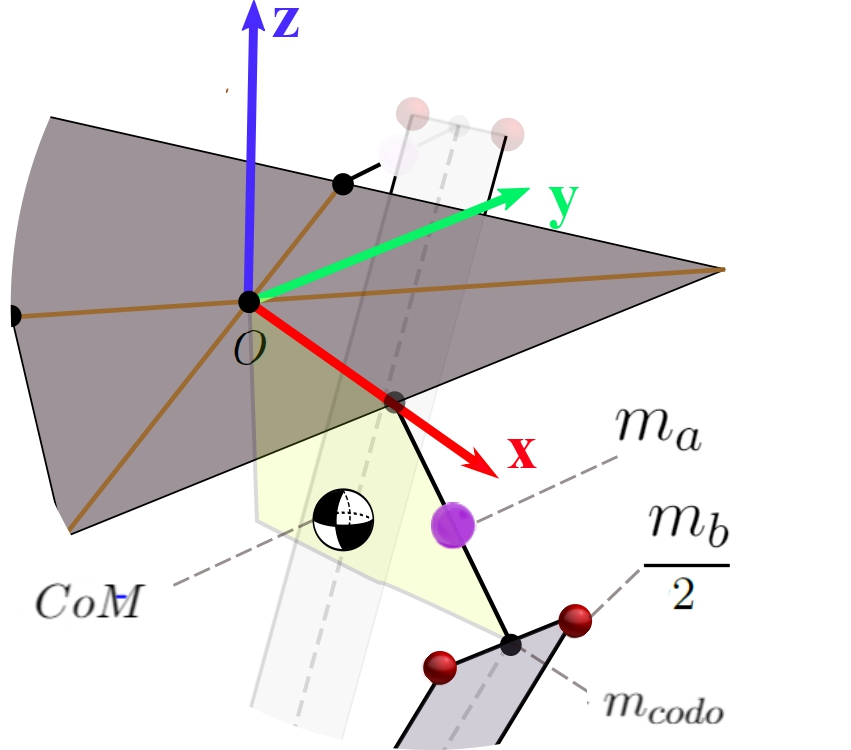
\includegraphics[width=0.7\linewidth]{Main/Chapter4/Images4/DIBUJO41.jpg}
              \caption{Representación gráfica del centro de masas $CoM$}
              \label{f:Cap4_Metodo_B_Modelacion_Dinamica_2}
        \end{figure}
                
                
                
                
                
                El segundo parámetro dinámico importante es la matriz de inercia en el espacio articular, dado en \ref{par_dina_anex_2}:
                \begin{equation}
                 I_{b}= \left[ \begin{matrix}
                I_{b1}  &  0  &  0\\
                0  &  I_{b2}  &  0\\
                0  &  0  &  I_{b3}\\
                \end{matrix}
                 \right]
                \label{par_dina_anex_2}                    
                \end{equation}

                En \ref{par_dina_anex_2},  \( I_{bi} \)  es la inercia de cada brazo que es la suma de la inercia del motor  \( I_{m}\)  y la del brazo, como se expresa a continuación:
                \begin{equation}
                 I_{bi}=I_{m}+ L_{A}^{2} \left( \frac{m_{a}}{3}+m_{codo}+2\ast r\ast m_{b} \right) 
                \end{equation}
                
                Estos parámetros dinámicos se utilizan para derivar el modelo dinámico del robot paralelo delta. 
\newpage

            \subsubsection{Dinámica inversa}
                La parte del efector final consta de la base móvil, la carga útil y las masas concentradas en las extremidades de los antebrazos. La masa de esta porción,  \( m_{nt} \) , se expresa como:
                
                 \[ m_{nt}=m_{c}+m_{payload}+3\ast 2 \ast \left( 1-r \right) m_{b} \] 
                
                donde,  \( m_{payload} \)  es la masa de la carga útil,  \( m_{c} \)  es la masa de la base móvil y  \( m_{b} \)  es la masa de un par de barras paralelas y  \( r \)  es la relación de división de masas del antebrazo.
                
                En el robot paralelo Delta, los únicos dos tipos de fuerzas que actúan sobre el efector final son; la fuerza de gravedad  \( \overrightarrow{F_{g}} \)  y la fuerza de inercia  \( \overrightarrow{F_{in}} \) \  debida a la aceleración:
                
                 \[ \overrightarrow{F_{g}}=m_{nt}~ \left[ 0 0-g \right] ^{T} \] 
                
                 \[ \overrightarrow{F_{in}}=m_{nt}~\overrightarrow{\ddot{P_{0}}} \] 
                
                Debido a la arquitectura del robot delta, la orientación del marco del efector final es siempre paralela al marco de referencia $ \{O$ - $xyz\} $ . Por lo tanto, se ignoran los términos de movimiento rotacional para el efector final.
                
                Como se explicó anteriormente, el principio del trabajo virtual se basa en el supuesto de que la contribución de todas las fuerzas inerciales debe ser igual a la contribución de todas las fuerzas no inerciales. El principio de la ecuación de trabajo virtual para el efector final se puede escribir en su forma vectorial como:
                \begin{equation}
                    \left( \overrightarrow{F_{g}}-m_{nt}~\overrightarrow{\ddot{P_{0}}} \right) \ast \delta r_{E}=0 
                \label{anex_dina_inver_mb_1}
                \end{equation}
                
                donde,  \( g \)  es la aceleración debida a la gravedad,  \( \overrightarrow{\ddot{P_{0}}} \)  es el vector de aceleración del efector final y  \(  \delta r_{E} \) \  es el desplazamiento virtual del efector final.
                
                Para resolver la dinámica del robot, el brazo es formado por un enlace de masa  \( m_{a} \)  y en sus extremidades se agrega las masas puntuales concentradas de las barras paralelas  \(  \left( \frac{m_{b}}{2}+\frac{m_{b}}{2} \right)  \)  . Tres pares actúan sobre los brazos en cualquier momento: el par  \( \overrightarrow{ \tau_{Gb}} \) \  debido a la gravedad que actúa sobre el centro de masa, el par  \( \overrightarrow{ \tau}= \left[  \tau_{1}, \tau_{2}, \tau_{3} \right] ^{T} \)  debido al actuador y el par  \( I_{b}~\overrightarrow{\ddot{ \theta }} \)  debido al momento de inercia  \( I_{b} \)  sobre el eje de rotación. La vector de aceleración angular de los actuadores se representa matricialmente  \( \overrightarrow{\ddot{ \theta }}= \left[ \ddot{ \theta }_{1},\ddot{ \theta }_{2},\ddot{ \theta }_{3} \right] ^{T} \) . La ecuación de trabajo virtual del brazo se expresa de la siguiente manera:
                
                 \[  \left( \overrightarrow{ \tau}-I_{b}~\overrightarrow{\ddot{ \theta }}+\overrightarrow{ \tau_{Gb}} \right) \ast \delta  \theta =0 \] 
                
                Para obtener el para debido a la gravedad, primero se debe calcular el centro de masa  \( CoM \)  del brazo, que incluye las masas puntuales concentradas de las barras paralelas. Una vez determinado el centro se masa, se calcula el torque debido a las fuerzas de gravedad en el brazo con la siguiente expresión:
                \begin{equation}
                 \overrightarrow{ \tau_{Gb}}=g\ast CoM\ast \left( m_{a}+m_{codo}+2\ast r\ast m_{b} \right)  \left[ \cos  \left(  \theta _{1} \right) ~\cos  \left(  \theta _{2} \right) ~\cos  \left(  \theta _{3} \right)  \right] ^{T} 
                \label{anex_dina_inver_mb_2}
                \end{equation}
                                \newpage

                
                Con los parámetros dinámicos para los componentes individuales del manipulador calculados, se puede desarrollar la dinámica completa del robot. Recordando que la suma de todo el trabajo virtual realizado en el sistema por todas las fuerzas y pares externos debe ser igual a cero, se suman las ecuaciones \ref{anex_dina_inver_mb_1} y \ref{anex_dina_inver_mb_2} para determinar el torque en los actuadores  \( \overrightarrow{ \tau} \)  :
                
                 \[  \left( \overrightarrow{F_{g}}-m_{nt}\overrightarrow{\ddot{P_{0}}} \right) \ast \delta r_{E}+  \left( \overrightarrow{ \tau}-I_{b}\overrightarrow{\ddot{ \theta }}+\overrightarrow{ \tau_{Gb}} \right) \ast \delta  \theta =0 \] 
                
                Reemplazando la contribución del desplazamiento  \(  \delta r_{E}=J^{T} \delta  \theta  \) \  en los actuadores:
                
                 \[  \left( \overrightarrow{F_{g}}-m_{nt}\overrightarrow{\ddot{P_{0}}} \right) \ast J \delta  \theta +  \left( \overrightarrow{ \tau}-I_{b}\overrightarrow{\ddot{ \theta }}+\overrightarrow{ \tau_{Gb}} \right) \ast \delta  \theta =0 \] 
                
                Reordenando matricialmente para simplificar la ecuación anterior se llega a que: 
                
                 \[ J^{T}\overrightarrow{F_{g}}-J^{T}m_{nt}\overrightarrow{\ddot{P_{0}}}+\overrightarrow{ \tau}+-I_{b}\overrightarrow{\ddot{ \theta }}+\overrightarrow{ \tau_{Gb}}=0 \] 
                
                 \[ \overrightarrow{ \tau}=I_{b}\overrightarrow{\ddot{ \theta }}+J^{T}m_{nt}\overrightarrow{\ddot{P_{0}}}- J^{T}\overrightarrow{F_{g}}-\overrightarrow{ \tau_{Gb}} \] 
                
                Sustituyendo  \( \overrightarrow{\ddot{P_{0}}}=J\overrightarrow{\ddot{ \theta }}+\dot{J}\overrightarrow{\dot{ \theta }} \) 
                
                 \[ \overrightarrow{ \tau}=I_{b}\overrightarrow{\ddot{ \theta }}+J^{T} m_{nt}  \left( J\overrightarrow{\ddot{ \theta }}+\dot{J} \overrightarrow{\dot{ \theta }} \right) - J^{T}\overrightarrow{F_{g}}-\overrightarrow{ \tau_{Gb}} \] 
                
                 \[ \overrightarrow{ \tau}= \left( I_{b}+J^{T} m_{nt} J \right) \overrightarrow{\ddot{ \theta }}+ \left( J^{T} m_{nt}\dot{J} \right)  \overrightarrow{\dot{ \theta }}+ \left( - J^{T}\overrightarrow{F_{g}}-\overrightarrow{ \tau_{Gb}} \right)  \] 
                
                A partir de (), podemos identificar fácilmente la matriz de masa  \( M \left(  \theta  \right)  \) , la matriz  \( C \left(  \theta ,\dot{ \theta } \right)  \)  de coeficiente de Coriolis y centrífuga, y el vector de términos de gravedad  \( \overrightarrow{G} \left(  \theta  \right)  \)  comparándolo con la dinámica estándar:
                
                 \[ \overrightarrow{ \tau}=M \left(  \theta  \right) \overrightarrow{\ddot{ \theta }}+C \left(  \theta ,\dot{ \theta } \right) \overrightarrow{\dot{ \theta }}+ \overrightarrow{G} \left(  \theta  \right)  \] 
                
                Dónde
                
                 \[ M \left(  \theta  \right) =I_{b}+J^{T} m_{nt} J \] 
                
                 \[ C \left(  \theta ,\dot{ \theta } \right) =J^{T} m_{nt}\dot{J} \] 
                
                 \[ \overrightarrow{G} \left(  \theta  \right) =- J^{T}\overrightarrow{F_{g}}-\overrightarrow{ \tau_{Gb}} \] 
         \newpage

\comment{
This line of text won't show

This one won't either
}
      
...
\end{comment}

%\begin{comment}
\chapter{Carpetas, comandos y códigos}\label{anexoC}
\thispagestyle{fancy}
\pagenumbering{arabic}\renewcommand{\thepage}{B.\arabic{page}}

Se muestra en la figura \ref{f:Cap4_Metodo_B_Modelacion_Dinamica_2} todas las carpetas donde esta la configuración en ROS y RVIZ. Los archivos creados en esta tesis que están contenidos en estas carpetas principalmente: son los algoritmos en lenguaje python de los metodos A, metodo B, espacio de trabajo y trayectorias, los mensajes que se utilizan en los temas de ROS, la configuración URDF del robot delta y la configuracion de la vizualizacion en Rviz. Los archivos se pueden descargar del siguiente repositorio en GitHub: \url{www.bablablabla}.

    \section{Carpetas creadas por catkin make}
        \begin{figure}[H]
              \centering
	          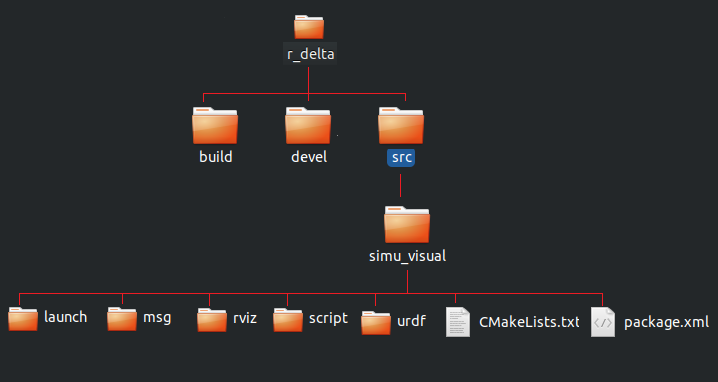
\includegraphics[width=1.0\linewidth]{Back/image_anexo/catkin_make.png}
              \caption{Espacio de trabajo creado por catkin\_make para los algoritmos de los métodos A y B}
              \label{f:Cap4_Metodo_B_Modelacion_Dinamica_2}
        \end{figure}
    \newpage

    \section{Comandos para compilar nodos en shell}
    
    \begin{itemize}
        \item Transformar archivos de nodos a archivos python ejecutables
    \end{itemize}
            \lstset{language=XML}
            \begin{lstlisting}
chmod +x nombre_py_nodo_ejecutable.py
            \end{lstlisting}

    \begin{itemize}
        \item Archivos python que son nodos
    \end{itemize}
            \lstset{language=XML}
            \begin{lstlisting}
Trayectoria y Torques: path_tm1_v2_adams.py
Espacio de trabajo: workspace_v2.py
Visualizacion: posicionador_rviz_realtime_tm1_adams.py
            \end{lstlisting}

    \begin{itemize}
        \item Shell y comandos necesarios para calcular torques de trayectorias
    \end{itemize}
            \lstset{language=XML}
            \begin{lstlisting}
-------- [shell 0]: Para todos los shell 
cd r_delta
source devel/setup.bash

-------- [shell 1]: ROS Master
roscore

-------- [shell 2]: Abrir Rviz
roslaunch simu_visual rviz_tm1_adams.launch

-------- [shell 3]: Nodo visualización
rosrun simu_visual posicionador_rviz_realtime_tm1_adams.py

-------- [shell 4]: Herramienta que grafica nodos iniciados
rosrun rqt_graph rqt_graph

-------- [shell 5]: Nodo de Trayectoria y Torques
rosrun simu_visual path_tm1_v2_adams.py

-------- [shell 6]: Mensaje para el nodo torques y trayectorias (1)
rostopic pub -1 /input_ls_final simu_visual/linear_speed_xyz
"{xo: -300.0, yo: 0.0, zo: -450.0,
xf: 300.0, yf: 150.0, zf: -750.0,
vmax: 2000.0, amax: 40000.0,
paso1: 50,  paso2: 150,
ls_fin: true, idcall: 1, num_tray: 1}"

-------- [shell 6]: Mensaje para el nodo torques y trayectorias (2)
rostopic pub -1 /input_ls_final simu_visual/linear_speed_xyz
"{xo: -300.0, yo: -150.0, zo: -450.0,
xf: 300.0, yf: 150.0, zf: -750.0,
vmax: 2000.0, amax: 40000.0,
paso1: 50,  paso2: 150,
ls_fin: true, idcall: 1, num_tray: 2}"

-------- [shell 6]:  Mensaje para el nodo torques y trayectorias (3)
rostopic pub -1 /input_ls_final simu_visual/linear_speed_xyz
"{xo: 300.0, yo: -150.0, zo: -450.0,
xf: -300.0, yf: 150.0, zf: -750.0,
vmax: 2000.0, amax: 40000.0,
paso1: 50,  paso2: 150,
ls_fin: true, idcall: 1, num_tray: 3}"

-------- [shell 6]: Mensaje para el nodo torques y trayectorias (4)
rostopic pub -1 /input_ls_final simu_visual/linear_speed_xyz
"{xo: 400.0, yo: 150.0, zo: -450.0,
xf: -400.0, yf: 150.0, zf: -450.0,
vmax: 2000.0, amax: 40000.0,
paso1: 50,  paso2: 150,
ls_fin: true, idcall: 1, num_tray: 4}"

-------- [shell 6]: Mensaje para el nodo torques y trayectorias (5)
rostopic pub -1 /input_ls_final simu_visual/linear_speed_xyz
"{xo: -300.0, yo: 0.0, zo: -450.0,
xf: 300.0, yf: 150.0, zf: -750.0,
vmax: 200.0, amax: 10000.0,
paso1: 50,  paso2: 150,
ls_fin: true, idcall: 1, num_tray: 5}"

-------- [shell 6]: Mensaje para el nodo torques y trayectorias (6)
rostopic pub -1 /input_ls_final simu_visual/linear_speed_xyz
"{xo: -300.0, yo: -150.0, zo: -450.0,
xf: 300.0, yf: 150.0, zf: -750.0,
vmax: 200.0, amax: 10000.0,
paso1: 50,  paso2: 150,
ls_fin: true, idcall: 1, num_tray: 6}"

-------- [shell 6]: Mensaje para el nodo torques y trayectorias (7)
rostopic pub -1 /input_ls_final simu_visual/linear_speed_xyz
"{xo: 300.0, yo: -150.0, zo: -450.0,
xf: -300.0, yf: 150.0, zf: -750.0,
vmax: 200.0, amax: 10000.0,
paso1: 50,  paso2: 150,
ls_fin: true, idcall: 1, num_tray: 7}"

-------- [shell 6]: Mensaje para el nodo torques y trayectorias (8)
rostopic pub -1 /input_ls_final simu_visual/linear_speed_xyz
"{xo: 400.0, yo: 150.0, zo: -450.0,
xf: -400.0, yf: 150.0, zf: -450.0,
vmax: 200.0, amax: 10000.0,
paso1: 50,  paso2: 150,
ls_fin: true, idcall: 1, num_tray: 8}"

            \end{lstlisting}


    \begin{itemize}
        \item Espacio de Trabajo
    \end{itemize}
            \lstset{language=XML}
            \begin{lstlisting}
-------- [shell 0]: Para todos los shell 
cd r_delta
source devel/setup.bash
-------- [shell 1]: Nodo  espacio de trabajo
rosrun simu_visual workspace_v2.py
-------- [shell 2]: Mensaje para tema de nodo espacio de trabajo
rostopic pub -1 /input_workspace simu_visual/parameter_ws
"graficar_realtime: true
step: 10
idcall: 1"
            \end{lstlisting}

    
    
    
    
    
    
    \newpage
    
    \section{CMakeLists.txt (/simu\_visual)}
            \lstset{language=XML}

    \begin{lstlisting}
cmake_minimum_required(VERSION 2.8.3)
project(simu_visual)

## Find catkin macros and libraries
## if COMPONENTS list like find_package(catkin REQUIRED COMPONENTS xyz)
## is used, also find other catkin packages
find_package(catkin REQUIRED COMPONENTS
  roscpp
  rospy
  std_msgs
  sensor_msgs
  message_generation
  genmsg
  urdf)

## Generate messages in the 'msg' folder
 add_message_files(
   FILES
   parameter_ws.msg
   linear_speed_xyz.msg
   matriz_path_ls.msg
 )
 
 ## Generate added messages and services with any dependencies listed here
 generate_messages(
   DEPENDENCIES
   std_msgs
 )
 
 catkin_package(
  INCLUDE_DIRS include
  LIBRARIES simu_visual
  CATKIN_DEPENDS roscpp rospy std_msgs message_runtime
  #DEPENDS system_lib
) 
 
include_directories( 
# include 
  ${catkin_INCLUDE_DIRS} 
) 
 
    \end{lstlisting}

    \newpage
    
    \section{Package.xml (/simu\_visual)}
    
        \lstset{language=XML}
        \begin{lstlisting}
<?xml version="1.0"?>
<package format="2">
  <name>simu_visual</name>
  <version>0.0.0</version>
  <description>The simu_visual package</description>

  <!-- One maintainer tag required, multiple allowed, one person per tag -->
  <maintainer email="ivan.fernandez.g@usach.cl">ivan</maintainer>

  <!-- Commonly used license strings: -->
  <license>BSD</license>

  <!-- Use build_depend for packages you need at compile time: -->
  <build_depend>roscpp</build\_depend>
  <build_depend>rospy</build_depend>
  <build_depend>std_msgs</build_depend>
  <build_depend>sensor_msgs</build_depend>
  <build_depend>message_generation</build_depend>

  <!-- Use build_export_depend for packages you need 
  in order to build against this package: -->
  <build_export_depend>roscpp</build_export_depend>
  <build_export_depend>rospy</build_export_depend>
  <build_export_depend>std_msgs</build_export_depend>
  <build_export_depend>message_generation</build_export_depend>

  <!-- Use buildtool_depend for build tool packages: -->
  <buildtool_depend>catkin</buildtool_depend>

  <!-- Use exec_depend for packages you need at runtime: -->
  <exec_depend>roscpp</exec_depend>
  <exec_depend>rospy</exec_depend>
  <exec_depend>std_msgs</exec_depend>
  <exec_depend>sensor_msgs</exec_depend>
  <exec_depend>message_runtime</exec_depend>
  
  <export>
  </export>
</package>

    \end{lstlisting}

    \newpage

    \section{Mensajes (/msg)}
        \subsection{linear\_speed\_xyz.msg}

    \lstset{language=XML}
        \begin{lstlisting}
            float32 xo 
            float32 yo
            float32 zo
            float32 xf
            float32 yf
            float32 zf
            float32 vmax
            float32 amax
            int64 paso1
            int64 paso2
            bool ls_fin
            int64 idcall
            int64 num_tray
        \end{lstlisting}

        \subsection{matriz\_path\_ls.msg}
    \lstset{language=XML}
        \begin{lstlisting}
            bool permiso
            int64 id_call
            float32[] x
            float32[] y
            float32[] z
            float32[] th1
            float32[] th2
            float32[] th3
            float32[] tiempo
        \end{lstlisting}

        \subsection{parameter\_ws.msg}
    \lstset{language=XML}
        \begin{lstlisting}
            bool graficar_realtime
            int64 step
            int64 idcall
        \end{lstlisting}

        \newpage
    \newpage
    
    \section{robot\_urdftm1\_adams.urdf (/urfd)}
    
    \lstset{language=XML}
    \begin{lstlisting}

 <?xml version="1.0"?>

<robot name="Delta_robot">

  <!--BASE SUPERIOR:____________________-->
  <link name="base_link">
    <visual>
      <geometry>
        <cylinder length="0.005" radius="0.210"/>  <!--f/2-->
      </geometry>
      <material name="gris">
        <color rgba="0.55 0.55 0.55 0.5"/>
      </material>
    </visual>
  </link>

  <!--BRAZOS SUPERIORES:____________________-->
  <!--BRAZO_1-->
  <link name="brazo1">
    <visual>
      <origin xyz="0.310 0 0" rpy="0 0 0"/> <!--la = 150-->
      <geometry>
        <box size="0.620 0.003 0.003"/> <!--la = 150-->
      </geometry>
      <material name="blanco">
        <color rgba="0.9 0.9 0.9 1"/>
      </material>
    </visual>
  </link>

  <joint name="base_brazo1" type="revolute">
    <axis xyz="0 1 0"/>
    <limit effort="100.0" lower="0.0" upper="1.8" velocity="0.5"/>
    <parent link="base_link"/>
    <child link="brazo1"/>
    <origin xyz="-0.181865335 0.105 0" rpy="0 0 2.61799"/>
  </joint>

  <!--BRAZO_2-->
  <link name="brazo2">
    <visual>
      <origin xyz="0.310 0 0" rpy="0 0 0"/>
      <geometry>
        <box size="0.620 0.003 0.003"/> <!--la = 150-->
      </geometry>
      <material name="blanco"/>
    </visual>
  </link>

  <joint name="base_brazo2" type="revolute">
    <axis xyz="0 1 0"/>
    <limit effort="100.0" lower="0.0" upper="1.8" velocity="0.5"/>
    <parent link="base_link"/>
    <child link="brazo2"/>
    <origin xyz="0 -0.210 0" rpy="0 0 -1.57075"/>
  </joint>

  <!--BRAZO_3-->
  <link name="brazo3">
    <visual>
      <origin xyz="0.310 0 0" rpy="0 0 0"/>
      <geometry>
        <box size="0.620 0.003 0.003"/> <!--la = 150-->
      </geometry>
      <material name="blanco"/>
    </visual>
  </link>
  <joint name="base_brazo3" type="revolute">
    <axis xyz="0 1 0"/>
    <limit effort="100.0" lower="0.0" upper="1.8" velocity="0.5"/>
    <parent link="base_link"/>
    <child link="brazo3"/>
    <origin xyz="0.181865335 0.105 0" rpy="0 0 0.523599"/>
  </joint>

  <!--BRAZOS INFERIORES:____________________-->

  <!--Ante_BRAZO_1-->
  <link name="barra1_a"/>
  <joint name="codo1_a" type="revolute">
    <axis xyz="0 -1 0"/>
    <limit effort="100.0" lower="-3.14" upper="3.14" velocity="0.5"/>
    <parent link="brazo1"/>
    <child link="barra1_a"/>
    <origin xyz="0.620 0 0" rpy="0 0 0"/>
  </joint>

  <link name="barra1_b">
    <visual>
      <origin xyz="-0.440 0 0" rpy="0 0 0"/> <!--0.175-->
      <geometry>
        <box size="0.880 0.003 0.003"/> <!--lb = 205-->
      </geometry>
      <material name="blanco"/>
    </visual>
  </link>

  <joint name="codo1_b" type="revolute">
    <axis xyz="0 0 1"/>
    <limit effort="100.0" lower="-3.14" upper="3.14" velocity="0.5"/>
    <parent link="barra1_a"/>
    <child link="barra1_b"/>
    <origin xyz="0 0 0" rpy="0 0 0"/>
  </joint>

  <!--Ante_BRAZO_2-->

  <link name="barra2_a"/>
  <joint name="codo2_a" type="revolute">
    <axis xyz="0 -1 0"/>
    <limit effort="100.0" lower="-3.14" upper="3.14" velocity="0.5"/>
    <parent link="brazo2"/>
    <child link="barra2_a"/>
    <origin xyz="0.620 0 0" rpy="0 0 0"/> <!--la = 150-->
  </joint>

  <link name="barra2_b">
    <visual>
      <origin xyz="-0.440 0 0" rpy="0 0 0"/> <!--lb = 205  / 2 -->
      <geometry>
        <box size="0.880 0.003 0.003"/> <!--lb = 205-->
      </geometry>
      <material name="blanco"/>
    </visual>
  </link>

  <joint name="codo2_b" type="revolute">
    <axis xyz="0 0 1"/>
    <limit effort="100.0" lower="-3.14" upper="3.14" velocity="0.5"/>
    <parent link="barra2_a"/>
    <child link="barra2_b"/>
    <origin xyz="0 0 0" rpy="0 0 0"/> <!--O2 = 62.0652 -107.5000 0-->
  </joint>

  <!--Ante_BRAZO_3-->
  <link name="barra3_a"/>
  <joint name="codo3_a" type="revolute">
    <axis xyz="0 -1 0"/>
    <limit effort="100.0" lower="-3.14" upper="3.14" velocity="0.5"/>
    <parent link="brazo3"/>
    <child link="barra3_a"/>
    <origin xyz="0.620 0 0" rpy="0 0 0"/> <!--O2 = 62.0652 -107.5000 0-->
  </joint>

  <link name="barra3_b">
    <visual>
      <origin xyz="-0.440 0 0" rpy="0 0 0"/>
      <geometry>
        <box size="0.880 0.003 0.003"/> <!--lb = 205-->
      </geometry>
      <material name="blanco"/>
    </visual>
  </link>

  <joint name="codo3_b" type="revolute">
    <axis xyz="0 0 1"/>
    <limit effort="100.0" lower="-3.14" upper="3.14" velocity="0.5"/>
    <parent link="barra3_a"/>
    <child link="barra3_b"/>
    <origin xyz="0 0 0" rpy="0 0 0"/> <!--O2 = 62.0652 -107.5000 0-->
  </joint>

  <!--ACTUADOR:____________________-->

  <link name="actuador">
    <visual>
      <origin xyz="0 0 0" rpy="0 -1.57075 0"/>
      <geometry>
        <cylinder length="0.001" radius="0.050"/>
      </geometry>
      <material name="colorte">
        <color rgba="0.15 0.55 0.95 0.3"/>
      </material>
    </visual>
  </link>

  <link name="aux1"/>
  <link name="aux2"/>


  <joint name="act_x" type="prismatic">
    <parent link="base_link"/>
    <child link="aux1"/>
    <limit effort="100.0" lower="-1" upper="1" velocity="0.5"/>
    <origin rpy="0 0 0" xyz="0 0 0"/>
  </joint>

  <joint name="act_y" type="prismatic">
    <parent link="aux1"/>
    <child link="aux2"/>
    <limit effort="100.0" lower="-1" upper="1" velocity="0.5"/>
    <origin rpy="0 0 1.57075" xyz="0 0 0"/>
  </joint>

  <joint name="act_z" type="prismatic">
    <parent link="aux2"/>
    <child link="actuador"/>
    <limit effort="100.0" lower="0" upper="1" velocity="0.5"/>
    <origin rpy="0 -1.57075 0" xyz="0 0 0"/>
  </joint>
</robot>


    \end{lstlisting}

    
    \section{rviz\_tm1\_adams.launch (/launch)}
        \lstset{language=XML}

    \begin{lstlisting}

<launch>
  <!-- comentarios -->
  <arg name="model"/>
  <arg name="gui" default="true"/>
  <param name="robot_description" 
		 textfile="$(find simu_visual)/urdf/robot_urdftm1_adams.urdf"/>
  <param name="use_gui" value="$(arg gui)"/>
  <node name="estados_robot_pub" 
		pkg="robot_state_publisher" type="robot_state_publisher"/>
  <node name="rviz" pkg="rviz" type="rviz" 
		args="−d $(find simu_visual)/rviz/tfm_simulacion.rviz" required="true"/>
</launch>
    \end{lstlisting}

    
    
    \newpage
    
    \section{Python (/script)}
    
%%%%%%%%%%%%%%%% INICIO PRUEBAS &&&&&&&&&&&&&&&&    
    
    % INICIO rodrigo   en desarrolllo
        %\subsection{TEST Códigos Bonitos} 
            %%Python code highlighting

\definecolor{LightGray}{gray}{0.9}
\definecolor{DarkGray}{gray}{0.1}

\usemintedstyle{borland}
% \usemintedstyle{manni}

% \pagecolor{DarkGray}




	

%New colors defined below
% \definecolor{codegreen}{rgb}{0,0.6,0}
% \definecolor{codegray}{rgb}{0.5,0.5,0.5}
% \definecolor{codepurple}{rgb}{0.58,0,0.82}
% \definecolor{backcolour}{rgb}{0.95,0.95,0.92}



% \begin{listing}
\begin{minted}
[
frame=lines,
breaklines=true,
framesep=2mm,
baselinestretch=1.2,
bgcolor=LightGray,
% bgcolor=DarkGray,
fontsize=\footnotesize,
linenos
]
{python}



# Nombre Creador: Ivan Alejandro Fernandez Gracia
# Universidad: Universidad de Santiago de Chile
# Mail: ivan.fernandez.g@usach.cl
# Objetivo: Ingresar parametros para calcular el
# torque de los actuadores de un robot delta

# Importar Librerias
import math


######################################################
##########  Cambio Unidades ##########################
######################################################
def dtr():
 valor = math.pi / 180.0  # Grados a Radianes
 return valor


def rtd():
 valor = 180.0 / math.pi  # Radianes a Grados
 return valor


def mmtm():
 valor = ((10.0) ** (-3))  # Milimetros a Metros
 return valor


def mtmm():
 valor = ((10.0) ** (3))  # Metros a Milimetros
 return valor


def kgm2tgrmm2():
 valor = ((10.0) ** (3 + 6))  # Kilogramo metro^2 a gramo mm^2
 return valor


######################################################
##########  Trigonometria ############################
######################################################
def sqrt3():
 valor = math.sqrt(3.0)
 return valor


def pi():
 valor = math.pi  # [rad]
 return valor


def sin120():
 valor = sqrt3() / 2.0
 return valor


def cos120():
 valor = -0.5
 return valor


def tan60():
 valor = sqrt3()
 return valor


def sin30():
 valor = 0.5
 return valor


def tan30():
 valor = 1.0 / sqrt3()
 return valor


def cos30():
 valor = (sqrt3()) / 2.0
 return valor


######################################################
##########  Dimensionamiento Geometrico Robot Delta ##
######################################################
def l2():
 valor = (880.0) * ((10.0) ** (-3))  # Longitud Antebrazo [m]
 return valor


def l1():
 valor = (620.0) * ((10.0) ** (-3))  # Longitud Brazo [m]
 return valor


def rb():
 valor = (50.0) * ((10.0) ** (-3))  # Radio plataforma movil[m]
 return valor


def ra():
 valor = (210.0) * ((10.0) ** (-3))  # Radio base fija [m]
 return valor


def e():
 valor = (2.0 * rb()) / (tan30())  # [m]
 return valor


def f():
 valor = (2.0 * ra()) / (tan30())  # [m]
 return valor


def hf():
 valor = math.sqrt(0.75 * (f() ** 2))  # [m]
 return valor


def he():
 valor = math.sqrt(0.75 * (e() ** 2))  # [m]
 return valor


######################################################
##########  Masas e Inercias #########################
######################################################
def m1():
 valor = (2213.0) * ((10.0) ** (-3))  # Masa Brazo [kg]
 return valor


def m_elbow():
 valor = (0.0) * ((10.0) ** (-3))  # Masa juntas [kg]
 return valor


def m2():
 valor = (1315.0 / 2.0) * ((10.0) ** (-3))  # Masa de una varilla del antebrazo [kg]
 return valor


def mp():
 valor = (510.0) * ((10.0) ** (-3))  # Masa plataforma movil [kg]
 return valor


def inercia_m():
 valor = (0.0) * ((10.0) ** (-3))  # Inercia actuadores [kg * m2]
 return valor


def gg():
 valor = (9.81)  # Gravedad [m/s2]
 return valor


def r_mass():
 valor = (0.5)  # Relacion de masas del antebrazo
 return valor


def com():
 valor = (l1()) * (((0.5 * (m1())) + (m_elbow()) + ((2) * (r_mass()) * (m2()))) /
				   ((1.0 * (m1())) + (m_elbow()) + ((2) * (r_mass()) * (m2()))))
 # Centro de masas brazo
 return valor


######################################################
##########  Restricciones Espacio de Trabajo #########
######################################################
# Restricciones limines de angulos de motores [grados]
def res_ang_min():
 valor = int(-90)
 # valor=int(-30)
 return valor


def res_ang_max():
 valor = ((res_ang_min()) * -1) + 1
 # valor=90
 return valor


# Restriccion angulos 2 y 3 de cada brazo [grados]
def theta2i_min():
 valor = 5
 return valor


def theta2i_max():
 valor = 180 - theta2i_min()
 return valor


def theta3i_min():
 valor = 45
 return valor


def theta3i_max():
 valor = 180 - theta3i_min()
 return valor


# Restricciones Singularidad Jacobiano
def err_jxx():
 valor = (6) * (10 ** (-1))
 return valor


def err_jinv():
 valor = (4) * (10 ** (-3))
 return valor


# Restriccion del fabricante (caja) [mm]
def px_max_ws():
 valor = 400
 return valor


def px_min_ws():
 valor = (-1) * px_max_ws()
 return valor


def py_max_ws():
 valor = 400
 return valor


def py_min_ws():
 valor = (-1) * py_max_ws()
 return valor


def pz_max_ws():
 valor = -300
 return valor


def pz_min_ws():
 valor = -750
 return valor
 

 \end{minted}
% \caption{Example with line numbers enabled}
% \end{listing}

\clearpage
   % FIN rodrigo  en desarrolllo
            %\newpage    

            
    % INICIO ivan LISTO   OPCION 1
   % \subsection{IVAN LISTO}
   %\begin{code}
    %    {\footnotesize 
    %                \inputminted{python}{Back/codigos_py/pd_tm1_adams.py}
                    %\captionof{listing}{Some caption\label{lst:some-flabel}}
    %                }
    %\end{code}
    
    %\newpage    
      % FIN ivan  en desarrolllo    

  % \begin{code}
   %     {\footnotesize 
    %                \inputminted{python}{Back/codigos_py/.py}}
    %\end{code}
    
    %\newpage       
   
%%%%%%%%%%%%%%%% FIN PRUEBAS &&&&&&&&&&&&&&&&    


        \subsection{pd\_tm1\_adams.py}
        {\footnotesize 
            \inputminted{python}{Back/codigos_py/pd_tm1_adams.py}
            }
        \newpage    
        
        \subsection{path\_tm1\_v2\_adams.py}
        {\footnotesize 
            \inputminted{python}{Back/codigos_py/path_tm1_v2_adams.py}
            }
        \newpage
        
        \subsection{linear\_speed\_f\_adams.py}
        {\footnotesize 
            \inputminted{python}{Back/codigos_py/linear_speed_f_adams.py}
            }
        \newpage
        
        \subsection{trans\_rot\_ls\_adams.py}
        {\footnotesize 
            \inputminted{python}{Back/codigos_py/trans_rot_ls_adams.py}
            }
        \newpage
        
        \subsection{delta\_kinematics\_t1m\_adams.py}
        {\footnotesize 
            \inputminted{python}{Back/codigos_py/delta_kinematics_t1m_adams.py}
            }
        \newpage
        
        \subsection{delta\_kinematics\_Paderborn\_tm1\_adams.py}
        {\footnotesize 
            \inputminted{python}{Back/codigos_py/delta_kinematics_Paderborn_tm1_adams.py}
            }
        \newpage
        

        \subsection{jacobian\_tm1\_adams.py}
        {\footnotesize 
            \inputminted{python}{Back/codigos_py/jacobian_tm1_adams.py}
            }
        \newpage
    
        \subsection{jacobian\_Paderborn\_tm1\_v2\_adams.py}
        {\footnotesize 
            \inputminted{python}{Back/codigos_py/jacobian_Paderborn_tm1_v2_adams.py}
            }
        \newpage    
    
        \subsection{torque\_m1\_adams.py}
        {\footnotesize 
            \inputminted{python}{Back/codigos_py/torque_m1_adams.py}
            }
        \newpage    
        
        \subsection{torque\_m1\_Paderborn\_v2\_adams.py}
        {\footnotesize 
            \inputminted{python}{Back/codigos_py/torque_m1_Paderborn_v2_adams.py}
            }
        \newpage    
        
        \subsection{workspace\_v2.py}
        {\footnotesize 
            \inputminted{python}{Back/codigos_py/workspace_v2.py}
            }
        \newpage   
        
        \subsection{posicionador\_rviz\_realtime\_tm1\_adams.py}
        {\footnotesize 
            \inputminted{python}{Back/codigos_py/posicionador_rviz_realtime_tm1_adams.py}
            }
        \newpage  
        
        \subsection{codos\_tm1\_adams.py}
        {\footnotesize 
            \inputminted{python}{Back/codigos_py/codos_tm1_adams.py}
            }
        \newpage  
%\end{comment}
